\documentclass{StockSense}
\usepackage{multirow}
\usepackage{float}
\usepackage{longtable}
\begin{document}

% ============================================================
% PROJECT INFORMATION
% ============================================================

\newcommand{\supervisor}{Mr. Saifullah Tanvir}
\newcommand{\university}{National University of Computer and Emerging Sciences, Lahore}
\newcommand{\fyptitle}{StockSense}
\newcommand{\degree}{BS}

\newcommand{\Studentone}{Muhammad Usman  23L-0693  BS(CS)}
\newcommand{\Studenttwo}{Muhammad Rizwan Arshad  23L-0755  BS(CS)}
\newcommand{\Studentthree}{Hayyan Haider  23L-0727  BS(CS)}

\date{\today}

\renewcommand{\contentsname}{Table of Contents}


% ============================================================
% TITLE PAGE
% ============================================================

\makeatletter

\begin{titlepage}

    
\includegraphics[width=0.2\linewidth]{Figures/nulogo.png}
    \hfill
    
\includegraphics[width=0.2\linewidth]{Figures/fast.png}\\

    \begin{center}

        {\large\bfseries \university}\\[7ex]

        
\includegraphics[width=0.4\linewidth]{Figures/fastlogo.png}\\[8ex]

        {\huge \bfseries \fyptitle}\\[10ex]

        {\Studentone}\\
        {\Studenttwo}\\
        {\Studentthree}\\[4ex]

        {Supervisor: \supervisor}\\[10ex]

        {Final Year Project}\\

        {\large \@date}

    \end{center}

\end{titlepage}

\makeatother


% ============================================================
% FRONT MATTER
% ============================================================

\frontmatter
\pagestyle{fancy}

\newpage
\thispagestyle{empty}
\mbox{}
\newpage


% ============================================================
% ANTI-PLAGIARISM DECLARATION
% ============================================================

\section*{\begin{center}
Anti-Plagiarism Declaration
\end{center}}

This is to declare that the above publication was produced under the:

\begin{flushleft}
\bf Title: \fyptitle
\end{flushleft}

is the sole contribution of the author(s), and no part hereof has been reproduced as it is the basis (cut and paste) that can be considered Plagiarism. All referenced parts have been used to argue the idea and cited properly. I/We will be responsible and liable for any consequence if a violation of this declaration is determined.

\vspace{4ex}

Date: ..........................

\begin{flushright}

Name: Muhammad Usman

\vspace{3ex}

Signature: \quad\begin{tabular}[b]{@{}c@{}}

\includegraphics[width=4.5cm,height=1.2cm]{Figures/usman_sign.png}\\[-5.0ex]
\makebox[5cm]{\dotfill}
\end{tabular}

\vspace{6ex}

Name: Muhammad Rizwan Arshad

\vspace{3ex}

Signature: \quad\begin{tabular}[b]{@{}c@{}}

\includegraphics[width=4.5cm,height=1.2cm]{Figures/rizwan_sign.png}\\[-5.0ex]
\makebox[5cm]{\dotfill}
\end{tabular}

\vspace{6ex}

Name: Hayyan Haider

\vspace{3ex}

Signature: \quad\begin{tabular}[b]{@{}c@{}}

\includegraphics[width=4.5cm,height=1.2cm]{Figures/hayyan_sign.png}\\[-5.0ex]
\makebox[5cm]{\dotfill}
\end{tabular}

\end{flushright}


% ============================================================
% AUTHOR'S DECLARATION
% ============================================================

\vspace{5cm}

\hrule

\section*{Author's Declaration}

This states Authors’ declaration that the work presented in the report is their own, and has not been submitted/presented previously to any other institution or organization.

\pagebreak


% ============================================================
% ABSTRACT
% ============================================================

\section*{Abstract}

Retailers lose money daily when a product, like clothing, footwear or any other physical product with variants, sizes or stores, is out of stock or dead stock. For large chains, the solution is enterprise forecasting systems such as SAP and Blue Yonder, which small businesses can't afford to purchase or maintain. This project aims to develop a multi-tenant SaaS application using a general purpose forecasting engine which can be applicable to any stock-keeping business, called StockSense. It features a free point of sale (POS) solution, location- and variant-level demand forecasting, a markdown/discount optimizer and stock-redistribution suggestions are available as paid subscription options. However, StockSense differs from current tools in that it recommends inter-branch redistribution as its top priority, and alerts the officer with an alert early enough that they can act on it before it becomes a "dead stock", not after it has already died. Existing businesses using a POS or spreadsheets can sign up with uploading their sales reports.

\pagebreak


% ============================================================
% EXECUTIVE SUMMARY
% ============================================================

\section*{Executive Summary}

Retailers face two opposing problems each day that cost them revenue. Dead stock is stored for months, requiring capital and space, while stock outs result in loss of sales as the item the customer is interested in is not available, and less popular items are increasing in quantity. This affects any retailer that manages physical inventory across variants, sizes, or store locations, from clothing and footwear shops to many other kinds of stores. The issue is most severely felt in smaller businesses because restocking decisions are typically made based on instinct. No systematic understanding of what items at what locations meet demand; a manager reorders what he or she thinks sold well.

Large retailers solve this problem by using enterprise demand-forecasting platforms like SAP and Blue Yonder, but these are also expensive and designed for those with an established data team and ERP system. Larger retailers may be able to add another forecasting service to the top of their ERP. Small retailers using basic POS systems or spreadsheets lack an equivalent solution. Even the lighter of inventory software solutions for small businesses usually provide aggregate forecasts (demand predicted per product, not per size or variant), reorder points (alerts only when stock runs low), and slow-mover reports (lists items that already sold poorly), and work with each store's inventory as a separate entity.

To fill this gap, StockSense is a multi-tenant SaaS platform. It is based on a general purpose forecasting engine which can be used for any business where stocks are kept, not just a particular product category. The platform enables small retailers to get a free POS that allows them to record sales and keep an eye on stock and brings their data to the platform, meeting a day-to-day requirement. In addition to that data, a paid subscription opens up the location and variant level demand forecasts and provides an automated markdown/discount optimizer and stock-redistribution recommendations. Companies that already use another point-of-sale system or spreadsheets can join without having to change anything, simply by uploading their previous sales data in CSV or Excel format. In both, owners and managers access their past sales data, current prediction and suggestions for restocking via a simple web dashboard accessible to non-technical users.

StockSense differs from existing solutions in three main ways. First, it prioritizes redistribution. Existing tools generate recommendations for each store independently and mention stock transfers only as one tactic among several. If a business has 2, 3 or more branches, it is almost always cheaper and faster to move unsold stock from a branch where it is not selling to a branch where it is sold, than to sell the same stock at a discount or place a new order – StockSense identifies this as a first class recommendation, ahead of markdowns or reordering.

Second, its intervention is preventive rather than reactive. Existing technologies see stock as dead when it is too old to be a viable option, and then offer write-off or discount. The stock problem now becomes a timing problem because StockSense markdown optimizer detects a stock as it is coming to a slowdown and alerts the manager in time to take action. Thirdly, all recommendations are explained. Every suggestion is accompanied by a simple explanation of why it is warranted and an estimate of the cost, so that a business owner can better understand and be confident in the suggestion rather than blindly following it as a black box.

Preliminary work has included a review of the demand-forecasting and small-business inventory literature, surveying the available enterprise and small-business platforms, and identifying available public retail sales datasets for initial model development and validation. We could not find any platform that offers a free POS system with a possibly paid dead-stock-reduction layer to help small retailers, making StockSense dead-stock-reduction layer freemium seem to be the only one of its kind. The accuracy of the forecast will be judged using standard error metric and potential reduction of dead stock will be simulated with historical data.

To summarize, StockSense was designed to help a small business leverage the sales data that they already gather, but never analyze, to make actionable and inexpensive decisions to decrease dead stock and recover lost sales. It makes demand forecasting and inventory optimization, something traditionally only large retailers have access to, available to small businesses.

\pagebreak


% ============================================================
% TABLE OF CONTENTS
% ============================================================

\pagestyle{fancy}

\tableofcontents

\pagebreak

\addcontentsline{toc}{chapter}{List of Figures}
\listoffigures

\pagebreak

\addcontentsline{toc}{chapter}{List of Tables}
\listoftables

\mainmatter

% ============================================================
% CHAPTER 1
% ============================================================

\chapter{Introduction}

Retailers need the right products in the right quantities and locations, but small and medium-sized businesses often rely on spreadsheets, basic POS systems, or manual records without systematically analyzing sales data. This can cause stock outs and dead stock, particularly when demand for different products, sizes and locations is different in different branches. Large retailers have enterprise forecasting and inventory optimization tools, but these are expensive and difficult to use. StockSense is proposed as a multi-tenant SaaS solution that makes data-driven inventory management more accessible through a free POS system, demand forecasting, inter-branch stock redistribution, markdown optimization, and explainable recommendations. StockSense leverages existing sales data to enable retailers to detect inventory risks early and take action before products become unsold stock or cause stock outs.



\section{Purpose of this Document}

This document provides a detailed description of the StockSense Final Year Project (FYP), which aims to develop a multi-tenant SaaS platform for retail inventory management and demand forecasting. It provides small and medium-sized retailers with an easy-to-use solution to transform POS and historical sales data into actionable inventory decisions. The document covers the project’s problem domain, objectives, scope, requirements, methodology, system design, and implementation, including demand forecasting, inventory redistribution, markdown recommendations, and explainable decision support.


\section{Intended Audience}

The main target audience for this report are the Final Year Project evaluation panel, the project supervisor, software developers, researchers, and stakeholders who are interested in retail inventory management and demand forecasting. It has also been written with the reader in mind who would like to learn about the use of data-driven technologies for small and medium sized retailers in order to better plan their inventories and minimize risk from excess inventory and stock out situations.

\section{Definitions, Acronyms, and Abbreviations}

\textbf{StockSense}: The proposed multi-tenant SaaS platform for retail inventory management, demand forecasting, and inventory recommendations.

\textbf{FYP}: Final Year Project.

\textbf{POS}: Point of Sale.

\textbf{SaaS}: Software as a Service.

\textbf{AI}: Artificial Intelligence.

\textbf{ML}: Machine Learning.

\textbf{ERP}: Enterprise Resource Planning.

\textbf{CSV}: Comma-Separated Values.

\textbf{UI}: User Interface.

\textbf{UX}: User Experience.

\textbf{API}: Application Programming Interface.

\textbf{CRUD}: Create, Read, Update, Delete.

\textbf{MVP}: Minimum Viable Product.

\textbf{SMR}: Small and Medium-sized Retailers.

\section{Conclusion}

In conclusion, StockSense is recommended to support small and medium business-store owners in better decision making on inventory management, by combining sales management and actionable sales recommendations and forecasting. The platform is centered around the challenge of stock out and dead stock - stock out at the product level, dead stock at the variant and location level. It also features prioritizing the movement of current stock between branches when necessary and also identifies slow moving stock quickly enough to take preventative measures.

This project merges a free POS layer with subscription-based forecasting and inventory optimization capabilities for businesses to leverage their existing sales data without the need of a complex enterprise system. StockSense aims to bring inventory analytics to smaller retailers by forecasting, redistribution recommendations, markdown optimization, and easy-to-understand explanations of recommendations. The vision and requirements of the project is presented in detail in the following chapters, along with related work, methodology and system design.

% ============================================================
% CHAPTER 2
% ============================================================

\chapter{Project Vision}

StockSense aims to give the small and medium sized retailer a low cost solution for analyzing their sales pattern and making data-driven decisions on stock. It targets any retailer that stocks physical products with variants, sizes, or multiple stores, such as clothing, footwear, and similar goods, where demand fluctuates greatly by product, size and store location.

\section{Problem Domain Overview}

Retail inventory management is a process that’s used to decide what products should be offered, how much, and where. For small businesses these are normally made based on experience and intuition more than formal forecasting. However, StockSense solves this issue by gathering historical sales data and then applying it to forecast demand across product size and location, and then making a recommendation – for instance, reordering stock, moving stock from one branch to another, or even discounting stock that is on the verge of expiring. The system is supposed to be multi tenant software-as-a-service (SaaS) with each business being a standalone tenant that maintains its own products, stores, inventory, sales, forecasts and recommendations. Historical sales reports can be uploaded as a csv or excel file for businesses with an external POS or spreadsheet, or sales can be recorded by businesses with the built-in POS functionality.

\section{Problem Statement}

There is no affordable, easy-to-use solution that can analyze past sales and make product, size and location product recommendations that can be turned into stock changes. If there were no such system, retailers would have to judge manually, leading to overstocking, dead stock, over-investment in products that don't sell and loss of sales due to stockouts of popular items or sizes.

\section{Problem Elaboration}

The main problems addressed by StockSense are:

\begin{itemize}
    \item Retailers lack the tools to analyze there previous sales data.
    \item Existing enterprise demand-forecasting solutions can be expensive and technically complex for small businesses.
    \item Demand can differ between stores, making aggregate product-level forecasts insufficient.
    \item Demand can also differ significantly between product sizes or variants.
    \item A store may have excess inventory while another branch needs the same product.
    \item Slow-moving inventory may only be identified after it has already become dead stock.
    \item Business owners could find machine-learning-based recommendations difficult to trust if the reasoning behind them is not explained.
\end{itemize}

\section{Goals and Objectives}

The main objectives of StockSense are:

\begin{itemize}
    \item Design a multi-tenant platform that allows multiple small businesses to securely manage their sales and inventory data.
    \item Develop a data ingestion and cleaning pipeline for CSV and Excel sales reports, normalized into a schema of product, size, store/location, date, and quantity sold.
    \item Develop a demand-forecasting model for product-size-location combinations.
    \item Develop a recommendation engine that determines what to reorder, how much to reorder, and where existing inventory should be redistributed.
    \item Develop a markdown/discount optimizer for slow-moving stock.
    \item Provide explanations and estimated financial impact for every recommendation.
    \item Evaluate forecast performance using standard forecasting error metrics and estimate potential dead-stock reduction through historical-data simulation.
    \item Provide the platform under a freemium model consisting of a free POS layer and paid forecasting and recommendation features.
\end{itemize}

\section{Project Scope}

StockSense target companies have products like clothing, footwear, or any other physical product with variants, sizes, or stores that are out of stock or dead stock. It will allow several companies to be tenants on the platform with their stores, products, inventories and sales history being managed separately. The system will enable multi-tenant business management, store and product/variant management, sales and inventory recording over POS, CSV/Excel historical data upload, data cleaning/normalization, product-size-location demand forecast, inventory redistribution/reordering recommendations, markdown and discount recommendations, explainable recommendations with estimated impact on finances, visualization in dashboard.

First, the forecasting period will be targeted on weekly and monthly demand, instead of a long-term prediction of the trend. For full automatic POS integrations to external systems, it's probably a stretch, but manual/batch upload (CSV/Excel) will be supported with the core data-ingestion mechanism.

\section{Sustainable Development Goal (SDG)}

StockSense aligns with the following United Nations Sustainable Development Goals.

\subsection{SDG-8 (Decent Work and Economic Growth)}

The technology that StockSense provides and enables is something that previously was a privilege of the large retailer and StockSense is unlocking and enabling for small retailers, helping to grow and improve the productivity of small enterprises, which are a primary driver of jobs.

\subsection{SDG-9 (Industry, Innovation, and Infrastructure)}

By providing data-driven innovation, StockSense helps retailers more effectively utilize existing capital, stores space and stock, and minimize excess accumulation of unsold inventory, helping to use resources responsibly.

\section{Constraints}

The main challenges of StockSense are: lack and quality of historical sales data, a new business must first enter or upload some sales history before its model can be trained and forecasts become available, forecast accuracy depends on data quality and quantity, public datasets are not necessarily representative of the actual behavior of small retailers, and the focus on products like clothing, footwear or any other physical product and an initial focus on short to medium term demand

\section{Business Opportunity}

StockSense is a freemium SaaS startup. The basic POS features are included for free, enabling small businesses to keep track of their inventory and sales without paying any subscription fees. A paid subscription provides advanced functionality, such as demand forecasting, inventory redistribution, markdown optimization, benchmarking, and explainable financial recommendations. This model enables companies to start leveraging the platform with a minimum upfront investment, yet offers the potential for a seamless evolution for stores aiming advanced analytics.

\section{Stakeholders Description / User Characteristics}

The key users of StockSense are business owners, who view business level performance, inventory, forecasts, and recommendations; branch managers, who view inventory level performance, sales, forecasts, and recommendations for their branch; and the system administrator, who manages overall platform level operations, tenants, subscriptions, and system configuration.

\begin{table}[H]
\centering
\caption{Stakeholders of StockSense}
\begin{tabular}{|l|p{9cm}|}
\hline
\textbf{Stakeholder} & \textbf{Responsibilities} \\ \hline
Business Owner & Monitor business performance, inventory, forecasts, and recommendations. \\ \hline
Store Manager & Monitor branch-level sales, inventory, forecasts, and stock movement. \\ \hline
System Administrator & Manage tenants, platform configuration, and system-level operations. \\ \hline
\end{tabular}
\end{table}

\subsection{Key High-Level Goals and Problems of Stakeholders}

Business owners need an easy solution that makes existing sales data into meaningful inventory decisions. Managers need to see what they're selling and the demand for it at the store level. The system administrator needs ways to keep tenants separate and platform running. The common problem is that there's no simple, affordable system which can integrate sales recording, forecasting and inventory suggestions into a single platform.

\section{Conclusion}

This chapter explained the problem domain, goals, scope, and the stakeholders of StockSense. This platform focuses on providing a solution that helps small and medium-sized businesses leverage existing sales data to inform actionable business decisions for inventory management—without the expense or complexity of enterprise solutions. The next chapter examines the literature and current commercial products related to this project.

% ============================================================
% CHAPTER 3
% ============================================================

\chapter{Literature Review / Related Work}

This chapter summarizes the academic research on problem formulation, demand forecasting, inventory redistribution and markdown optimization, as well as reviews commercial platforms that are relevant to similar problems. This chapter ends with an identification of the gap StockSense is intended to fill and the modeling approach that was chosen for this project.

\section{Definitions and Acronyms}

\subsection{Definitions}

\textbf{Demand forecasting}: The process of estimating future customer demand for a product using historical sales data. \\
\textbf{Lateral transshipment}: The movement of inventory between locations at the same level of a supply chain, such as between two retail branches, rather than from a warehouse. \\
\textbf{Markdown optimization}: The process of determining the size and timing of a price discount to sell slow-moving inventory before it becomes unsellable. \\
\textbf{SKU}: Stock Keeping Unit, a unique identifier for a specific product variant (e.g., a particular size and colour).

\subsection{Acronyms}

\textbf{MAPE}: Mean Absolute Percentage Error. \\
\textbf{RMSE}: Root Mean Squared Error. \\
\textbf{ERP}: Enterprise Resource Planning. \\
\textbf{POS}: Point of Sale. \\
\textbf{ML}: Machine Learning.

\section{Detailed Literature Review}

\subsection{Exploring the Use of Deep Neural Networks for Sales Forecasting in Fashion Retail (Loureiro et al., 2018)}

\textbf{Summary:} Loureiro, Migu\'eis, and da Silva~\cite{loureiro2018deep} compare deep neural networks against shallow methods such as support vector regression for forecasting the sales of new fashion products, using a real dataset from a fashion retailer. They combine data-mining features describing a product's physical and distribution characteristics with expert-defined predictive variables.

\textbf{Critical Analysis:} The study not only shows the superiority of deep learning over shallow models for new-product sales forecasting in the fashion retail domain, but it also uses a real company dataset and not a synthetic one. It does make a prediction at the new product level, though, and the data is from a single large retailer; this doesn't make the results of this model easy to apply to a small enterprise with numerous outlets.

\textbf{Relationship to StockSense:} This paper justifies the selection of learning-based demand forecasting over demand estimation done manually and the use of product attributes as predictive features is directly connected to how StockSense will have to forecast demand for a product in a specific store.

\subsection{Clearance Pricing Optimization for a Fast-Fashion Retailer (Caro and Gallien, 2012)}

\textbf{Summary:} Caro and Gallien~\cite{caro2012clearance} describe a forecasting-and-optimization process that replaced Zara's manual markdown decision-making. A field experiment across all Belgian and Irish stores during a fall-winter season showed the new process increased clearance revenue by approximately six percent, and the process was subsequently adopted company-wide.

\textbf{Critical Analysis:} It's an uncommon, documented and now applied – at scale, with a revenue impact – markdown-optimization model. The major drawback of it for StockSense is that it is intended for a very large vertically-integrated retailer, with extensive historical pricing data for thousands of styles, that will not exist in many of the small retailers at which StockSense operates.

\textbf{Relationship to StockSense:} The paper confirms the fundamental concept behind StockSense' markdown optimizer: A formal forecasting/pricing process can be better than a manual and instinctual markdown decision. StockSense takes this concept and applies it to a smaller data set, but with a mindset of “markdown” not as a clearance-event process for large retailers, but as a “preventive, early-warning” measure.

\subsection{Inventory Models with Lateral Transshipments: A Review (Paterson et al., 2011)}

\textbf{Summary:} Paterson, Kiesm\"uller, Teunter, and Glazebrook~\cite{paterson2011inventory} review the academic literature on lateral transshipments — stock movements between locations of the same echelon — categorizing research by whether transshipments are proactive (planned in advance) or reactive (triggered by a stockout).

\textbf{Critical Analysis:} As a review paper, it provides broad coverage of transshipment models and clearly identifies gaps in the literature, but it does not propose a specific algorithm suited to a small retailer with only two or three branches, nor does it address how transshipment decisions should be combined with markdown or reorder decisions.

\textbf{Relationship to StockSense:} This review establishes the academic basis for treating inter-branch stock transfer as a distinct decision from reordering or discounting. StockSense builds on the proactive-transshipment framing described here, since its redistribution recommendations are intended to prevent dead stock and stockouts before they occur, rather than reacting to an empty shelf.

\subsection{Forecasting Across Time Series Databases Using Recurrent Neural Networks on Groups of Similar Series: A Clustering Approach (Bandara et al., 2020)}

\textbf{Summary:} Bandara, Bergmeir, and Smyl~\cite{bandara2020forecasting} propose clustering related time series and training a single global recurrent neural network per cluster, rather than one model per series, to improve forecast accuracy when individual series have limited history.

\textbf{Critical Analysis:} The clustering-based global model approach is well suited to situations with many short or sparse series, which is a strong match for a small retailer's sales history. A limitation is that the approach was evaluated primarily on general time-series benchmarks rather than retail-specific size- and store-level sales data.

\textbf{Relationship to StockSense:} This paper supports StockSense's choice of a single shared forecasting model trained across many products and stores, rather than one model per product-size-store combination, since an individual small retailer's sales series are often too short for an accurate standalone model.

\subsection{M5 Accuracy Competition: Results, Findings, and Conclusions (Makridakis et al., 2022)}

\textbf{Summary:} Makridakis, Spiliotis, and Assimakopoulos~\cite{makridakis2022m5} report the results of the M5 forecasting competition, in which thousands of teams forecasted 42,840 hierarchical retail sales series for Walmart. The competition found that machine-learning approaches, particularly gradient-boosted tree models such as LightGBM, consistently outperformed traditional statistical methods.

\textbf{Critical Analysis:} The M5 competition is one of the most rigorous, large-scale empirical comparisons of forecasting methods in retail, and its findings are widely cited as a benchmark for which model families perform well on real retail sales data. Its scale, however, reflects a very large retailer with extensive historical data; the competition does not directly address forecasting for small retailers with short sales histories.

\textbf{Relationship to StockSense:} The competition's conclusion that gradient-boosted trees outperform simpler statistical baselines on hierarchical retail sales data directly informs the selection of a forecasting model family for StockSense's product-size-location forecasts.

\subsection{Demand Forecasting for Improved Inventory Management in Small and Medium-Sized Businesses (Purnamasari et al., 2023)}

\textbf{Summary:} Purnamasari, Permadi, Saepudin, and Agusdin~\cite{purnamasari2023demand} compare machine-learning approaches, including an ensemble gradient-boosting model, against classic statistical projection methods for demand forecasting in small leathercraft businesses, using K-means clustering to group products by similarity before forecasting.

\textbf{Critical Analysis:} This is one of the few studies that directly targets small-business demand forecasting rather than large retail chains, and its finding that machine-learning methods outperform classic statistical approaches is directly relevant. The study is limited to a single small-business dataset in one product category, and does not address size- or location-level demand.

\textbf{Relationship to StockSense:} This paper is the most similar to StockSense in terms of its target audience – a small business with no data-science team. Its finding that gradient-boosting-based methods outperform classic statistical approaches on small-business sales data supports StockSense's choice of a gradient-boosted model with statistical baselines for comparison.

\subsection{Retail Forecasting: Research and Practice (Fildes et al., 2022)}

\textbf{Summary:} Fildes, Ma, and Kolassa~\cite{fildes2022retail} present a comprehensive review of academic research in retail forecasting encompassing strategic, tactical and operational forecasting requirements and explore the disconnect between academic forecasting research and practice in retail stores.

\textbf{Critical Analysis:} It is a survey of the field, and thus can serve as a map of the retail-forecasting research landscape, and clearly shows that new-product forecasting is not studied as much as product forecasting. It is a review and does not itself propose or test a model.

\textbf{Relationship to StockSense:} The paper's finding that most published research and tools focused on retail forecasting still rely on a data-science team and an IT infrastructure is consistent with the premise of this project: that existing research and tools are not well suited to small retailers, and StockSense aims to address this gap.

\subsection{Principles and Algorithms for Forecasting Groups of Time Series: Locality and Globality (Montero-Manso and Hyndman, 2021)}

\textbf{Summary:} Montero-Manso and Hyndman~\cite{montero2021principles} describe conditions under which it is preferable to predict a set of related time series using a shared (global) model rather than a separate (local) model for each series, and demonstrate that global models can outperform local models even when there is no obvious similarity between the series.

\textbf{Critical Analysis:} The paper offers a sound theoretical and empirical foundation for global forecasting models, directly applicable to justify StockSense's model-selection approach. It is a general time-series paper, not a retail-specific one, so its recommendations need to be adapted to the specific structure of product-size-store sales data.

\textbf{Relationship to StockSense:} This theoretical result supports StockSense's use of one shared forecasting model across all of a tenant's products and stores, rather than training a separate model for each product-size-store series, since the latter would require more historical data than a small retailer is likely to have.

\subsection{Reducing the Cost of Demand Uncertainty Through Accurate Response to Early Sales (Fisher and Raman, 1996)}

\textbf{Summary:} Fisher and Raman~\cite{fisher1996reducing} show that fashion retailers who shorten lead times and react to early-season sales, rather than committing to production and ordering decisions months in advance, can substantially cut costs. Applied with a major ski-wear firm, their method increased profits by roughly 60\% relative to the firm's existing informal response process.

\textbf{Critical Analysis:} This is a classic, field-validated result demonstrating that acting on early demand signals outperforms manual, instinct-based stocking decisions. Its limitation for StockSense is that it addresses a single-season production and ordering decision for one retailer, rather than ongoing, store-level redistribution between branches.

\textbf{Relationship to StockSense:} This paper is early, influential evidence for the general principle StockSense is built on: that reacting quickly to observed demand, rather than waiting for stock to sit unsold, reduces both lost sales and excess inventory. It supports treating recent sales velocity as a key signal for both the recommendation engine and the markdown optimizer.

\subsection{Sales Forecasts in Clothing Industry: The Key Success Factor of the Supply Chain Management (Thomassey, 2010)}

\textbf{Summary:} Thomassey~\cite{thomassey2010sales} reviews forecasting practices in the clothing industry and proposes forecasting models designed to handle the short life cycles, strong seasonality, and sparse historical data typical of apparel sales.

\textbf{Critical Analysis:} The paper directly addresses the data sparsity and seasonality problems that make apparel demand forecasting harder than forecasting for staple goods, which is highly relevant to StockSense's target product categories. It is focused on a single national clothing distributor, so its specific models may not transfer directly to a small multi-branch retailer.

\textbf{Relationship to StockSense:} This paper reinforces the project's recognition that size- and variant-level apparel demand is noisier and more seasonal than product-level demand overall, supporting StockSense's decision to forecast at the product-size-location level rather than at the product level alone.

\subsection{Predictive Big Data Analytics for Supply Chain Demand Forecasting: Methods, Applications, and Research Opportunities (Seyedan and Mafakheri, 2020)}

\textbf{Summary:} Seyedan and Mafakheri~\cite{seyedan2020predictive} survey the methods and applications of big-data-driven demand forecasting across supply chains, classifying approaches and identifying open research gaps.

\textbf{Critical Analysis:} As a broad survey, it usefully maps the landscape of data-driven forecasting techniques and highlights that most existing applications assume large, centrally managed supply chains with dedicated analytics capability. It does not propose or test a specific model itself.

\textbf{Relationship to StockSense:} This survey's identification of a gap between advanced forecasting techniques and organizations lacking analytics infrastructure reinforces the premise of this project: that small retailers are left out of advances that assume a data team is already in place.

\subsection{Forecasting: Theory and Practice (Petropoulos et al., 2022)}

\textbf{Summary:} Petropoulos et al.~\cite{petropoulos2022forecasting} provide a wide-ranging review of forecasting theory, methods, and practice, covering model selection, evaluation, and the practical challenges of deploying forecasts in real organizations.

\textbf{Critical Analysis:} The review's breadth makes it a useful reference point for forecast evaluation practices and model-selection principles, though, being an encyclopedic review, it does not focus specifically on retail or small-business contexts.

\textbf{Relationship to StockSense:} The paper's guidance on forecast evaluation and model selection informs how StockSense will compare its gradient-boosted forecasting model against simpler statistical baselines, as described in the forecast evaluation approach adopted for this project.

\subsection{From Predictive to Prescriptive Analytics (Bertsimas and Kallus, 2020)}

\textbf{Summary:} Bertsimas and Kallus~\cite{bertsimas2020predictive} propose a framework for converting predictive models into prescriptive decisions, demonstrating their approach on a real inventory-management problem for a large media distributor.

\textbf{Critical Analysis:} The paper is a strong theoretical basis for moving beyond a plain forecast to an actionable decision, which is central to how StockSense is meant to work. Its demonstrated case involves a very large-scale distribution operation, which is a different setting from a small multi-branch retailer.

\textbf{Relationship to StockSense:} This paper supports StockSense's core design choice of not stopping at a forecast, but converting it directly into a concrete, actionable recommendation (redistribution, reorder, or markdown), which is the basis of the recommendation engine described in this project.

\subsection{Stop Explaining Black Box Machine Learning Models for High Stakes Decisions and Use Interpretable Models Instead (Rudin, 2019)}

\textbf{Summary:} Rudin~\cite{rudin2019stop} argues that for high-stakes decisions, inherently interpretable models should be used instead of black-box models paired with separate explanation techniques, since post-hoc explanations of black-box models can be unreliable.

\textbf{Critical Analysis:} The argument is well-supported and widely cited, though it is framed around high-stakes domains such as criminal justice and healthcare rather than retail inventory decisions, where the stakes of an individual recommendation are comparatively low.

\textbf{Relationship to StockSense:} While StockSense's recommendations are lower-stakes than the domains Rudin discusses, the same underlying concern applies: a business owner is unlikely to trust or act on a recommendation they cannot understand. This supports StockSense's design choice to generate a plain-language explanation alongside every recommendation, rather than presenting an unexplained output.

\subsection{Desperately Seeking Shelf Availability: An Examination of the Extent, the Causes, and the Efforts to Address Retail Out-of-Stocks (Corsten and Gruen, 2003)}

\textbf{Summary:} Corsten and Gruen~\cite{corsten2003desperately} report on a worldwide study of retail out-of-stocks, finding that stockout rates had not improved over the preceding decade despite industry efforts, and that a meaningful share of customers switch stores entirely rather than switch products when faced with an out-of-stock.

\textbf{Critical Analysis:} This is a large-scale, widely cited study that establishes stockouts as a persistent, costly, and customer-facing problem, grounding the motivation for this project in real consumer behavior rather than only internal cost. The study focuses on fast-moving consumer goods, not apparel or footwear specifically.

\textbf{Relationship to StockSense:} This paper strengthens the business case for prioritizing redistribution and timely reordering: since customers facing a stockout may leave the store entirely rather than buy a different item, preventing a stockout has a larger business impact than simple lost-sale accounting would suggest.

\section{Literature Review Summary Table}

\scriptsize
\setlength{\LTleft}{0pt}
\setlength{\LTright}{0pt}
\captionof{table}{Summary of Literature Review}\label{tab:literature-review}
\begin{longtable}{@{}|p{0.35cm}|p{2.3cm}|p{0.7cm}|p{4.9cm}|p{4.9cm}|@{}}
\hline
\textbf{No.} & \textbf{Paper Title} & \textbf{Year} & \textbf{Summary} & \textbf{Relevance to StockSense} \\ \hline
\endfirsthead
\textbf{No.} & \textbf{Paper Title} & \textbf{Year} & \textbf{Summary} & \textbf{Relevance to StockSense} \\ \hline
\endhead
\hline
\multicolumn{5}{r}{Continued on next page} \\
\endfoot
\hline
\endlastfoot
1 & Exploring the Use of Deep Neural Networks for Sales Forecasting in Fashion Retail & 2018 & Deep learning outperforms shallow models for new fashion-product sales forecasting & Supports learning-based forecasting of fashion product sales \\ \hline
2 & Clearance Pricing Optimization for a Fast-Fashion Retailer & 2012 & Formal markdown model increased clearance revenue at Zara by 6\% & Validates preventive markdown optimization as a business lever \\ \hline
3 & Inventory Models with Lateral Transshipments: A Review & 2011 & Reviews proactive and reactive stock-transfer models between locations & Basis for treating branch-to-branch redistribution as a first-class action \\ \hline
4 & Forecasting Across Time Series Databases Using RNNs on Groups of Similar Series & 2020 & Clustering similar series and forecasting them with one shared model improves accuracy & Basis for shared/clustered forecasting models \\ \hline
5 & M5 Accuracy Competition: Results, Findings, and Conclusions & 2022 & Gradient-boosted tree models outperformed statistical baselines on large-scale retail data & Informs choice of forecasting model family \\ \hline
6 & Demand Forecasting for Improved Inventory Management in SMBs & 2023 & ML outperforms classic methods for small-business demand forecasting & Directly matches StockSense's target user segment \\ \hline
7 & Retail Forecasting: Research and Practice & 2022 & Survey of retail-forecasting research and the gap with practitioner adoption & Confirms the small-retailer research and tooling gap \\ \hline
8 & Principles and Algorithms for Forecasting Groups of Time Series & 2021 & Formalizes when a shared global model outperforms per-series local models & Theoretical basis for shared forecasting models \\ \hline
9 & Reducing the Cost of Demand Uncertainty Through Accurate Response to Early Sales & 1996 & Quick Response to early sales data increased a fashion retailer's profits by $\sim$60\% & Validates acting on recent sales velocity for stocking decisions \\ \hline
10 & Sales Forecasts in Clothing Industry: The Key Success Factor of Supply Chain Management & 2010 & Reviews forecasting models suited to apparel's short life cycles and seasonality & Supports forecasting at the product-size-location level \\ \hline
11 & Predictive Big Data Analytics for Supply Chain Demand Forecasting & 2020 & Survey of data-driven forecasting methods and research gaps across supply chains & Confirms the gap for organizations without analytics infrastructure \\ \hline
12 & Forecasting: Theory and Practice & 2022 & Encyclopedic review of forecasting theory, methods, and evaluation practice & Informs forecast evaluation and model-selection approach \\ \hline
13 & From Predictive to Prescriptive Analytics & 2020 & Framework for converting predictive models into actionable decisions & Basis for converting forecasts into recommendations, not just numbers \\ \hline
14 & Stop Explaining Black Box Machine Learning Models for High Stakes Decisions and Use Interpretable Models Instead & 2019 & Argues interpretable models are more trustworthy than explained black boxes & Supports explainable, plain-language recommendations \\ \hline
15 & Desperately Seeking Shelf Availability & 2003 & Worldwide study finds stockouts persistent; many customers switch stores entirely & Strengthens business case for prioritizing stockout prevention \\ \hline
\end{longtable}

\section{Related Work}

SAP IBP is an enterprise demand-sensing and planning platform designed to take in real-time signals from the point of sale to fine-tune forecasts and prevent stockouts and overstocking. It's designed to work for large businesses with a planning staff already in place and enterprise licensing costs, and cannot be used by a small retailer running two or three stores, and who has no budget for enterprise licensing.

\subsection{Blue Yonder}

Home to large retailers like Sainsbury's, Blue Yonder, a part of Panasonic, offers machine learning-based demand planning and retail-planning software. It has causal forecasting (not only based on historical averages) and also offers the ability to explain its predictions in a "glassbox" manner. It's on an enterprise level like SAP, so it takes a lot of effort to implement and technical infrastructure, which a small business does not have.

\subsection{Nextail}

Nextail is an AI-powered merchandising platform specifically designed for fashion, footwear and apparel retailers that enables in-season allocation, replenishment and inventory rebalancing between stores that helps to ensure full-price sell-through and minimise end-of-season markdowns. It's the most similar thing to StockSense's redistribution focus, but it applies to mid-size and large fashion chains, costs a lot more, and gives its recommendations as a part of a larger merchandising tool as opposed to a free one for a very small retailer.

\subsection{Shopify POS (with Stocky)}

In addition to multi-location inventory management, stock transfer between locations, low-stock alerts, shopify POS has inventory-rebalancing recommendations between stores and demand-forecasting reorder suggestions through a module called Stocky and Sidekick AI assistant. It's the easiest of the tools mentioned for a small retailer who is selling on Shopify. The core level subscription fee, however, does not include the advanced inventory features, which are available only with paid Shopify plans, while its forecasting and rebalancing capabilities are at product level—not size or variant level.

\subsection{Lightspeed Retail}

Offering stock transfer, custom reorder points per location and reports that highlight slow moving items, Lightspeed Retail is a POS system designed for multi-location retailers with a large number of SKUs. It also lacks variant-level or size-level demand prediction, explainable recommendations or an independent markdown-timing tool as Shopify has, and doesn't come with a free tier—meaning that retailers will have to pay money for the POS, even if they don't need advanced inventory analytics.

\subsection{Odoo}

Odoo is an open-source business platform whose free Community edition includes a Point of Sale app and an Inventory app with built-in reordering rules and multi-warehouse stock transfers. It is the closest existing tool to StockSense's free-POS model, since the core POS and inventory tracking cost nothing. However, Odoo's free edition has no built-in demand forecasting, size/variant-level analysis, or explainable recommendations; such capabilities exist only as separately priced third-party marketplace apps or within its paid Enterprise plans, and even those add-ons generally forecast at the product level rather than prioritizing branch-to-branch redistribution the way StockSense does.

\section{Related Work Summary Table}

\begin{table}[H]
\centering
\caption{Summary of Related Work}
\begin{tabular}{|l|p{3.2cm}|p{3.2cm}|p{5.5cm}|}
\hline
\textbf{No.} & \textbf{Platform} & \textbf{Target Users} & \textbf{Gap Relative to StockSense} \\ \hline
1 & SAP Integrated Business Planning & Large enterprises with ERP & Requires ERP infrastructure and enterprise budget; no free tier \\ \hline
2 & Blue Yonder & Large retail chains & Enterprise-only; requires dedicated planning/IT teams \\ \hline
3 & Nextail & Mid-size to large fashion chains & Closest in focus to redistribution, but priced and scaled for many-store chains, not a free small-retailer entry point \\ \hline
4 & Shopify POS (Stocky/Sidekick) & Shopify merchants of any size & Product-level, not size/variant-level, forecasting; advanced features gated behind paid plans \\ \hline
5 & Lightspeed Retail & Multi-location, high-SKU retailers & No demand forecasting or explainable recommendations; no free tier \\ \hline
6 & Odoo (Community) & Small businesses wanting free, self-hosted POS/Inventory & Free tier has no demand forecasting or explainable recommendations; forecasting only via paid add-ons, product-level not size/variant-level \\ \hline
\end{tabular}
\end{table}

\section{Conclusion}

Last, the literature is comprehensive in demonstrating that machine-learning demand forecasts are invariably better than simple statistical forecasts and manual judgment, and that the development of formal markdown and redistribution procedures can yield measurable revenue gains—even for major retailers like Zara—when global or clustering based models are used. In the meantime, the academic world and the survey of the available platforms shows that there is a general lack of interest and resources for small retailers: research and commercial solutions are developed and charged for organisations that already have a solid ERP system, a data team, and several storefronts. There is no reviewed platform that integrates a free point-of-sale layer with an optional, size- and location-level, redistribution-first, explainable forecasting service just for small multi-branch retailers. This is where StockSense comes into play.

\section{Selected Model}

According to this review, StockSense's forecasting algorithm will employ the gradient-boosted tree model family as the main one, as this family is the one that was found to be performing well in the M5 competition on the hierarchical retail sales data, while simple statistical methods are kept as a reference to compare the performance of the other models. The recommendations for redistribution will be based on the proactive-transshipment framing from Paterson et al., with the emphasis put on moving stocks between branches rather than ordering and/or discounting. The markdown optimizer will do what Caro and Gallien did - it will mark items down even before they are considered unsellable.

% ============================================================
% CHAPTER 4
% ============================================================

\chapter{Software Requirement Specifications}

This chapter describes the functional and non-functional requirements of StockSense, derived from the project goals and scope described in Chapter 2.

\section{List of Features}

\begin{itemize}
    \item Multi-tenant business registration and secure login.
    \item Free built-in point-of-sale (POS) for recording sales and tracking inventory.
    \item CSV/Excel upload of historical sales reports for businesses using an external POS.
    \item Data validation, cleaning, and normalization of uploaded sales data.
    \item Product, size/variant, and store/location management.
    \item Product-size-location demand forecasting.
    \item Inventory redistribution recommendations between branches.
    \item Reordering recommendations.
    \item Markdown/discount optimizer for slow-moving stock.
    \item Explainable recommendations with estimated financial impact.
    \item Web dashboard for sales, inventory, forecasts, and recommendations.
    \item Freemium subscription management (free POS tier, paid analytics tier).
    \item Cross-tenant benchmarking (where data permits).
\end{itemize}

\section{Functional Requirements}

\subsection{Functional Requirements of the Business Owner}

\begin{itemize}
    \item FR-1: The business owner shall be able to register the business as a tenant and create an account.
    \item FR-2: The business owner shall be able to add, edit, and remove stores belonging to the business.
    \item FR-3: The business owner shall be able to view consolidated sales, inventory, and forecast data across all stores.
    \item FR-4: The business owner shall be able to view and act on redistribution, reorder, and markdown recommendations.
    \item FR-5: The business owner shall be able to upgrade or downgrade the subscription tier.
    \item FR-6: The business owner shall be able to invite and manage store-manager accounts.
\end{itemize}

\subsection{Functional Requirements of the Store Manager}

\begin{itemize}
    \item FR-7: The store manager shall be able to record sales through the POS interface.
    \item FR-8: The store manager shall be able to view current inventory for their assigned store.
    \item FR-9: The store manager shall be able to view demand forecasts and recommendations relevant to their store.
    \item FR-10: The store manager shall be able to confirm or reject a redistribution recommendation involving their store.
\end{itemize}

\subsection{Functional Requirements of the System}

\begin{itemize}
    \item FR-11: The system shall separate tenant's data from other tenants.
    \item FR-12: The system should be able to accept and validate sales-report uploads in CSV and Excel.
    \item FR-13: The system shall normalize uploaded data into a common schema (product, size, store, date, quantity).
    \item FR-14: After each sale recorded, the system shall automatically update the inventory.
    \item FR-15: The system shall generate demand forecasts at the product-size-location level.
    \item FR-16: The system shall compare forecasted demand against current inventory to identify shortages and surpluses.
    \item FR-17: When more than one branch has surplus stock and another branch has a forecasted shortage of the same product/size, the system shall provide a redistribution recommendation.
    \item FR-18: The system shall generate a reorder recommendation when no suitable surplus exists elsewhere.
    \item FR-19: The system shall identify inventory at risk of becoming dead stock and generate a markdown recommendation before it becomes unsellable.
    \item FR-20: Recommendations shall be accompanied by a clear statement of its consequences and a reasonable cost estimate.
    \item FR-21: The system shall restrict access to paid features based on the tenant's subscription tier.
    \item FR-22: The system shall evaluate forecast accuracy using standard error metrics (e.g., MAPE, RMSE).
\end{itemize}

\section{Quality Attributes}

\subsection{Reliability}
The system shall provide consistent forecasts and recommendations from the same input data, and shall not crash or corrupt tenant data on the server on receiving malformed uploads.

\subsection{Maintainability}
The forecasting, recommendation, markdown and pos logic shall be built as separate modules enabling one to be changed, retrained or replaced without affecting other modules.

\subsection{Usability}
The dashboard should share forecasts and suggestions in a business owner-friendly format, accessible without any data-science or machine-learning expertise.

\subsection{Correctness}
The quantity of the inventory items shown to the user will always be the latest amount sold and transferred based on recommendations.

\subsection{Efficiency}
The system shall be able to provide a forecast and recommendations for the entire product catalog of a tenant within a reasonable time, depending on the size of the uploaded data set.

\subsection{Flexibility}
The system shall be able to add new forecasting models or recommendation rules without redesigning the data ingestion and/or dashboard layers.

\section{Non-Functional Requirements}

\subsection{Performance}
It should handle a typical small retailer's monthly sales upload (a few thousand rows) and be able to provide forecasts in a couple of minutes.

\subsection{Reliability}
The system should be highly available for both the POS and the dashboard, as the store manager might rely on the POS during the business hours.

\subsection{Security}
Tenant information will be isolated at the database level. Secure hashing algorithm shall be used to store passwords. Communication between client and server shall be encrypted (HTTPS/TLS).

\subsection{Compatibility}
Access to the dashboard should be via modern web browser, with no need to install a native application.

\section{Assumptions}

\begin{itemize}
    \item Businesses have, or are willing to generate, sales data at the product-size-store level.
    \item Users have basic computer literacy and a stable internet connection.
    \item Uploaded CSV/Excel files follow, or can be mapped to, a reasonably consistent column structure.
    \item A single store belongs to exactly one tenant at a time.
    \item Forecasting accuracy will improve as more historical data accumulates for a given tenant.
\end{itemize}

\section{Use Cases}

\begin{table}[H]
\centering
\caption{UC-01: Register Business}
\begin{tabular}{|l|p{9cm}|}
\hline
Name & Register Business \\ \hline
Actors & Business Owner \\ \hline
Summary & A new business signs up as a tenant on StockSense. \\ \hline
Pre-Conditions & The business is not already registered. \\ \hline
Post-Conditions & A new tenant account is created on the free POS tier. \\ \hline
\multirow{3}{*}{Basic Flow} & 1. The owner opens the registration page. \\
 & 2. The owner enters business and account details. \\
 & 3. The system creates the tenant and sends a verification email. \\ \hline
Alternative Flow & If the email is already registered, the system displays an error and asks for a different email. \\ \hline
\end{tabular}
\end{table}

\begin{table}[H]
\centering
\caption{UC-02: Login}
\begin{tabular}{|l|p{9cm}|}
\hline
Name & Login \\ \hline
Actors & Business Owner, Store Manager, System Administrator \\ \hline
Summary & A registered user logs in using an email and password. \\ \hline
Pre-Conditions & The user has an account and is not already logged in. \\ \hline
Post-Conditions & A session is established and the user is redirected to the dashboard. \\ \hline
\multirow{3}{*}{Basic Flow} & 1. The user opens the login page. \\
 & 2. The user enters the email and password. \\
 & 3. The system verifies the credentials and opens the dashboard. \\ \hline
Alternative Flow & If the credentials are invalid, the system displays ``Incorrect email or password'' and stays on the login page. \\ \hline
\end{tabular}
\end{table}

\begin{table}[H]
\centering
\caption{UC-03: Manage Stores}
\begin{tabular}{|l|p{9cm}|}
\hline
Name & Manage Stores \\ \hline
Actors & Business Owner \\ \hline
Summary & The owner adds, edits, or removes the stores (branches) of the business. \\ \hline
Pre-Conditions & The owner is logged in. \\ \hline
Post-Conditions & The list of stores of the tenant is updated. \\ \hline
\multirow{3}{*}{Basic Flow} & 1. The owner opens the Stores page. \\
 & 2. The owner chooses to add, edit, or remove a store and enters the details. \\
 & 3. The system validates and saves the change. \\ \hline
Alternative Flow & If a store being removed still has inventory or sales history, the system archives it instead of deleting it. \\ \hline
\end{tabular}
\end{table}

\begin{table}[H]
\centering
\caption{UC-04: Manage Store Managers}
\begin{tabular}{|l|p{9cm}|}
\hline
Name & Manage Store Managers \\ \hline
Actors & Business Owner \\ \hline
Summary & The owner invites store managers, assigns them to a store, or removes their access. \\ \hline
Pre-Conditions & The owner is logged in and at least one store exists. \\ \hline
Post-Conditions & The store manager accounts of the tenant are updated. \\ \hline
\multirow{3}{*}{Basic Flow} & 1. The owner opens the Users page. \\
 & 2. The owner invites a manager by email and selects the store to assign. \\
 & 3. The system creates the account and sends an invitation. \\ \hline
Alternative Flow & If the email already belongs to another account, the system rejects the invitation and shows an error. \\ \hline
\end{tabular}
\end{table}

\begin{table}[H]
\centering
\caption{UC-05: Manage Products and Variants}
\begin{tabular}{|l|p{9cm}|}
\hline
Name & Manage Products and Variants \\ \hline
Actors & Business Owner \\ \hline
Summary & The owner adds, edits, or removes products and their sizes/variants. \\ \hline
Pre-Conditions & The owner is logged in. \\ \hline
Post-Conditions & The product catalog of the tenant is updated. \\ \hline
\multirow{3}{*}{Basic Flow} & 1. The owner opens the Products page. \\
 & 2. The owner creates or edits a product and its sizes/variants. \\
 & 3. The system validates and saves the product catalog. \\ \hline
Alternative Flow & If a variant with the same SKU already exists, the system rejects the entry and asks for a different SKU. \\ \hline
\end{tabular}
\end{table}

\begin{table}[H]
\centering
\caption{UC-06: Adjust Inventory}
\begin{tabular}{|l|p{9cm}|}
\hline
Name & Adjust Inventory \\ \hline
Actors & Business Owner, Store Manager \\ \hline
Summary & A user corrects the stock quantity of a variant at a store, for example after a physical count. \\ \hline
Pre-Conditions & The user is logged in and the variant exists. \\ \hline
Post-Conditions & The stock quantity is updated and the adjustment is logged. \\ \hline
\multirow{3}{*}{Basic Flow} & 1. The user selects a store and a variant. \\
 & 2. The user enters the new quantity and a reason. \\
 & 3. The system updates the inventory and records the adjustment. \\ \hline
Alternative Flow & If the entered quantity is negative, the system rejects the adjustment. \\ \hline
\end{tabular}
\end{table}

\begin{table}[H]
\centering
\caption{UC-07: Record Sale (POS)}
\begin{tabular}{|l|p{9cm}|}
\hline
Name & Record Sale (POS) \\ \hline
Actors & Store Manager \\ \hline
Summary & A store manager records a sale through the built-in POS. \\ \hline
Pre-Conditions & The manager is logged in; the product and size exist in inventory. \\ \hline
Post-Conditions & A sales record is created and inventory is decremented. \\ \hline
\multirow{3}{*}{Basic Flow} & 1. The manager selects the product and size sold. \\
 & 2. The manager confirms the quantity and completes the sale. \\
 & 3. The system logs the sale and updates inventory. \\ \hline
Alternative Flow & If inventory is insufficient, the system warns the manager before confirming. \\ \hline
\end{tabular}
\end{table}

\begin{table}[H]
\centering
\caption{UC-08: Upload Historical Sales Data}
\begin{tabular}{|l|p{9cm}|}
\hline
Name & Upload Historical Sales Data \\ \hline
Actors & Business Owner \\ \hline
Summary & The owner uploads a CSV or Excel file of historical sales from an external POS or spreadsheet. \\ \hline
Pre-Conditions & The owner is logged in and belongs to a registered tenant. \\ \hline
Post-Conditions & Valid rows are cleaned, normalized, and stored; invalid rows are listed in an upload report. \\ \hline
\multirow{4}{*}{Basic Flow} & 1. The owner selects a CSV/Excel file. \\
 & 2. The system shows the detected columns and the owner maps them to the required fields. \\
 & 3. The system validates and normalizes the data and shows an upload report. \\
 & 4. The owner approves the report and the system imports the rows. \\ \hline
Alternative Flow & If the file format is unsupported or unreadable, the system rejects the upload and explains why. Rejected rows are listed in the report with reasons. \\ \hline
\end{tabular}
\end{table}

\begin{table}[H]
\centering
\caption{UC-09: View Dashboard and Alerts}
\begin{tabular}{|l|p{9cm}|}
\hline
Name & View Dashboard and Alerts \\ \hline
Actors & Business Owner, Store Manager \\ \hline
Summary & The user views a summary of sales, inventory, forecasts, recommendations, and alerts. \\ \hline
Pre-Conditions & The user is logged in. \\ \hline
Post-Conditions & The dashboard displays current, tenant-scoped data. \\ \hline
\multirow{2}{*}{Basic Flow} & 1. The user logs in and is directed to the dashboard. \\
 & 2. The system displays sales trends, current inventory, open recommendations, and alerts. \\ \hline
Alternative Flow & If the tenant has no sales data yet, the dashboard asks the user to record or upload sales. \\ \hline
\end{tabular}
\end{table}

\begin{table}[H]
\centering
\caption{UC-10: View Demand Forecast}
\begin{tabular}{|l|p{9cm}|}
\hline
Name & View Demand Forecast \\ \hline
Actors & Business Owner, Store Manager \\ \hline
Summary & The user views the forecasted weekly or monthly demand of a product-size-store combination. \\ \hline
Pre-Conditions & The user is logged in and the tenant has a paid subscription. \\ \hline
Post-Conditions & The forecast is displayed next to the past sales. \\ \hline
\multirow{3}{*}{Basic Flow} & 1. The user opens the Forecasts page. \\
 & 2. The user selects a product, size, and store. \\
 & 3. The system displays the stored forecast with the past sales. \\ \hline
Alternative Flow & If the tenant has not yet provided enough sales history to train a model, no forecast is shown and the user is asked to record or upload more data. On the free tier, the system asks the user to upgrade. \\ \hline
\end{tabular}
\end{table}

\begin{table}[H]
\centering
\caption{UC-11: View and Act on Redistribution Recommendation}
\begin{tabular}{|l|p{9cm}|}
\hline
Name & View and Act on Redistribution Recommendation \\ \hline
Actors & Business Owner, Store Manager \\ \hline
Summary & The user reviews a suggestion to move stock from one branch to another and approves or dismisses it. \\ \hline
Pre-Conditions & A forecasted shortage at one store coincides with a forecasted surplus of the same item at another. \\ \hline
Post-Conditions & An approved recommendation creates a stock transfer; a dismissed one is closed. \\ \hline
\multirow{3}{*}{Basic Flow} & 1. The user opens the Recommendations page and selects a redistribution recommendation. \\
 & 2. The system displays source and destination stores, quantity, explanation, and estimated financial impact. \\
 & 3. The user approves it and the system creates the stock transfer and notifies both stores. \\ \hline
Alternative Flow & The user dismisses the recommendation and the system marks it as dismissed. \\ \hline
\end{tabular}
\end{table}

\begin{table}[H]
\centering
\caption{UC-12: View Markdown Recommendation}
\begin{tabular}{|l|p{9cm}|}
\hline
Name & View Markdown Recommendation \\ \hline
Actors & Business Owner, Store Manager \\ \hline
Summary & The user views a suggestion to discount a slow-moving item before it becomes dead stock. \\ \hline
Pre-Conditions & The markdown optimizer has flagged an item as at risk of becoming dead stock. \\ \hline
Post-Conditions & The user sees the recommended discount, explanation, and estimated impact. \\ \hline
\multirow{3}{*}{Basic Flow} & 1. The user opens the Recommendations page. \\
 & 2. The user selects a markdown recommendation. \\
 & 3. The system displays the item, suggested discount, explanation, and estimated financial impact. \\ \hline
Alternative Flow & The user can dismiss the recommendation if a markdown is not desired. \\ \hline
\end{tabular}
\end{table}

\begin{table}[H]
\centering
\caption{UC-13: View Reorder Recommendation}
\begin{tabular}{|l|p{9cm}|}
\hline
Name & View Reorder Recommendation \\ \hline
Actors & Business Owner \\ \hline
Summary & The user views a suggestion to reorder an item when no surplus exists at other branches. \\ \hline
Pre-Conditions & A forecasted shortage remains after redistribution has been considered. \\ \hline
Post-Conditions & The user sees the suggested reorder quantity with its explanation. \\ \hline
\multirow{3}{*}{Basic Flow} & 1. The user opens the Recommendations page. \\
 & 2. The user selects a reorder recommendation. \\
 & 3. The system displays the item, store, suggested quantity, and explanation. \\ \hline
Alternative Flow & The user marks the recommendation as actioned or dismisses it. \\ \hline
\end{tabular}
\end{table}

\begin{table}[H]
\centering
\caption{UC-14: Manage Subscription}
\begin{tabular}{|l|p{9cm}|}
\hline
Name & Manage Subscription \\ \hline
Actors & Business Owner \\ \hline
Summary & The owner views the current plan and upgrades or downgrades between the free and paid tiers. \\ \hline
Pre-Conditions & The owner is logged in. \\ \hline
Post-Conditions & The subscription tier is updated and paid features are enabled or disabled accordingly. \\ \hline
\multirow{3}{*}{Basic Flow} & 1. The owner opens the Subscription page. \\
 & 2. The owner selects a plan and confirms the change. \\
 & 3. The system updates the tier and the available features. \\ \hline
Alternative Flow & If the payment fails, the system keeps the current tier and informs the owner. \\ \hline
\end{tabular}
\end{table}

\begin{table}[H]
\centering
\caption{UC-15: Manage Tenants}
\begin{tabular}{|l|p{9cm}|}
\hline
Name & Manage Tenants \\ \hline
Actors & System Administrator \\ \hline
Summary & The administrator views tenants and manages their status and plans. \\ \hline
Pre-Conditions & The administrator is logged in. \\ \hline
Post-Conditions & The status or plan of the selected tenant is updated. \\ \hline
\multirow{3}{*}{Basic Flow} & 1. The administrator opens the Tenants page. \\
 & 2. The administrator selects a tenant and chooses an action (suspend, reactivate, or change plan). \\
 & 3. The system applies the change and records it. \\ \hline
Alternative Flow & Users of a suspended tenant cannot log in until the tenant is reactivated. \\ \hline
\end{tabular}
\end{table}

\section{Hardware and Software Requirements}

\subsection{Hardware Requirements}

\begin{itemize}
    \item \textbf{Server:} Minimum 8 GB RAM, quad-core processor, cloud-hosted or on-premise.
    \item \textbf{Client:} Any modern computer or smartphone with a web browser and internet access.
\end{itemize}

\subsection{Software Requirements}

\begin{itemize}
    \item \textbf{Backend:} Python (FastAPI) for the application and forecasting services.
    \item \textbf{Frontend:} React, for the web dashboard.
    \item \textbf{Database:} PostgreSQL.
    \item \textbf{Forecasting/ML:} scikit-learn and LightGBM (gradient-boosted trees), following the M5-informed model choice from Chapter 3.
    \item \textbf{Operating System:} Linux server environment.
\end{itemize}

\section{Graphical User Interface}

GUI mockups of each screen, with a description of the users and functionality, are given below.

\subsection{Login Page}

\begin{figure}[H]
\centering
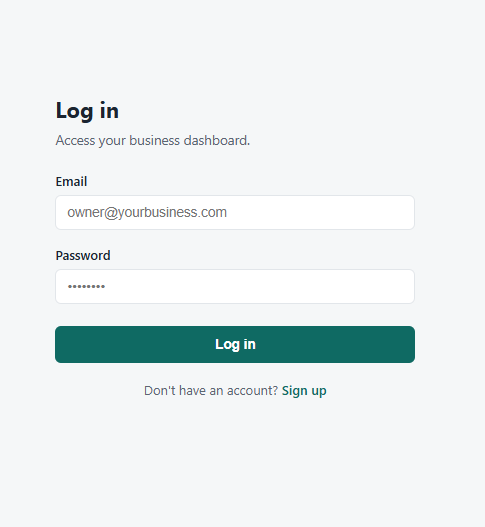
\includegraphics[width=0.75\linewidth]{Figures/login.png}
\caption{Login Page}
\end{figure}
Any registered user, whether a business owner or a store manager, logs in from this page using their email and password.

\subsection{Signup Page}

\begin{figure}[H]
\centering
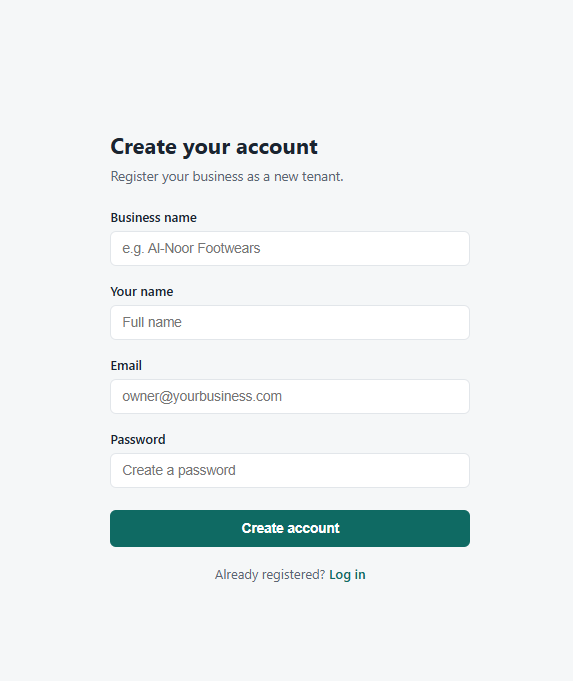
\includegraphics[width=0.75\linewidth]{Figures/signup.png}
\caption{Signup Page}
\end{figure}
A new business owner registers their business as a tenant from this page, creating the initial account for StockSense.

\subsection{Dashboard}

\begin{figure}[H]
\centering
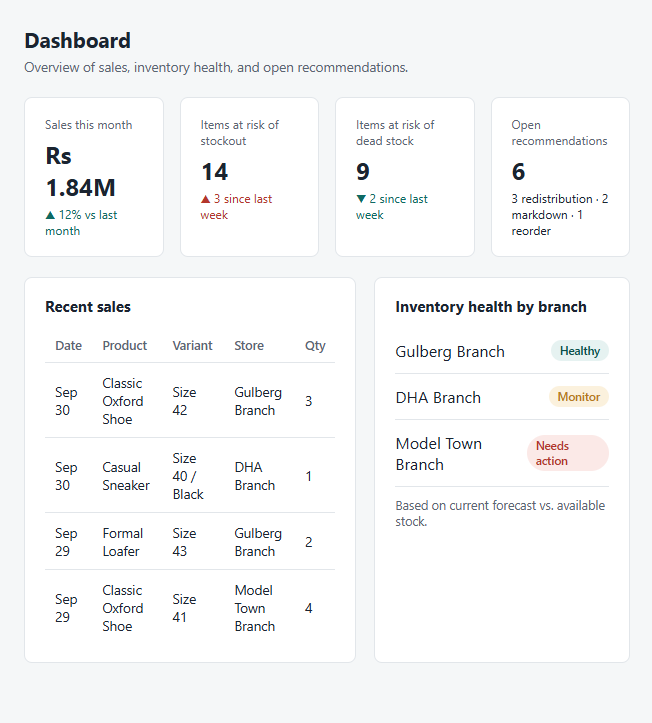
\includegraphics[width=0.9\linewidth]{Figures/dashboard.png}
\caption{Dashboard}
\end{figure}
On this page, the user can view an overview of monthly sales, items at risk of stockout or dead stock, recent sales activity, and inventory health across branches.

\subsection{Point of Sale}

\begin{figure}[H]
\centering
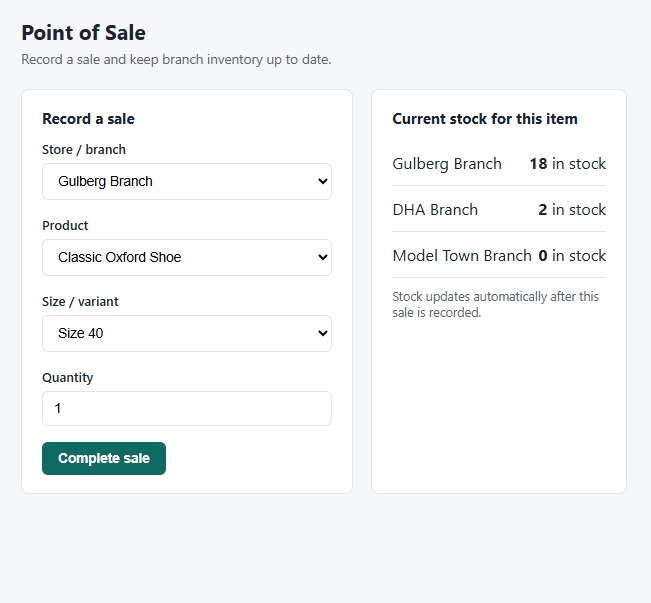
\includegraphics[width=0.9\linewidth]{Figures/pos.png}
\caption{Point of Sale}
\end{figure}
A store manager records a sale from this page by selecting the branch, product, and variant sold. Inventory is updated automatically once the sale is confirmed.

\subsection{Upload Sales Report}

\begin{figure}[H]
\centering
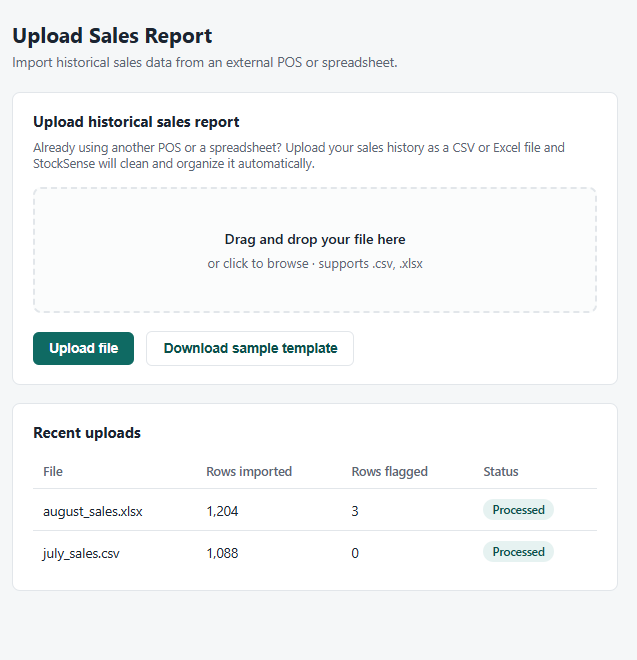
\includegraphics[width=0.9\linewidth]{Figures/upload.png}
\caption{Upload Sales Report}
\end{figure}
Businesses already using an external POS or spreadsheet can upload their historical sales data as a CSV or Excel file from this page, which is then validated and cleaned by the system.

\subsection{Inventory}

\begin{figure}[H]
\centering
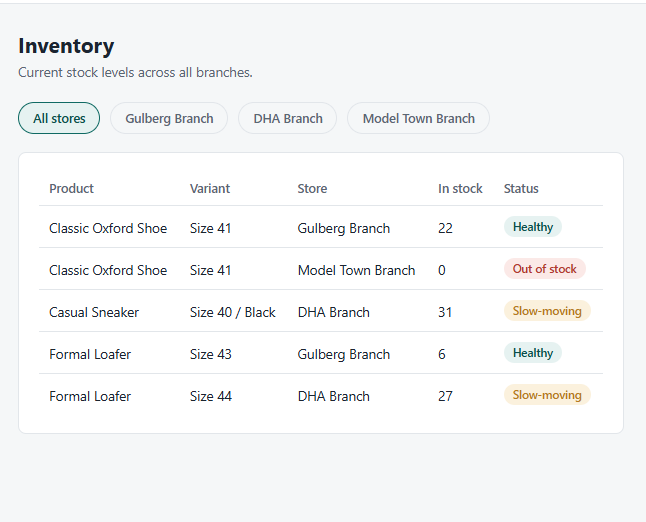
\includegraphics[width=0.9\linewidth]{Figures/inventory.png}
\caption{Inventory}
\end{figure}
This page displays current stock levels for every product variant across all branches, filterable by store, along with a status indicator for each item.

\subsection{Recommendations}

\begin{figure}[H]
\centering
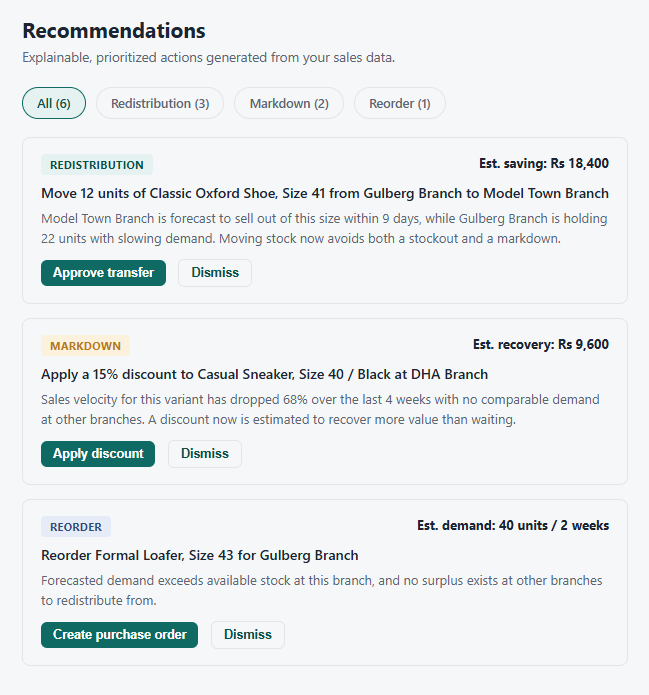
\includegraphics[width=0.9\linewidth]{Figures/recommendations.png}
\caption{Recommendations}
\end{figure}
This page lists the system's redistribution, markdown, and reorder recommendations, each with a plain-language explanation and an estimated financial impact, which the user can approve or dismiss.

\section{Database Design}

\subsection{ER Diagram}

\begin{figure}[H]
\centering
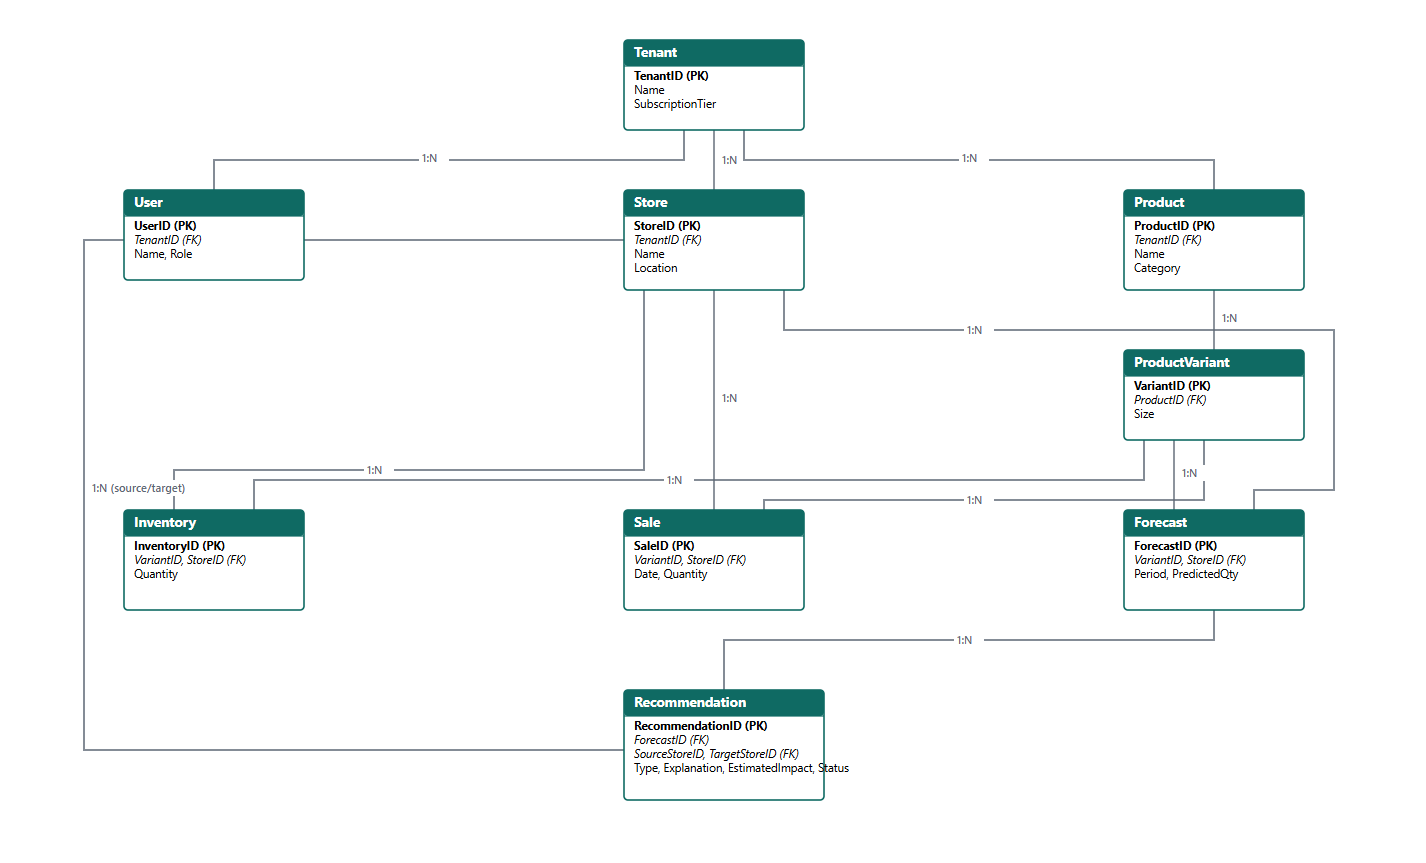
\includegraphics[width=\linewidth]{Figures/er_diagram.png}
\caption{ER Diagram}
\end{figure}

This is the design of the StockSense database. Each Tenant maintains separate Users, Stores, and Products, so that all business data is kept separate. A Product is associated with a number of Variants (e.g. sizes) and Inventory keeps track of how many of each Variant a Store has. Sales records and Forecasts are created at the Variant level per Store; Recommendations (redistribution, markdown, and reorder) are made based upon Forecasts and refer to the Store(s) involved.

The major entities and their relationships are:

\begin{itemize}
    \item A \textbf{Tenant} has many \textbf{Users}, \textbf{Stores}, and \textbf{Products}.
    \item A \textbf{Product} has many \textbf{Product Variants} (size/colour combinations).
    \item A \textbf{Store} maintains \textbf{Inventory} records per Product Variant.
    \item A \textbf{Sale} references a Product Variant, a Store, and a date/quantity.
    \item Historical \textbf{Sales} feed the \textbf{Forecast} entity, generated per Product Variant per Store.
    \item A \textbf{Forecast} is consumed by the \textbf{Recommendation} entity (redistribution, reorder, or markdown type).
\end{itemize}

\subsection{Data Dictionary}

\begin{table}[H]
\centering
\caption{Data Dictionary for Tenant Table}
\begin{tabular}{|l|l|p{6cm}|}
\hline
\textbf{Field} & \textbf{Type} & \textbf{Description} \\ \hline
TenantID & Integer & Unique identifier for each business \\ \hline
Name & String & Business name \\ \hline
SubscriptionTier & String & Free or Paid \\ \hline
CreatedDate & Date & Date the tenant registered \\ \hline
\end{tabular}
\end{table}

\begin{table}[H]
\centering
\caption{Data Dictionary for Store Table}
\begin{tabular}{|l|l|p{6cm}|}
\hline
\textbf{Field} & \textbf{Type} & \textbf{Description} \\ \hline
StoreID & Integer & Unique identifier for each store \\ \hline
TenantID & Integer & Owning tenant \\ \hline
Name & String & Store/branch name \\ \hline
Location & String & Store address or region \\ \hline
\end{tabular}
\end{table}

\begin{table}[H]
\centering
\caption{Data Dictionary for Product Variant Table}
\begin{tabular}{|l|l|p{6cm}|}
\hline
\textbf{Field} & \textbf{Type} & \textbf{Description} \\ \hline
VariantID & Integer & Unique identifier for a product-size combination \\ \hline
ProductID & Integer & Parent product \\ \hline
Size & String & Size or variant label \\ \hline
Category & String & Product category \\ \hline
\end{tabular}
\end{table}

\begin{table}[H]
\centering
\caption{Data Dictionary for Sale Table}
\begin{tabular}{|l|l|p{6cm}|}
\hline
\textbf{Field} & \textbf{Type} & \textbf{Description} \\ \hline
SaleID & Integer & Unique identifier for each sale \\ \hline
VariantID & Integer & Product variant sold \\ \hline
StoreID & Integer & Store where the sale occurred \\ \hline
Date & Date & Date of sale \\ \hline
Quantity & Integer & Units sold \\ \hline
\end{tabular}
\end{table}

\begin{table}[H]
\centering
\caption{Data Dictionary for Recommendation Table}
\begin{tabular}{|l|l|p{6cm}|}
\hline
\textbf{Field} & \textbf{Type} & \textbf{Description} \\ \hline
RecommendationID & Integer & Unique identifier for each recommendation \\ \hline
Type & String & Redistribution, Reorder, or Markdown \\ \hline
VariantID & Integer & Product variant involved \\ \hline
SourceStoreID & Integer & Store with surplus (redistribution only) \\ \hline
TargetStoreID & Integer & Store with forecasted need \\ \hline
Explanation & String & Plain-language reasoning for the recommendation \\ \hline
EstimatedImpact & Float & Estimated financial impact \\ \hline
Status & String & Pending, Actioned, or Dismissed \\ \hline
\end{tabular}
\end{table}

\section{Risk Analysis}

\begin{itemize}
    \item \textbf{Technical Risk:} Forecast accuracy may be poor for tenants with very limited historical sales data.
    \item \textbf{Data-Quality Risk:} Inconsistent or incomplete uploaded sales reports may require significant cleaning effort.
    \item \textbf{Adoption Risk:} Small-business owners may be reluctant to trust automated recommendations without a visible track record.
    \item \textbf{Scalability Risk:} As more tenants and historical data accumulate, forecasting jobs must remain performant.
    \item \textbf{Business Risk:} Changing project requirements or limited availability of real business data for testing.
\end{itemize}

\section{Conclusion}

In this chapter, you learned the functionality and non-functional requirements, use cases, and database design of StockSense. Requirements focus on three pillars identified in the Project Vision and Literature Review: affordable multi-tenant data collection using a free POS, product-size-location demand forecasting based on the literature for model selection, and explainable recommendations that focus on redistribution. The next chapter describes the proposed approach and methodology used to implement these requirements.

% ============================================================
% CHAPTER 5
% ============================================================

\chapter{Proposed Approach and Methodology}
\label{ch:methodology}

The proposed approach and methodology is presented in this chapter. The chapter explains how StockSense transforms raw sales data into inventory recommendations. It traces the data from ingestion to validation, construction of the demand series, forecasting, recommendation, optimization of markdowns, explanation, and evaluation. The literature reviewed in Chapter~3 is the basis for each design decision.

%==================================================
\section{Overall Pipeline}
\label{sec:pipeline}

StockSense is a sequential pipeline in which each stage reads data from and writes data to the PostgreSQL database through the modules described in Chapter~6. Sales are entered through the built-in POS or by file upload and are stored in one canonical schema. A demand series is created for each product-size-store combination, features are created from the history of the demand series, and the model provides weekly and monthly demand forecasts. These forecasts are then compared with the current inventory to generate redistribution, markdown, and reorder recommendations, all of which include an explanation and an estimated financial impact.

Forecasting and recommendation run as scheduled background jobs, and their results are stored in the Forecast and Recommendation tables. The model name (\texttt{ModelName}) is saved with each forecast, which allows models to be compared or replaced without altering the remainder of the system. To respect tenant isolation, models are trained per tenant: a model is shared across all products, sizes, and stores of one business, but never across businesses.

%==================================================
\section{Data Ingestion}
\label{sec:ingestion}

Sales come from two sources: \texttt{Sale} and \texttt{SaleItem} records from the built-in POS (Source = POS), and CSV or Excel files from an external system (Source = Upload). Both sources use the same schema, so the later stages are independent of the source.

Files are read with pandas (\texttt{read\_csv}, or \texttt{read\_excel} with \texttt{openpyxl}), in chunks to keep memory bounded for files of up to 100,000 rows. The system displays the detected columns, and the owner maps them to the canonical fields (product, size, store, date, quantity). Validation and import run as a background job. Validated rows are held until the owner approves the upload report, and are then committed in a single transaction. If the import fails, the transaction is rolled back and the data remains as it was before the import.

%==================================================
\section{Data Validation, Cleaning, and Normalization}
\label{sec:validation}

The following checks are performed for every row:

\begin{itemize}
    \item \textbf{Structural:} all required fields are present and have the expected data type.
    \item \textbf{Value:} the date is valid, the quantity is numeric, and the price is non-negative. Dates such as 03/04/2025 are ambiguous, so the owner selects the date format when the columns are mapped.
    \item \textbf{Referential:} product, size, and store names are normalized (trimmed, case folded, and sizes converted to a standard form such as ``Medium'' to ``M'') and must match a variant and a store within the same tenant. Unmatched rows are rejected with a reason, and close matches can be suggested using string similarity.
    \item \textbf{Duplicates:} rows repeated across overlapping exports are detected using a composite key (store, variant, date, quantity, price). They are flagged and not deleted, because identical sales can be genuine.
    \item \textbf{Returns and outliers:} negative quantities are treated as returns and reported separately. Extreme quantities are flagged and capped only in the training copy, so the raw record is preserved.
\end{itemize}

Accepted rows are stored in the canonical format. Rejected and flagged rows are listed in the upload report with reasons, allowing the owner to correct the source file.

%==================================================
\section{Demand Series Construction}
\label{sec:series}

Cleaned sales data are aggregated to the product-size-store level on a weekly and monthly basis:
\begin{equation}
    y(v,s,t) = \sum_{i \in \mathcal{S}(v,s,t)} q_i,
\end{equation}
where $\mathcal{S}(v,s,t)$ is the set of sale items of variant $v$ in store $s$ during period $t$, and $q_i$ is the quantity of sale item $i$.

A period without sales is treated as zero demand only from the date on which the variant was first stocked in that store, because demand before that date is unknown, not zero.

Size-level series are sparse and intermittent. Each series is therefore classified using the Syntetos--Boylan scheme, based on the average inter-demand interval (ADI) and the squared coefficient of variation of non-zero demand ($\mathrm{CV}^2$), as smooth, erratic, intermittent, or lumpy (commonly with thresholds $\mathrm{ADI}=1.32$ and $\mathrm{CV}^2=0.49$). This helps determine which baseline methods are used and makes it possible to report accuracy by demand type.

During a stock-out, observed sales underestimate demand. If stock history is available, weeks in which the variant was unavailable for most of the week are marked as censored and given zero weight in the training loss, instead of being learned as true zero demand.

%==================================================
\section{Feature Engineering}
\label{sec:features}

Each training example describes one variant in one store at a forecast origin $t$, with the demand at $t+h$ as the target. The feature groups are:

\begin{itemize}
    \item \textbf{Lag features:} demand at lags of 1 to 8 weeks, and at 52 weeks if at least one year of history exists (recent level, yearly seasonality).
    \item \textbf{Rolling statistics:} mean, standard deviation, and share of zero-sale weeks over the past 4, 8, and 12 weeks (level, volatility, intermittency).
    \item \textbf{Calendar features:} week of year, month, and holiday and festival indicators (seasonality, events).
    \item \textbf{Price features:} selling price, discount depth, and price relative to the category average (price effect).
    \item \textbf{Product and store attributes:} category, size, colour, store, and city, used as categorical features (sharing patterns across similar series).
    \item \textbf{Lifecycle features:} weeks since first sale and weeks since last sale (product age).
\end{itemize}

To prevent data leakage, features at origin $t$ use only data available up to $t$. Only features that are known in advance, such as calendar events, may refer to the future.

%==================================================
\section{Demand Forecasting Model}
\label{sec:forecasting}

\subsection{Global Gradient-Boosted Model}

The individual size-level series are too short and sparse to support one model per series. Following the global models of Montero-Manso and Hyndman and the forecasting of groups of similar series by Bandara et al., StockSense builds one global model per tenant on all of its series, with product, size, and store as categorical features. The chosen model is LightGBM (gradient-boosted decision trees). Gradient-boosted trees outperformed statistical methods on hierarchical retail sales in the M5 competition (Makridakis et al.), and LightGBM handles missing values and categorical variables natively and trains quickly on tabular data.

\subsection{Loss Function and Forecast Horizon}

Demand is non-negative and contains many zeros, so squared error is not a suitable loss. The model uses the Tweedie objective (power between 1 and 2), which models a point mass at zero together with a positive continuous part. The Poisson objective and squared error are retained as alternatives and compared experimentally.

Multi-step forecasts use a direct approach: a separate model is trained for each step $h = 1,\dots,H$ of the forecast horizon, so errors do not accumulate through recursive predictions:
\begin{equation}
    \hat{y}(v,s,t+h) = f_h\big(\mathbf{x}_{v,s,t}\big),
\end{equation}
where $\mathbf{x}_{v,s,t}$ denotes the features of variant $v$ in store $s$ at time $t$.

\subsection{Training and Tuning}

The hyperparameters (number of leaves, learning rate, minimum data per leaf, feature fraction, bagging fraction, and boosting rounds) are tuned with rolling-origin validation, using an expanding training window and early stopping on each fold. Random shuffling is never used, because it would expose future data to the model. Sample weights exclude censored periods from the loss.

\subsection{Statistical Baselines}

To evaluate whether the more complex model is necessary, the following baselines are computed on the same splits: the naive forecast (last value), the seasonal naive forecast (with at least one year of history), the moving average, Holt--Winters exponential smoothing (\texttt{statsmodels}), and Croston's method for intermittent series.

\subsection{Initial Training Period}

StockSense does not ship with a pre-trained model, and the data of one tenant is never shared with another. A new tenant therefore starts without a forecasting model. The owner first records sales through the POS or uploads historical sales reports. Until a minimum amount of history is available (for example, several weeks of sales for the tenant's products), no forecast is displayed and the user is told that more data is needed (UC-10). Once the minimum is reached, the first model is trained on the tenant's own data, and forecasting and recommendations start working. The model is then retrained on a schedule as new sales arrive, so its accuracy improves as the tenant's history grows. The minimum history is determined experimentally (Section~\ref{sec:evaluation}).

\subsection{Forecast Uncertainty}

In addition to the point forecast, an upper-quantile forecast (for example, the 0.9 quantile using the quantile objective of LightGBM) is trained. The recommendation engine uses it to establish safety stock, so that decisions account for uncertainty and not only the mean.

%==================================================
\section{Recommendation Engine and Stock Redistribution}
\label{sec:recommendation}

For every variant $v$ and store $s$, the engine compares the forecast with the stock position over a planning horizon of $H$ weeks. Define:

\begin{itemize}
    \item $I$ = on-hand stock plus pending incoming transfers (pending transfers are already accepted, so they are not recommended again),
    \item $D$ = forecast demand over the next $H$ weeks,
    \item $SS$ = safety stock, taken from the upper-quantile forecast.
\end{itemize}

The net position is
\begin{equation}
    N = I - (D + SS).
\end{equation}
If $N > 0$, the store has a surplus of $N$ units; if $N < 0$, it has a shortage of $-N$ units.

\textbf{Redistribution.} Following the proactive-transshipment approach of Paterson et al., transfers are planned before a stock-out or dead stock occurs. For each variant, the transfer quantities $x_{ij}$ from surplus store $i$ to shortage store $j$ are obtained by solving a transportation problem:
\begin{align}
    \max_{x}\quad & \sum_{i}\sum_{j} \big(m - c_{ij}\big)\, x_{ij} \\
    \text{s.t.}\quad & \sum_{j} x_{ij} \le \text{surplus}_i \quad \forall i, \\
    & \sum_{i} x_{ij} \le \text{shortage}_j \quad \forall j, \\
    & x_{ij} \ge 0.
\end{align}
Here $m$ is the unit margin (selling price minus cost price) and $c_{ij}$ is the unit transfer cost between stores $i$ and $j$. A transfer is recommended only if $m > c_{ij}$. The constraint matrix of a transportation problem is totally unimodular, so the LP solution is automatically integral, and since retailers have few branches, each problem is small and cheap to solve.

\textbf{Reorder.} Any shortage remaining after redistribution is converted into a reorder recommendation with a suggested quantity.

\textbf{Priority.} Recommendations are processed in the order redistribution, markdown, reorder, because moving existing stock is usually easier and less costly than discounting or reordering.

%==================================================
\section{Markdown Optimization}
\label{sec:markdown}

Any surplus that is not cleared by redistribution is passed to the markdown optimizer. Like Caro and Gallien, it follows a forecast-then-optimize structure, but it is used as an early-warning mechanism rather than an end-of-season clearance approach.

A variant-store is marked as at risk when its weeks of cover exceed the remaining selling window:
\begin{equation}
    \mathrm{WOC} = \frac{I}{\bar{d}} > T,
\end{equation}
where $\bar{d}$ is the average forecast weekly demand and $T$ is the number of weeks in which the stock should be sold. Because the alert is raised while WOC is only slightly above $T$, a small discount is usually sufficient.

For each candidate discount $d$ from a grid (for example, 5\% to 50\% in steps of 5\%), demand is adjusted using a constant price-elasticity model:
\begin{equation}
    D(d) = D \cdot (1 - d)^{-\varepsilon}, \qquad
    \text{Sold}(d) = \min\big(I,\; D(d)\big),
\end{equation}
where $D(d)$ is the total adjusted demand over the horizon.

The system recommends the smallest discount for which the projected sell-through reaches a target, subject to a margin floor $p\,(1-d) \ge c$, where $p$ is the selling price and $c$ is the cost price. The estimated impact is the difference in margin with and without the discount:
\begin{equation}
    \text{Impact} = \text{Sold}(d)\,\big(p(1-d) - c\big) - \text{Sold}(0)\,\big(p - c\big).
\end{equation}

The elasticity $\varepsilon$ is estimated by log-log regression on the tenant's own price history when there is sufficient price variation. Otherwise, a conservative category-level default is used, and the recommendation states that the estimate is approximate.

%==================================================
\section{Explainable Recommendations}
\label{sec:explain}

Every recommendation is stored together with a two-part explanation:

\begin{itemize}
    \item A structured record of the quantities involved in the decision: forecast demand, current stock, net position, weeks of cover, source and destination stores, margin, transfer cost, and estimated impact.
    \item The main forecast drivers, extracted from the per-feature contributions of LightGBM (\texttt{pred\_contrib}, additive SHAP-style values) and rendered as plain phrases such as ``recent weekly sales'' or ``seasonal pattern''.
\end{itemize}

Both parts are filled into text templates, for example: ``Size M of this product is expected to sell 12 units at Store B in the next 4 weeks, but only 3 are in stock, while Store A holds 15 units that are expected to sell only 4.'' The explanation is saved at creation time, so it always shows the situation on which the recommendation was based.

%==================================================
\section{Forecast and Recommendation Evaluation}
\label{sec:evaluation}

\subsection{Data}

Public retail datasets are used for initial development and validation. A dataset such as M5 contains store-item sales and prices, which supports evaluation at the store level and the hierarchy level, but it does not contain size-level sales. Size-level behaviour is therefore evaluated on real retailer sales data if access is secured, and the findings from public data are interpreted with this limitation in mind, as stated in Chapter~2.

\subsection{Protocol}

All splits are chronological. Hyperparameters are tuned with rolling-origin validation, and the final comparison is made on the most recent period, which the models never see during training or tuning.

\subsection{Metrics}

The primary metrics are
\begin{align}
    \mathrm{RMSE} &= \sqrt{\frac{1}{n}\sum_{k=1}^{n}\big(a_k - f_k\big)^2}, \\
    \mathrm{MAPE} &= \frac{100}{|P|}\sum_{k \in P}\frac{|a_k - f_k|}{a_k}, \qquad P = \{k : a_k > 0\},
\end{align}
where $a_k$ is the actual demand and $f_k$ is the forecast.

Size-level series contain many zeros and MAPE is undefined for zero actuals, so it is computed only on non-zero periods and always reported together with RMSE. WAPE (total absolute error divided by total actual sales) and MAE are provided as supplementary measures, since they remain valid for sparse series. Results are presented separately for each demand class, for fast and slow movers.

\subsection{Experiments}

\begin{itemize}
    \item LightGBM against the statistical baselines (the main claim of Chapter~3).
    \item The global model against separate models for each series.
    \item Forecast accuracy against the amount of training history available (for example, 4, 8, and 12 weeks), to estimate how much data a new tenant must provide before forecasts become reliable.
    \item Tweedie and Poisson objectives against squared error.
\end{itemize}

\subsection{Recommendation Backtest}

The value of the recommendations is estimated by replaying history. At each cut-off date, the engine produces recommendations using only the information available up to that date. The recommended transfers and discounts are applied to a simulated stock record, and the following weeks are replayed with actual sales as demand. The outcomes are compared with a ``no action'' run and include dead stock (units whose cover is greater than $T$ weeks), units of lost sales caused by stock-outs, and the sell-through rate. The simulation assumes that transfers do not change demand, and that demand changes only through the elasticity model when a markdown is applied. These assumptions are stated together with the results.

%==================================================
\section{Iterative Development}
\label{sec:iterative}

StockSense is built in increments, and each increment ends with the tests in Section~6.7 and a review by the supervisor:

\begin{enumerate}
    \item \textbf{Multi-tenant foundation:} tenant and user management, products, inventory, POS, and the ingestion and validation pipeline.
    \item \textbf{Forecasting experiments} in Jupyter Notebook: feature engineering, baselines, and LightGBM, all evaluated offline.
    \item \textbf{Integration:} scheduled batch forecasting, the recommendation engine, and redistribution.
    \item \textbf{Markdown optimization,} explanations, notifications, and the dashboard.
\end{enumerate}

Building the forecasting models offline first allows the choice of model to be checked on data before integration.

%==================================================
\section{Conclusion}
\label{sec:conclusion}

The methodology treats each sale as the beginning of a decision path. Data is validated and standardized, and demand is modelled at the product-size-store level using a global LightGBM model that is compared against statistical baselines. A new tenant first provides sales data so that a model can be trained on its own history, after which forecasting starts. The recommendation engine then transforms forecasts into actions in a fixed order: redistribution through a small transportation problem, early markdown through a sell-through model, and finally reorder for the remaining shortage. Every recommendation includes an explanation and an estimate of its impact. The evaluation uses chronological splits and a replay of past data, so that both forecast accuracy and the potential reduction of dead stock can be measured.


% ============================================================
% CHAPTER 6
% ============================================================

\chapter{High-Level and Low-Level Design}

\section{System Overview}

StockSense is a multi-tenant SaaS solution for small and medium-sized retailers to minimise dead stock and stock out in their stores, leveraging their own sales data. Every business is an independent tenant and has its own users, stores, products, inventory and sales. The sales are made using the built-in POS system or via CSV/Excel files which can be uploaded. The system predicts demand at product-size-store level and suggests actions with an accompanying clear explanation on a single web dashboard. These will be the modules that will be incorporated into our system:

\subsection{Tenant and User Management}

This module processes the registration of a business, user logon and roles. Ensures that an owner, store manager and/or administrator can only access information for which they have the authority and tenant.

\subsection{POS and Inventory Management}

This module is the free part of StockSense. It records sales and keeps the current stock of every product, size, and store up to date.

\subsection{Data Ingestion and Cleaning}

This module imports historical sales data from CSV or Excel files, validates the data, identifies the invalid records and formats the data into a consistent standard format. It allows businesses that already have a point of sale or spreadsheet to participate without having to change their system.

\subsection{Demand Forecasting}

This module forecasts the weekly and monthly demand of each product, size and store. It trains a model on each tenant's own sales history, so a new tenant must first record or upload enough sales data before forecasts are shown.

\subsection{Stock Redistribution and Reorder Recommendations}

This module is a comparison of the forecast and the current stock of each branch. It recommends moving stock from a branch with more stock to one with less stock first and suggests a reorder only if the amount of stock is insufficient being moved.

\subsection{Markdown Optimization}

The module identifies slow moving stock and suggests selling the stock at an early stage prior to it being dead.

\subsection{Explainable Recommendations}

Each recommendation is accompanied by a brief description of why it is recommended, and an approximate financial impact so the owner can comprehend and commit to the recommendation.

\subsection{Dashboard and Reporting}

This module displays the sales, inventory, forecasts, and recommendations to the Owner and the Store Managers in an easy to use web interface.

\section{Design Considerations}

This section lists the dependencies and limitations that affect the design of StockSense, so that they can be handled before the implementation starts.

\subsection{Assumptions and Dependencies}

\subsubsection{Operating System and Browser}

StockSense is a web application. Users must be running a relatively new version of Chrome, Edge, Firefox or Safari on their laptop, desktop or tablet.

\subsubsection{End User Characteristics}

\begin{itemize}
    \item Users have a stable internet connection.
    \item Owners/managers have not mastered computers but know some of the basic uses.
    \item The retailer can access historical sales data or can record new sales in the built-in, point-of-sale system.
\end{itemize}

\subsubsection{Possible Changes in Functionality}

The quality of forecasts depends on the quality and amount of sales data. During development, the functionality may change as a result of testing of the datasets and feedback from the supervisor. That is the intent of the modular design to facilitate such change.

\subsection{General Constraints}

\subsubsection{Hardware and Software Environment}

\begin{itemize}
    \item More computing power is required for forecasting and data processing (than for normal page requests).
    \item The interface needs to be compatible with various devices and browsers.
    \item There may be constraints on what we can do when implementing with external libraries or service.
\end{itemize}

\subsubsection{End-User Environment}

\begin{itemize}
    \item Slow or unstable internet in some shops.
    \item Many managers have no training in data analysis and the interface should not be technologic.
\end{itemize}

\subsubsection{Data Format Differences}

\begin{itemize}
    \item Uploaded files vary in column names, date formatting and product naming.
    \item All of them are to be converted to a single standard internal format.
\end{itemize}

\subsubsection{Data Repository and Tenant Isolation}

\begin{itemize}
    \item Never any one business should have access to another business data.
    \item All records should be associated with tenant.
    \item The database needs to expand to include additional tenants and additional sales history.
\end{itemize}

\subsubsection{Security Requirements}

\begin{itemize}
    \item It is user's responsibility to log in with their own username and password, and to keep their password protected.
    \item Access should be based on user role.
    \item Data needs to be safeguarded whilst in transit and whilst stored.
\end{itemize}

\subsubsection{Performance Requirements}

\begin{itemize}
    \item Forecasting and large uploads have to be performed in the background.
    \item The results with frequent use, like the latest forecasts, are stored and do not need to be calculated time and time again.
    \item Clearly error messages should be produced for invalid input.
\end{itemize}

\subsubsection{Interoperability Requirements}

\begin{itemize}
    \item The system needs to be able to import CSV and Excel files from external point-of-sales (POS) systems and spreadsheets.
    \item The internal modules should communicate using unambiguous interfaces.
\end{itemize}

\subsubsection{Verification and Validation Requirements}

\begin{itemize}
    \item It is important to test the upload pipeline with bad and garbled files.
    \item Tenant separation is necessary to be tested for data leakage.
    \item Predictions need to be judged against past data, as described in Chapter 5.
\end{itemize}

\subsection{Goals and Guidelines}

\subsubsection{The KISS Principle}

The design should be kept simple to make maintenance and non-technical user friendly.

\subsubsection{Separation of Tenant Data}

Each firm requires its very own safeguarded data room.

\subsubsection{Modularity and Extensibility}

Forecasting, recommendations, POS, ingestion, and markdown should be separated so as to allow the inclusion of new forecasting approaches without reengineering the system.

\subsubsection{Explainability}

All recommendations should include the rationale for the recommendation.

\subsection{Development Methods}

StockSense will be developed iteratively, in stages. Initial modules will include tenant management, product and inventory management and data ingestion, followed by forecasting, recommendations, markdown optimization and dashboard. An evaluation will be conducted for each stage prior to the beginning of the next stage and the plan will be modified based on feedback from the supervisor.

\section{System Architecture}

StockSense has a multi-layered web structure. The users interact with the web dashboard or the POS interface, which will communicate with the API in the back end. The API verifies the identity of the user, their tenant and passes the request to the appropriate module. The cleaned sales data feeds into a forecasting engine, while the forecasts are fed into a recommendation engine and the valid stock data from the POS and inventory module feeds into a recommendation engine. The slow moving stock is passed to the markdown optimizer. All the results are recorded in the database and displayed back to the user at the dashboard. The full picture is displayed in Figure~\ref{fig:system-architecture}.

\begin{figure}[H]
    \centering
    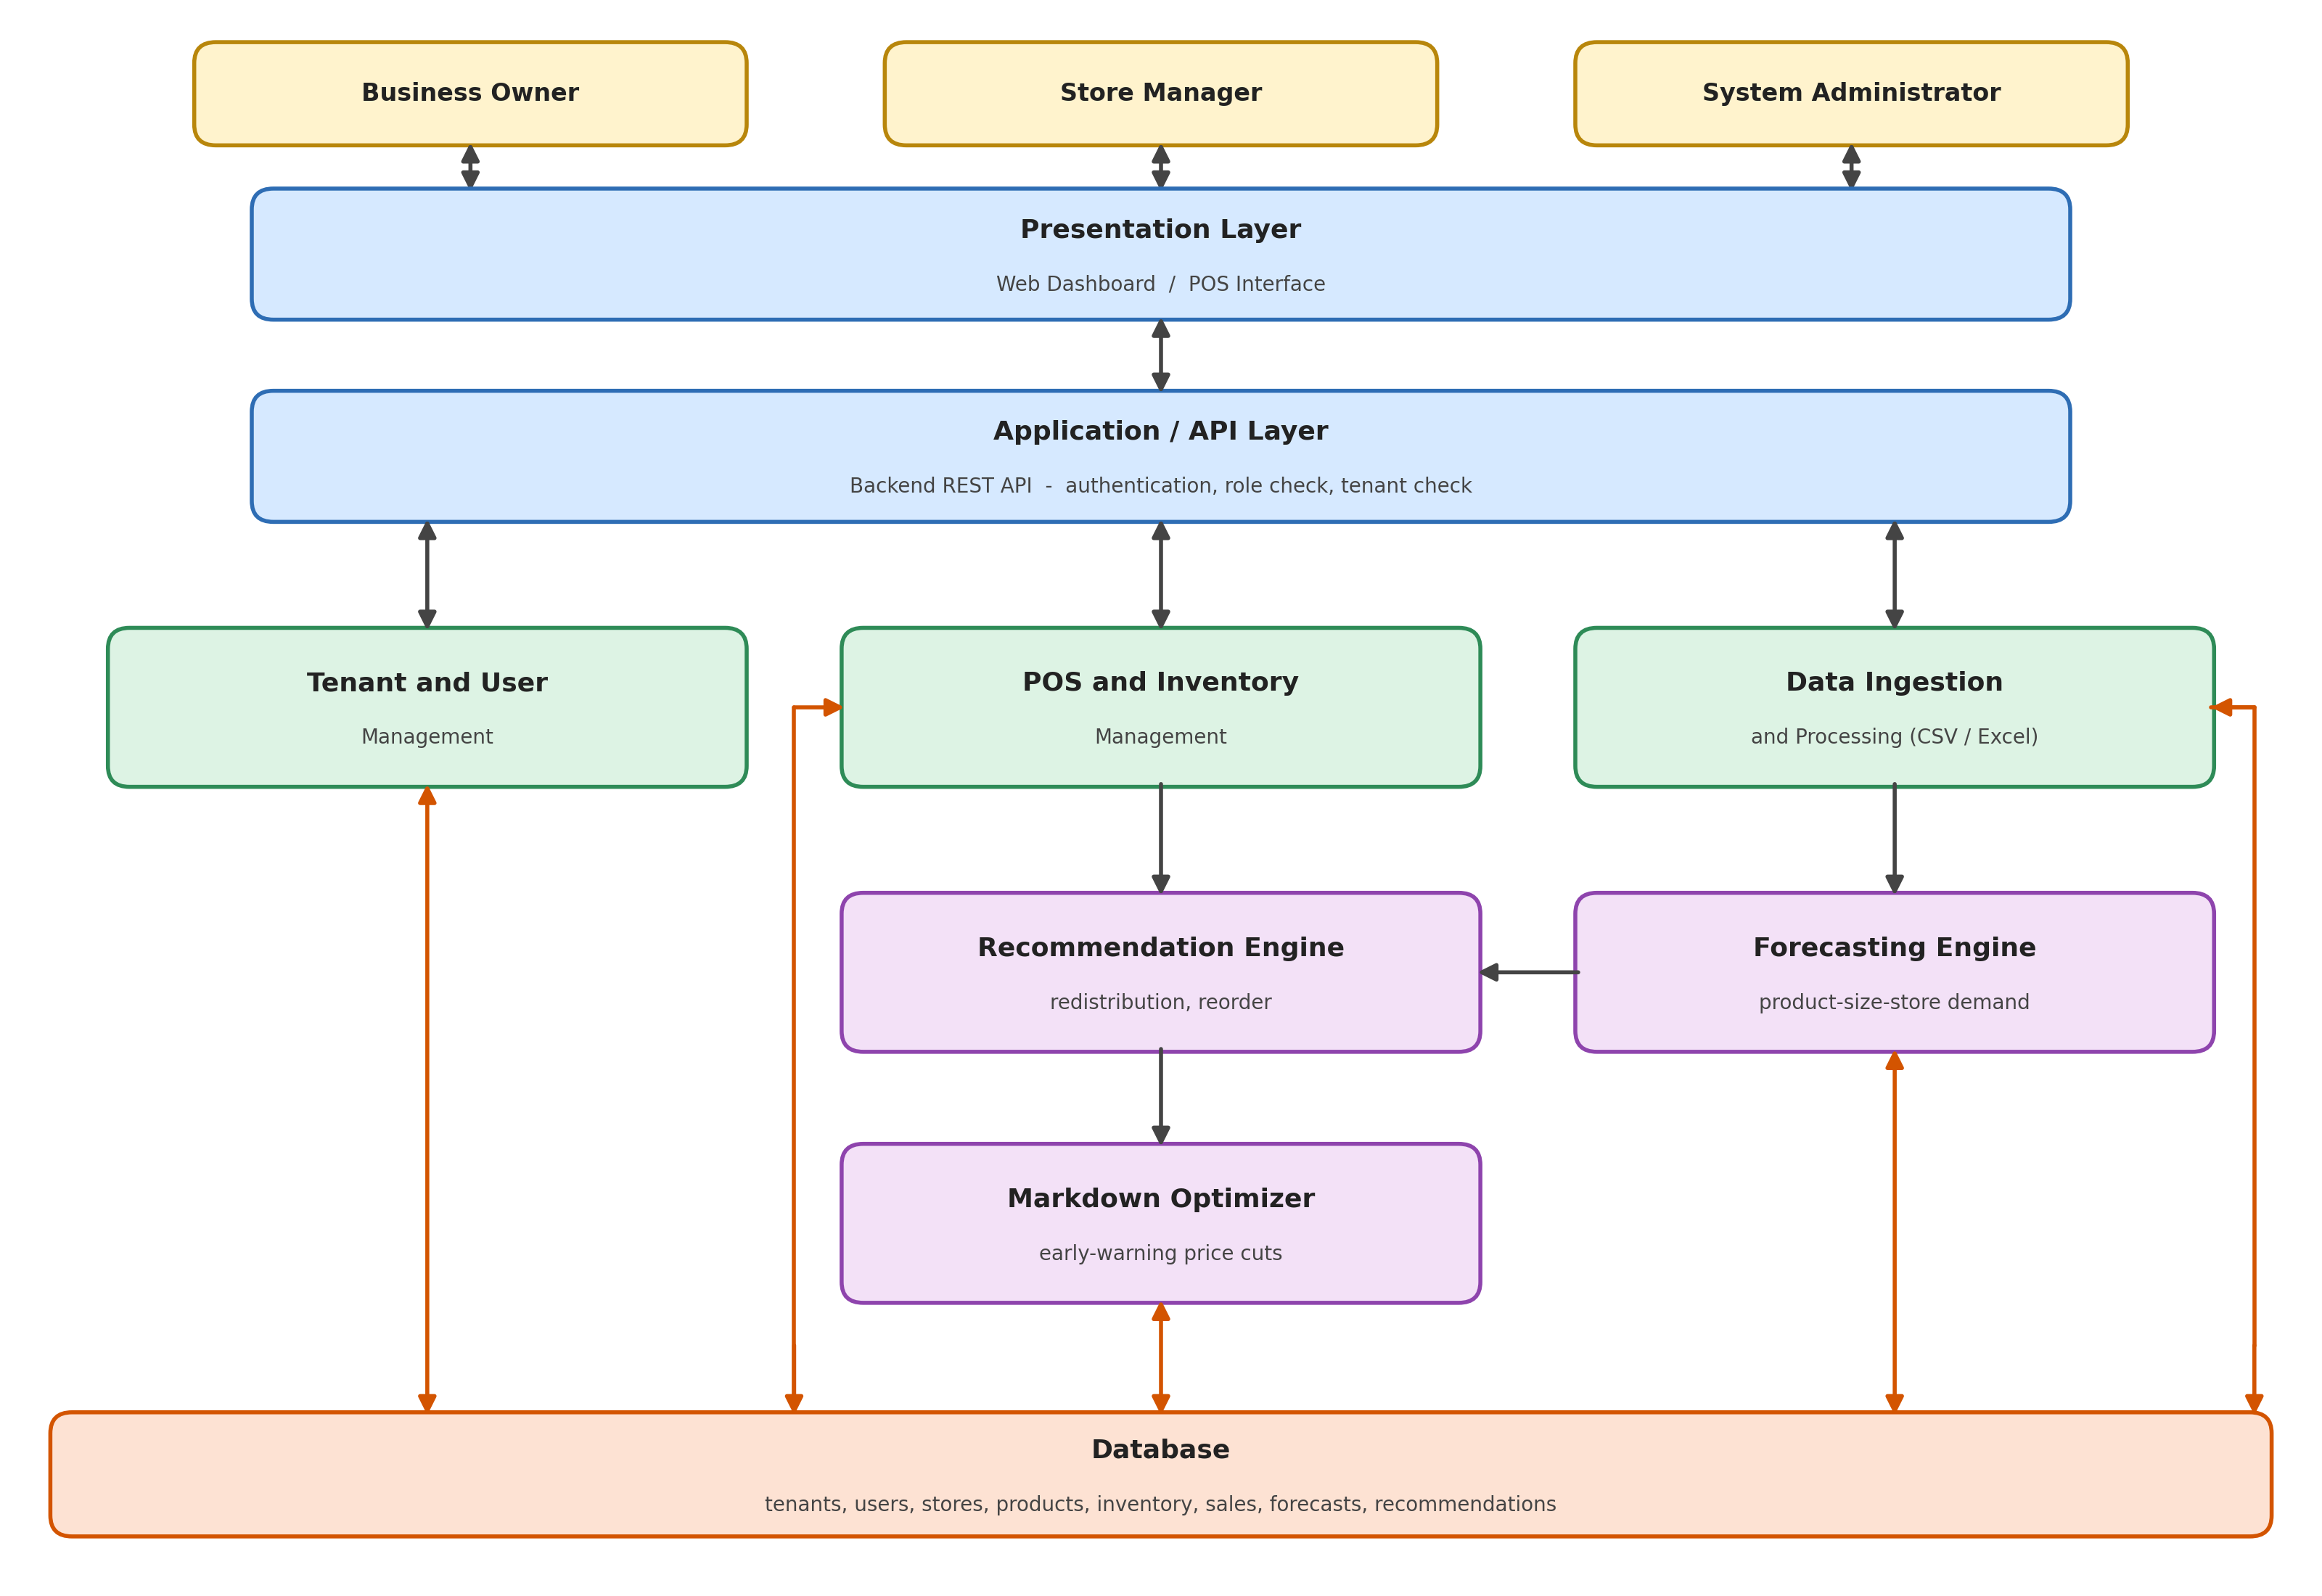
\includegraphics[width=\textwidth]{Figures/system_architecture.png}
    \caption[System Architecture Diagram]{System Architecture Diagram\\ This figure shows the System Architecture Diagram of our Application}
    \label{fig:system-architecture}
\end{figure}

\subsection{Subsystem Architecture}

\subsubsection{User and Tenant Management}

This subsystem contains business and business users. It supports roles, login and registration, and ensures that every user only has access to data from his/her tenant.

\subsubsection{POS and Inventory Subsystem}

This subsystem maintains the current item count for each item, size and store, and documents the total sales for each item, size, store.

\subsubsection{Data Ingestion Subsystem}

This subsystem is able to accept CSV and Excel files, validate them, flag invalid records and convert files to the standard format used internally.

\subsubsection{Forecasting Subsystem}

This subsystem analyzes the sales history of a tenant and forecasts the weekly and monthly demand at product-size-store level. It trains a model on the tenant's own data, and no forecast is shown until enough history has been recorded or uploaded.

\subsubsection{Recommendation Subsystem}

This subsystem is a comparison of forecasts with the level of each branch. It advises to move stock from one branch to another first, and then recommends a reorder when this is not sufficient. These recommendations along with the reason and estimated financial impact are stored with each recommendation.

\subsubsection{Markdown Optimization Subsystem}

This subsystem is looking for stock that is not selling fast enough and advises a reduction in price early enough that it can be sold.

\section{Architectural Strategies}

\subsection{Multi-Tenant Architecture}\label{sec:multitenant}

Many companies will share the same platform but the data will remain logically separate. All records that are important will have a tenant identifier on them, and all requests will be compared to it before reading or updating any data.

\subsection{Modular Architecture}

The modules will be forecasting, recommendations, POS, data ingestion, markdown optimization. If one of them changes (e.g. a new forecasting model), then the others should not need to change significantly.

\subsection{Programming Languages and Frameworks}

The web interface will be created using React. The backend REST API will be developed in python (FastAPI or Django), the main model for forecasting will be lightgbm, the statistical baseline will be statsmodels and pandas and openpyxl will be used for processing of csv and excel files.

\subsection{Database}

A PostgreSQL relational database will store all business data. Each table in a business has a business tenant identifier, which is helpful for tenant isolation covered in Section~\ref{sec:multitenant}. The detailed design will be provided in the database design part of chapter 4.

\subsection{Background Processing}

Forecasting and cleaning of large files may be time-consuming. These jobs will continue to run in the background and the user will be told when the results are available so the dashboard remains speedy.

\subsection{Error Detection and Recovery}

The system will record the following information regarding failed uploads, rejected records and failed forecasting runs to help identify the cause: In case a forecasting run is unsuccessful, previous valid forecasts will remain and not be eliminated from the forecasting dashboard.

\section{Domain Model/Class Diagram}

The domain model of StockSense is shown in Figure~\ref{fig:class-diagram}. It follows the data dictionary of Chapter~4: every business-owned class belongs to exactly one \textbf{Tenant}, and the foreign keys of the database are expressed as associations between classes.

The major classes of the system are:

\begin{itemize}
    \item \textbf{Tenant} and \textbf{Subscription}: a business on the platform and its free/paid plan history.
    \item \textbf{User}: Business Owner, Store Manager, or System Administrator (distinguished by the \texttt{role} attribute).
    \item \textbf{Store}: a branch of a business.
    \item \textbf{Product} and \textbf{ProductVariant}: a product and its sizes/variants, each with its own SKU.
    \item \textbf{Inventory}: the quantity of one variant held at one store.
    \item \textbf{Sale} and \textbf{SaleItem}: a customer sale (POS or uploaded) and the variants it contains.
    \item \textbf{UploadJob}: an uploaded CSV/Excel file with its accepted and rejected row counts.
    \item \textbf{Forecast}: the predicted demand of one variant at one store for a weekly or monthly period.
    \item \textbf{Recommendation} (abstract) with the subclasses \textbf{RedistributionRecommendation}, \textbf{ReorderRecommendation}, and \textbf{MarkdownRecommendation}.
    \item \textbf{StockTransfer}: the movement of stock between two stores, created when a redistribution recommendation is accepted.
    \item \textbf{Notification}: an alert sent to a user when a recommendation is raised.
\end{itemize}

The basic relationships between these classes are as follows:

\begin{itemize}
    \item A Tenant has one or more Subscriptions over time, and owns many Stores, Products, and UploadJobs.
    \item A Tenant has many Users; a System Administrator belongs to no Tenant.
    \item A Store Manager is assigned to a Store; a Store can have many Users assigned to it.
    \item A Product has one or more ProductVariants (sizes).
    \item Inventory links one ProductVariant to one Store with a quantity.
    \item A Sale occurs at one Store and contains one or more SaleItems; each SaleItem refers to one ProductVariant. A Sale may come from an UploadJob (null for POS sales).
    \item A Forecast is generated for one ProductVariant at one Store for a period.
    \item A Recommendation concerns one ProductVariant, refers to a source Store, and may be based on a Forecast. It is accepted or dismissed by a User.
    \item A RedistributionRecommendation also has a destination Store and, when accepted, triggers one StockTransfer between two Stores.
    \item A Notification is received by one User and may refer to a Recommendation.
\end{itemize}

\begin{figure}[H]
    \centering
    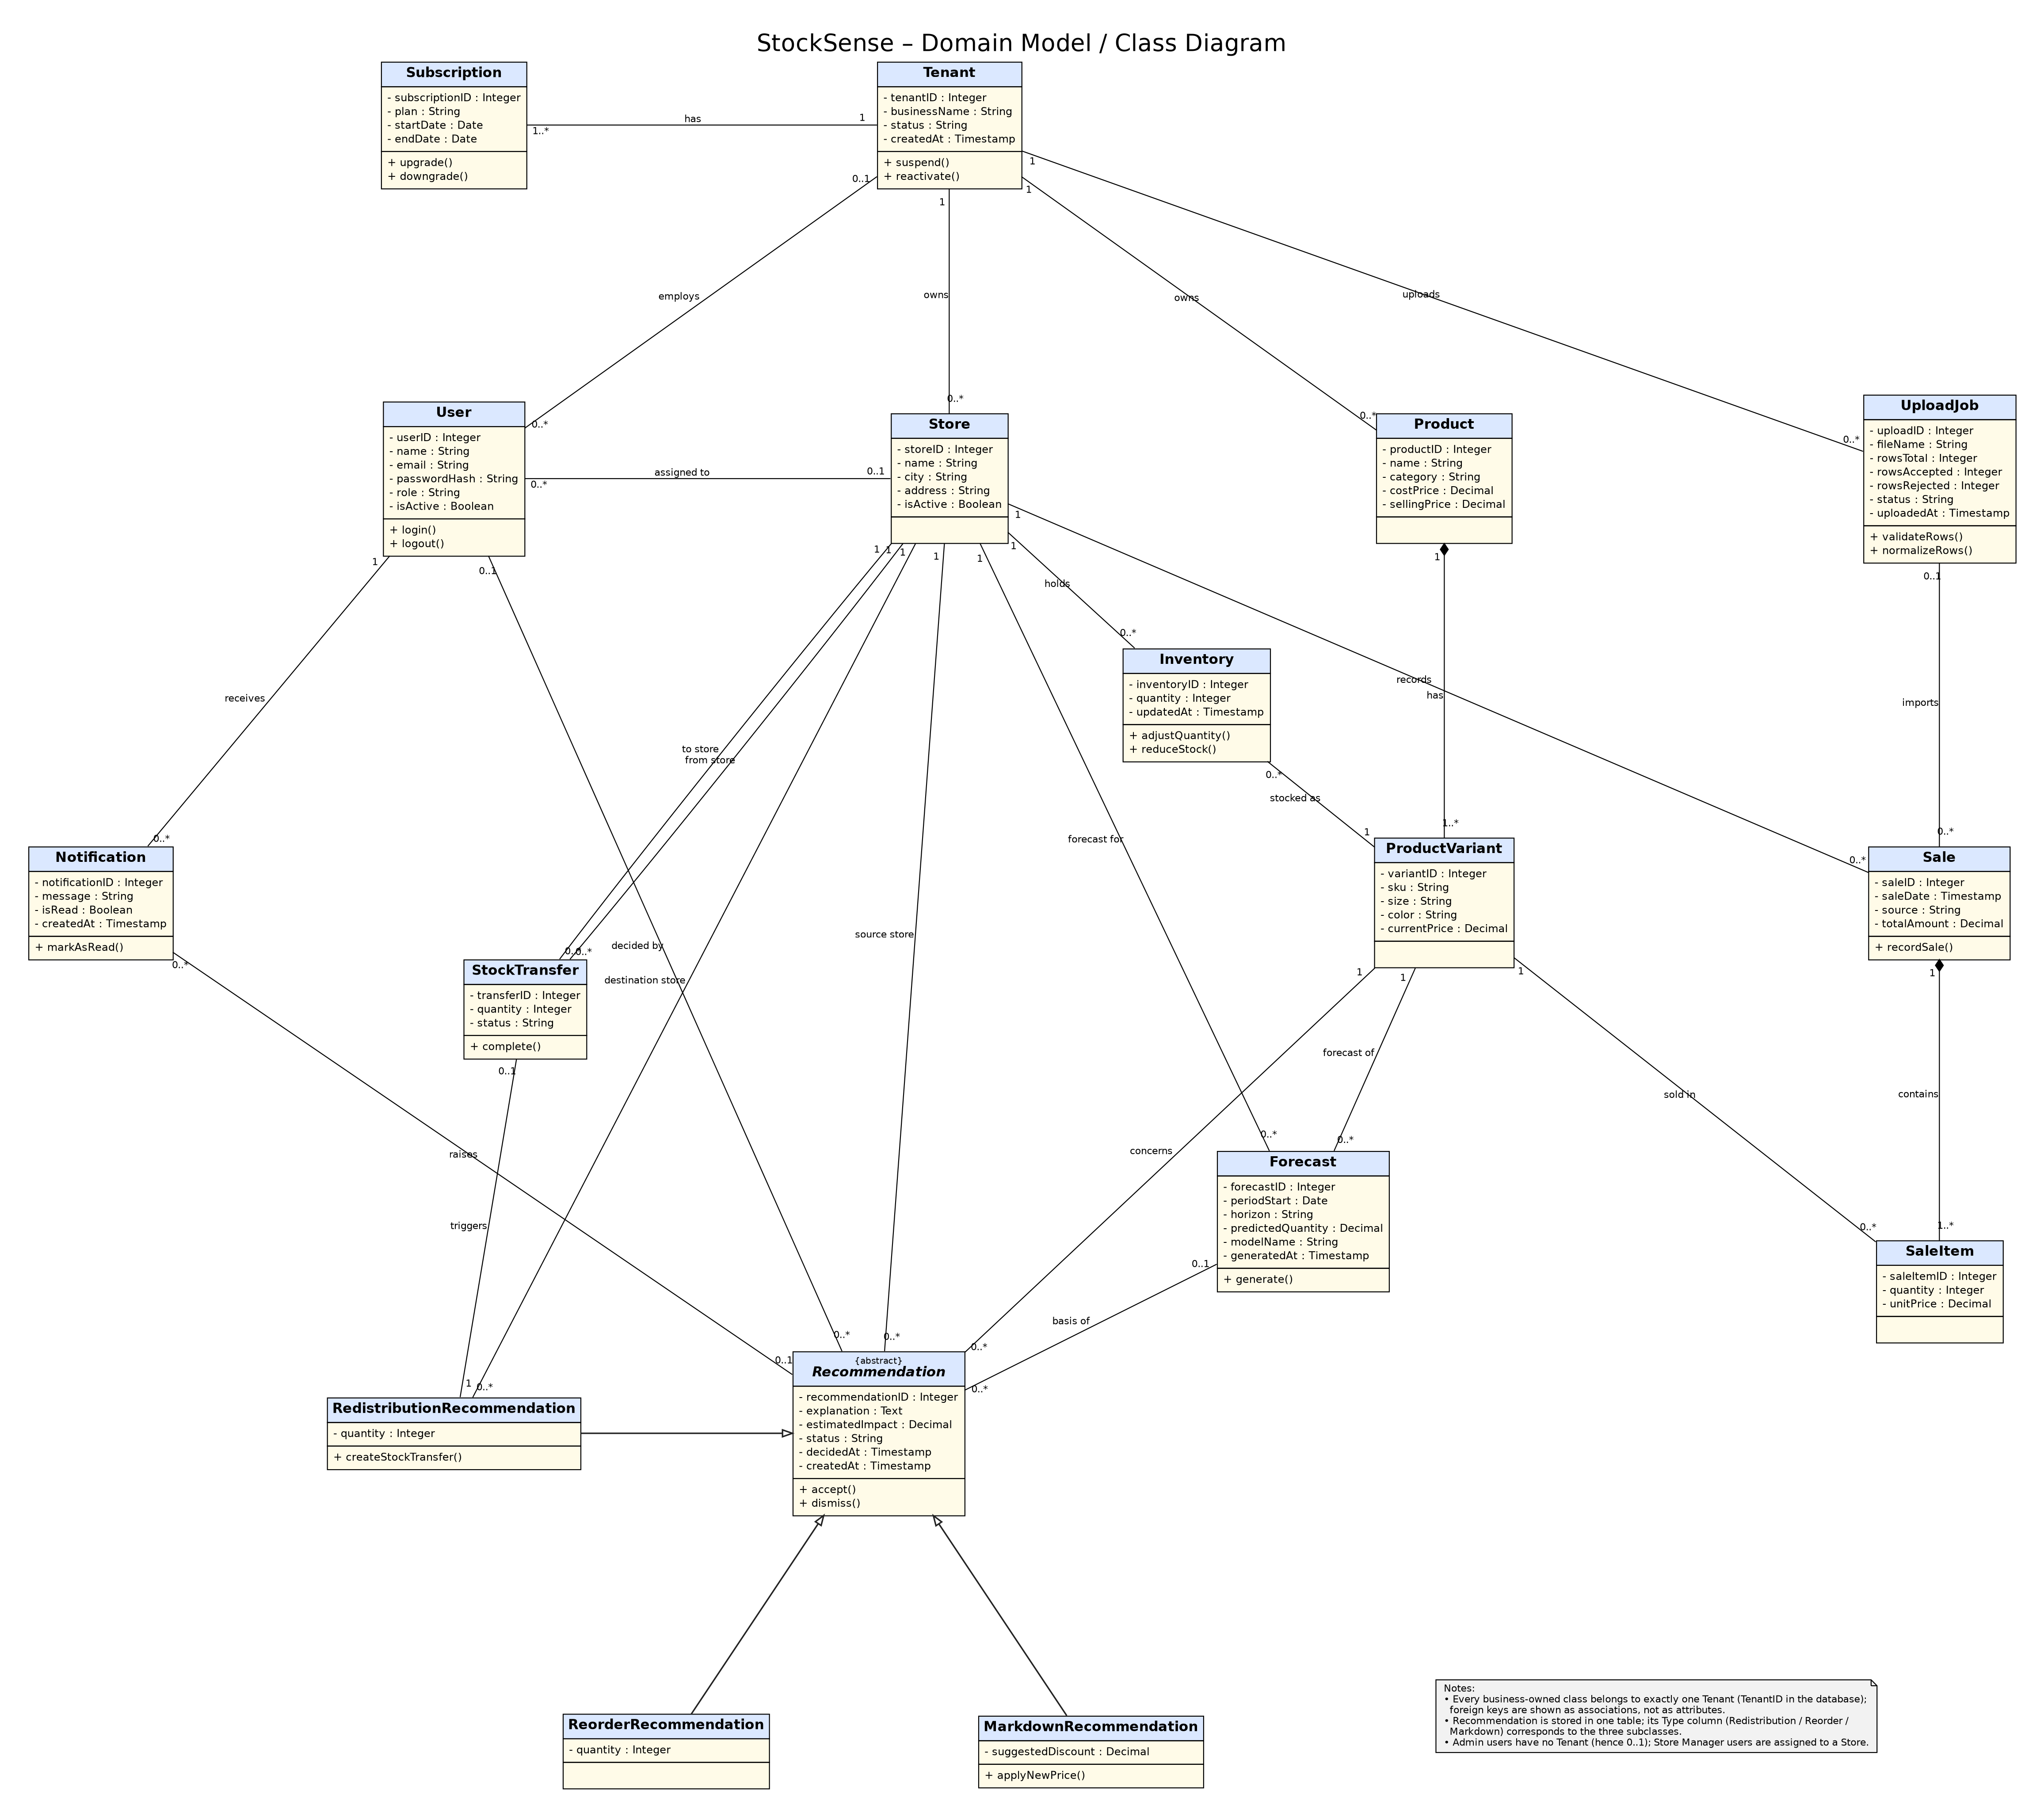
\includegraphics[width=\textwidth]{Figures/class_diagram.png}
    \caption[Domain Model / Class Diagram]{Domain Model / Class Diagram\\ This figure shows the Domain Model / Class Diagram of our Application}
    \label{fig:class-diagram}
\end{figure}

\section{Sequence Diagrams}
 
This section presents one sequence diagram for each use case described in Chapter~4. Each diagram shows the order of messages exchanged between the actor, the user interface, the application layer (API / controller or service), and the database for the basic flow of the use case. Alternative flows are drawn as \texttt{alt} fragments, optional behavior as \texttt{opt} fragments, repeated steps as \texttt{loop} fragments, and operations that must succeed or fail together as a single database transaction. Every request is restricted to the data of the user's tenant, as described in the multi-tenant architecture.
 
\subsection{UC-01: Register Business}
 
This diagram shows the interaction for the use case \textbf{Register Business} (UC-01).
 
\begin{figure}[H]
    \centering
    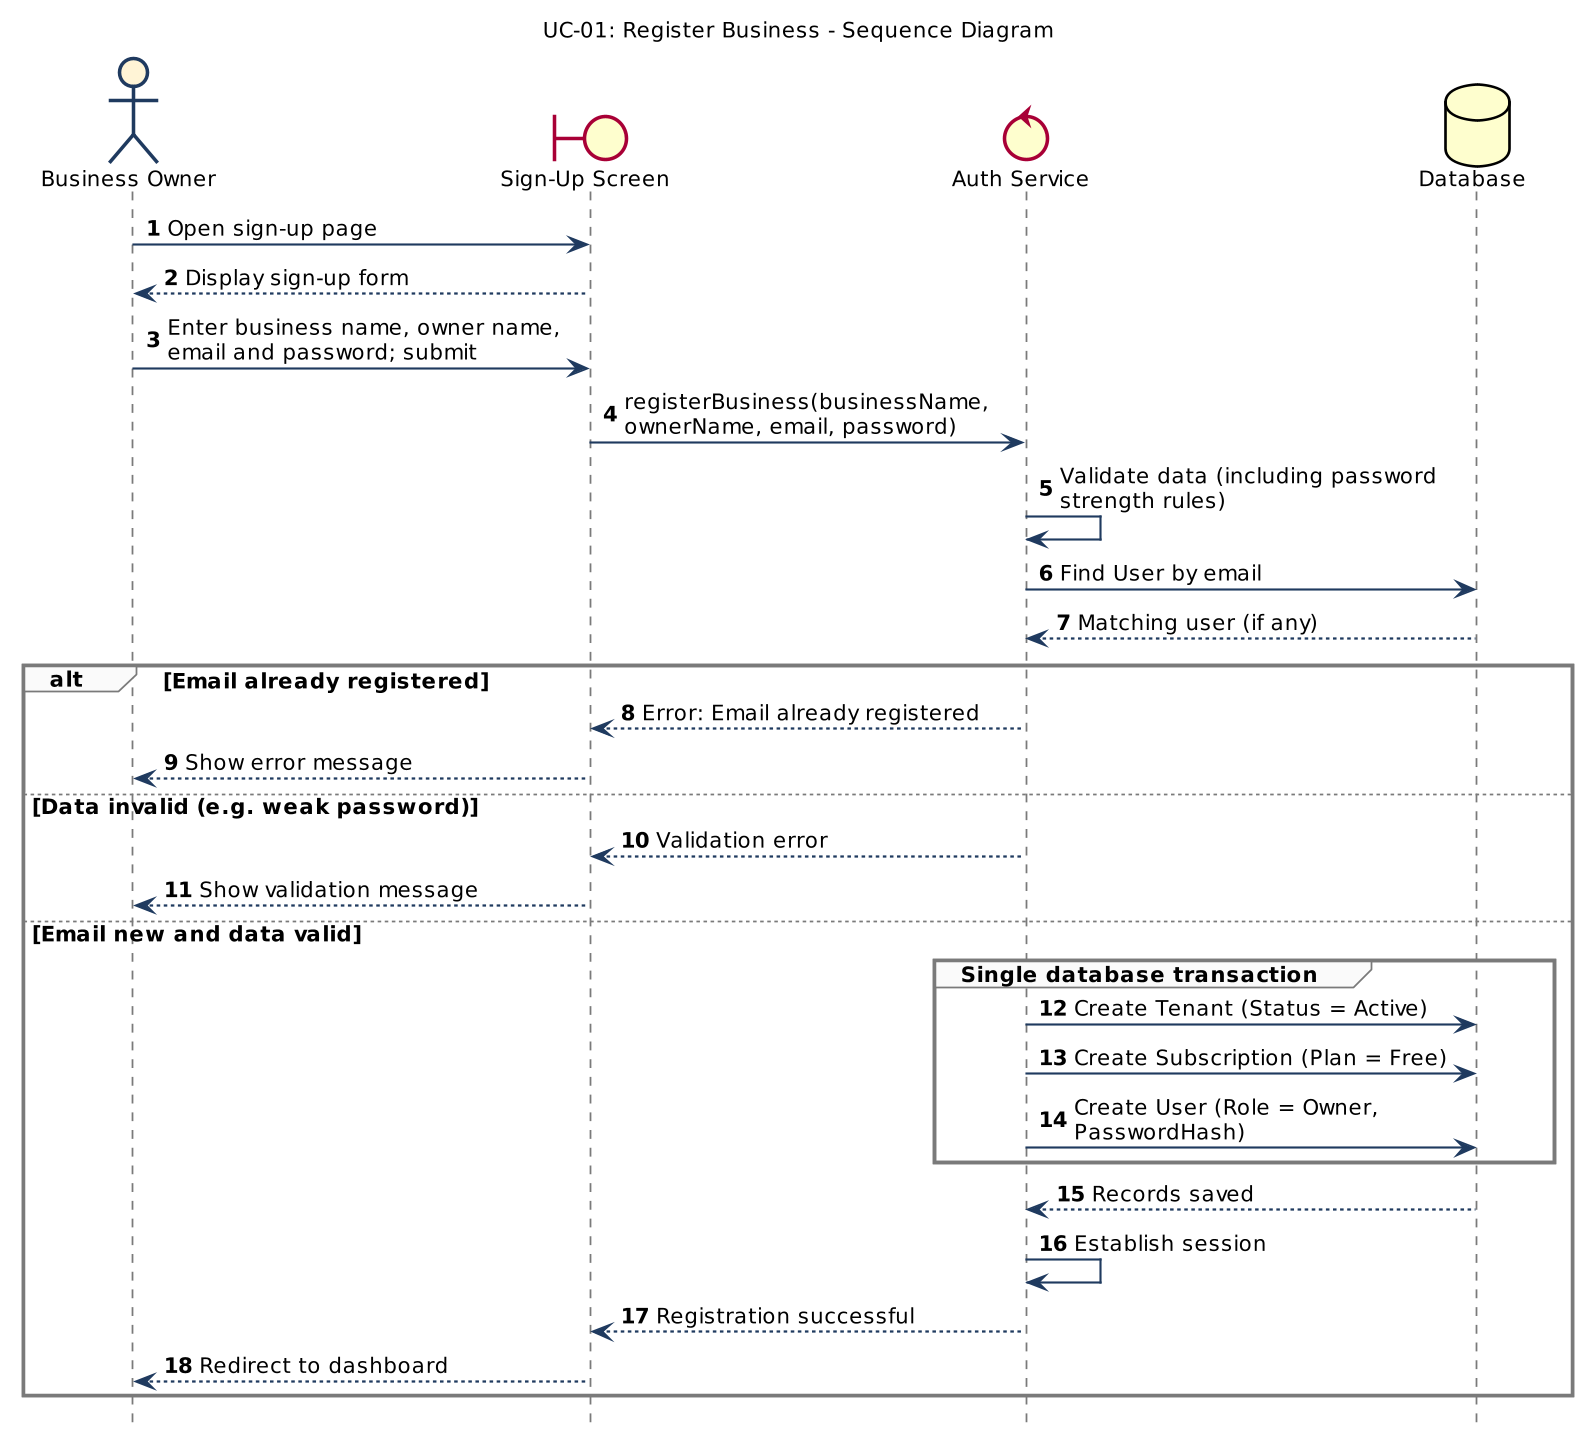
\includegraphics[width=\textwidth,height=0.85\textheight,keepaspectratio]{Figures/SequenceDiagrams/UC01_Register_Business.png}
    \caption[Sequence Diagram: Register Business]{Sequence Diagram: Register Business\\ This figure shows the sequence diagram of UC-01 (Register Business)}
    \label{fig:seq-uc1}
\end{figure}

\subsection{UC-02: Login}
 
This diagram shows the interaction for the use case \textbf{Login} (UC-02).
 
\begin{figure}[H]
    \centering
    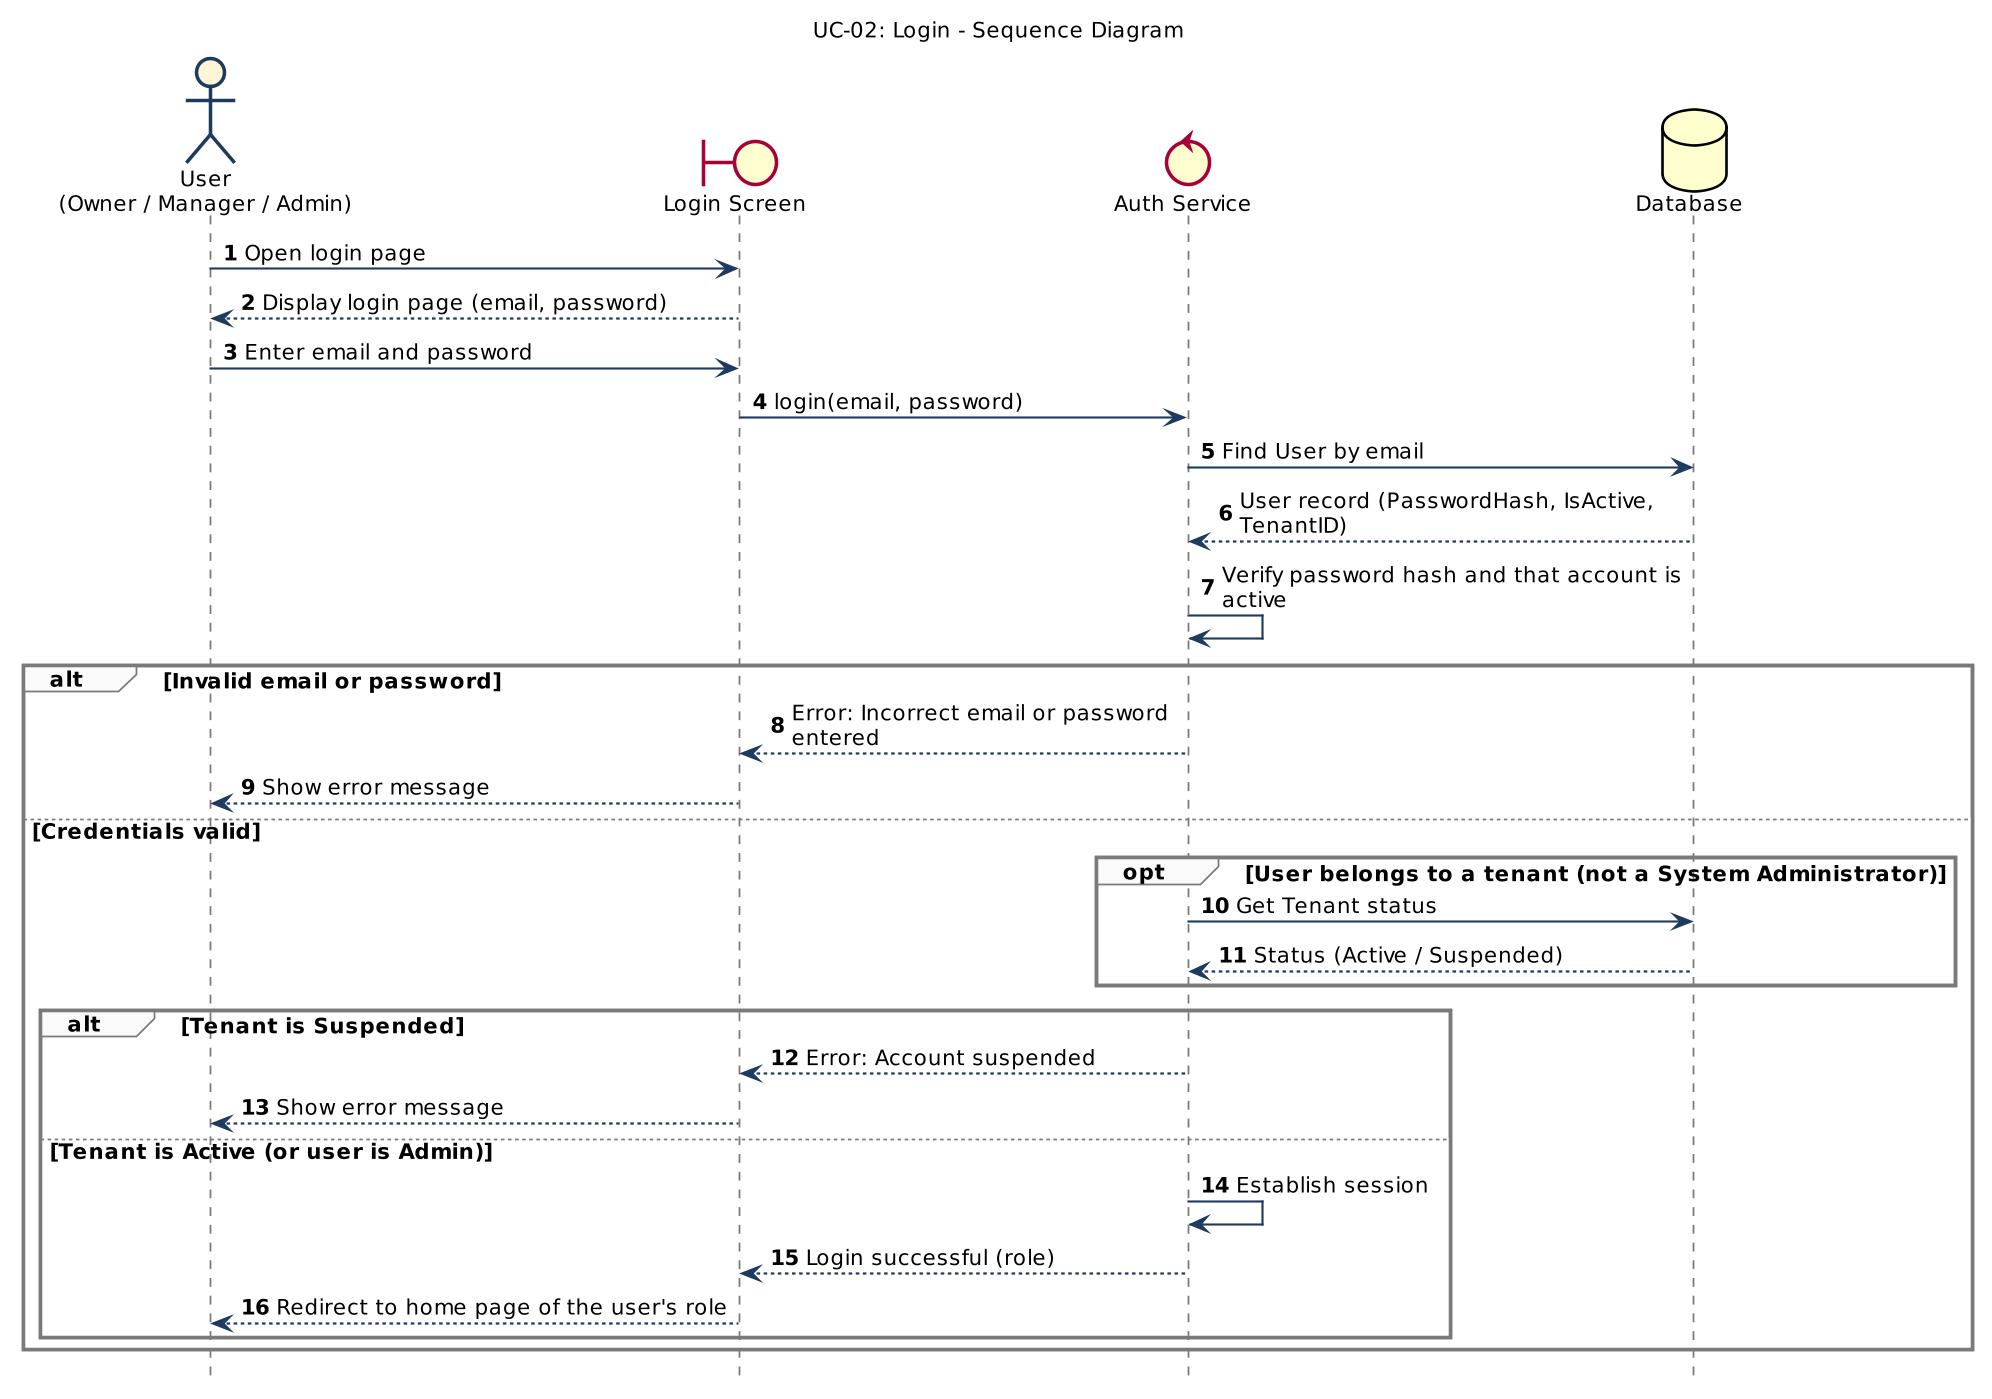
\includegraphics[width=\textwidth,height=0.85\textheight,keepaspectratio]{Figures/SequenceDiagrams/UC02_Login.png}
    \caption[Sequence Diagram: Login]{Sequence Diagram: Login\\ This figure shows the sequence diagram of UC-02 (Login)}
    \label{fig:seq-uc2}
\end{figure}
 
\subsection{UC-03: Manage Stores}
 
This diagram shows the interaction for the use case \textbf{Manage Stores} (UC-03).
 
\begin{figure}[H]
    \centering
    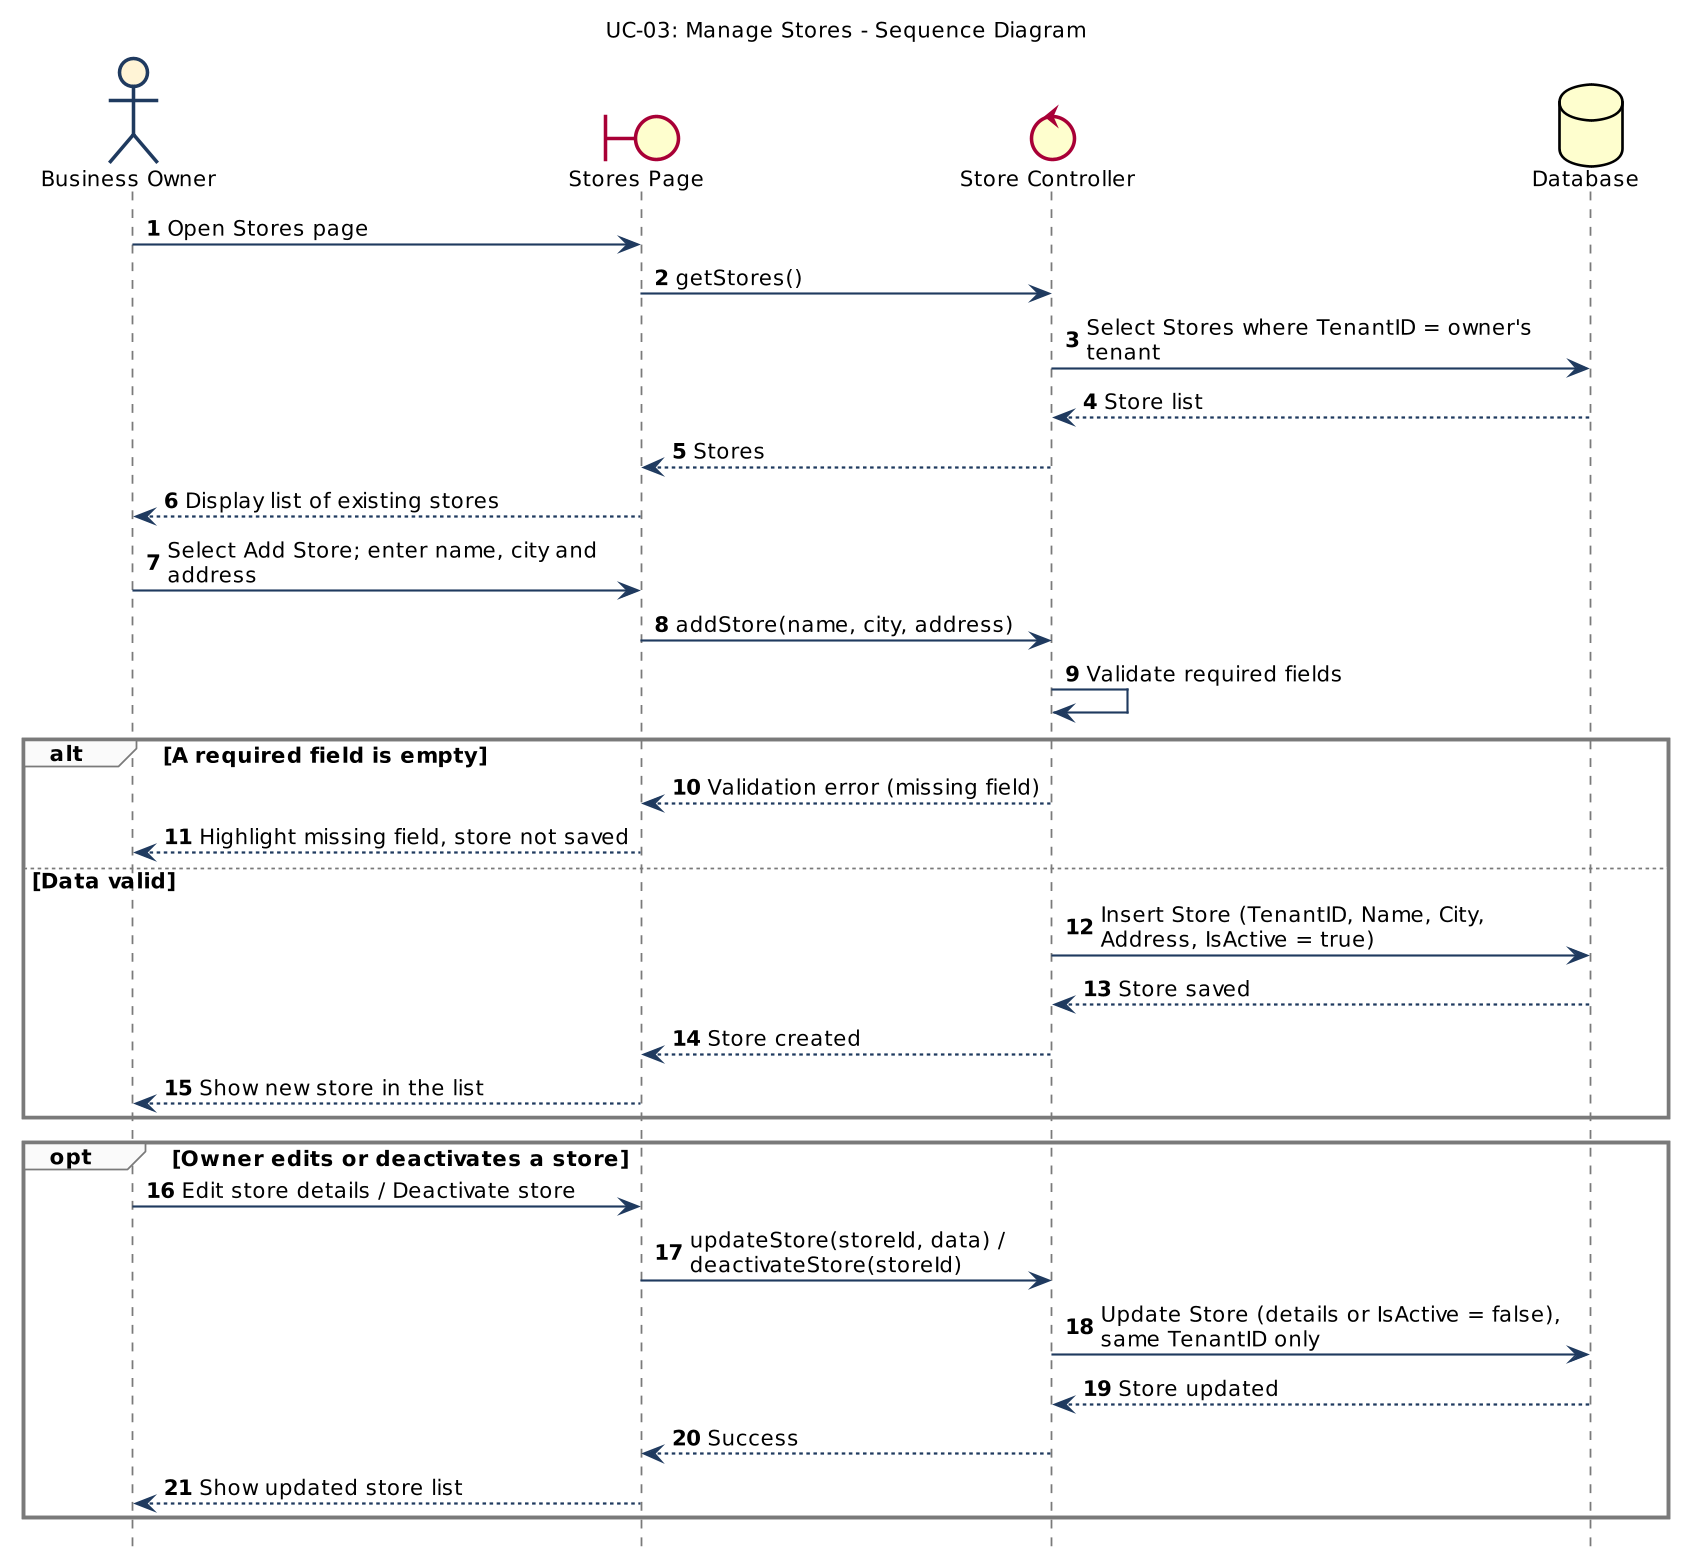
\includegraphics[width=\textwidth,height=0.85\textheight,keepaspectratio]{Figures/SequenceDiagrams/UC03_Manage_Stores.png}
    \caption[Sequence Diagram: Manage Stores]{Sequence Diagram: Manage Stores\\ This figure shows the sequence diagram of UC-03 (Manage Stores)}
    \label{fig:seq-uc3}
\end{figure}

\subsection{UC-04: Manage Store Managers}
 
This diagram shows the interaction for the use case \textbf{Manage Store Managers} (UC-04).
 
\begin{figure}[H]
    \centering
    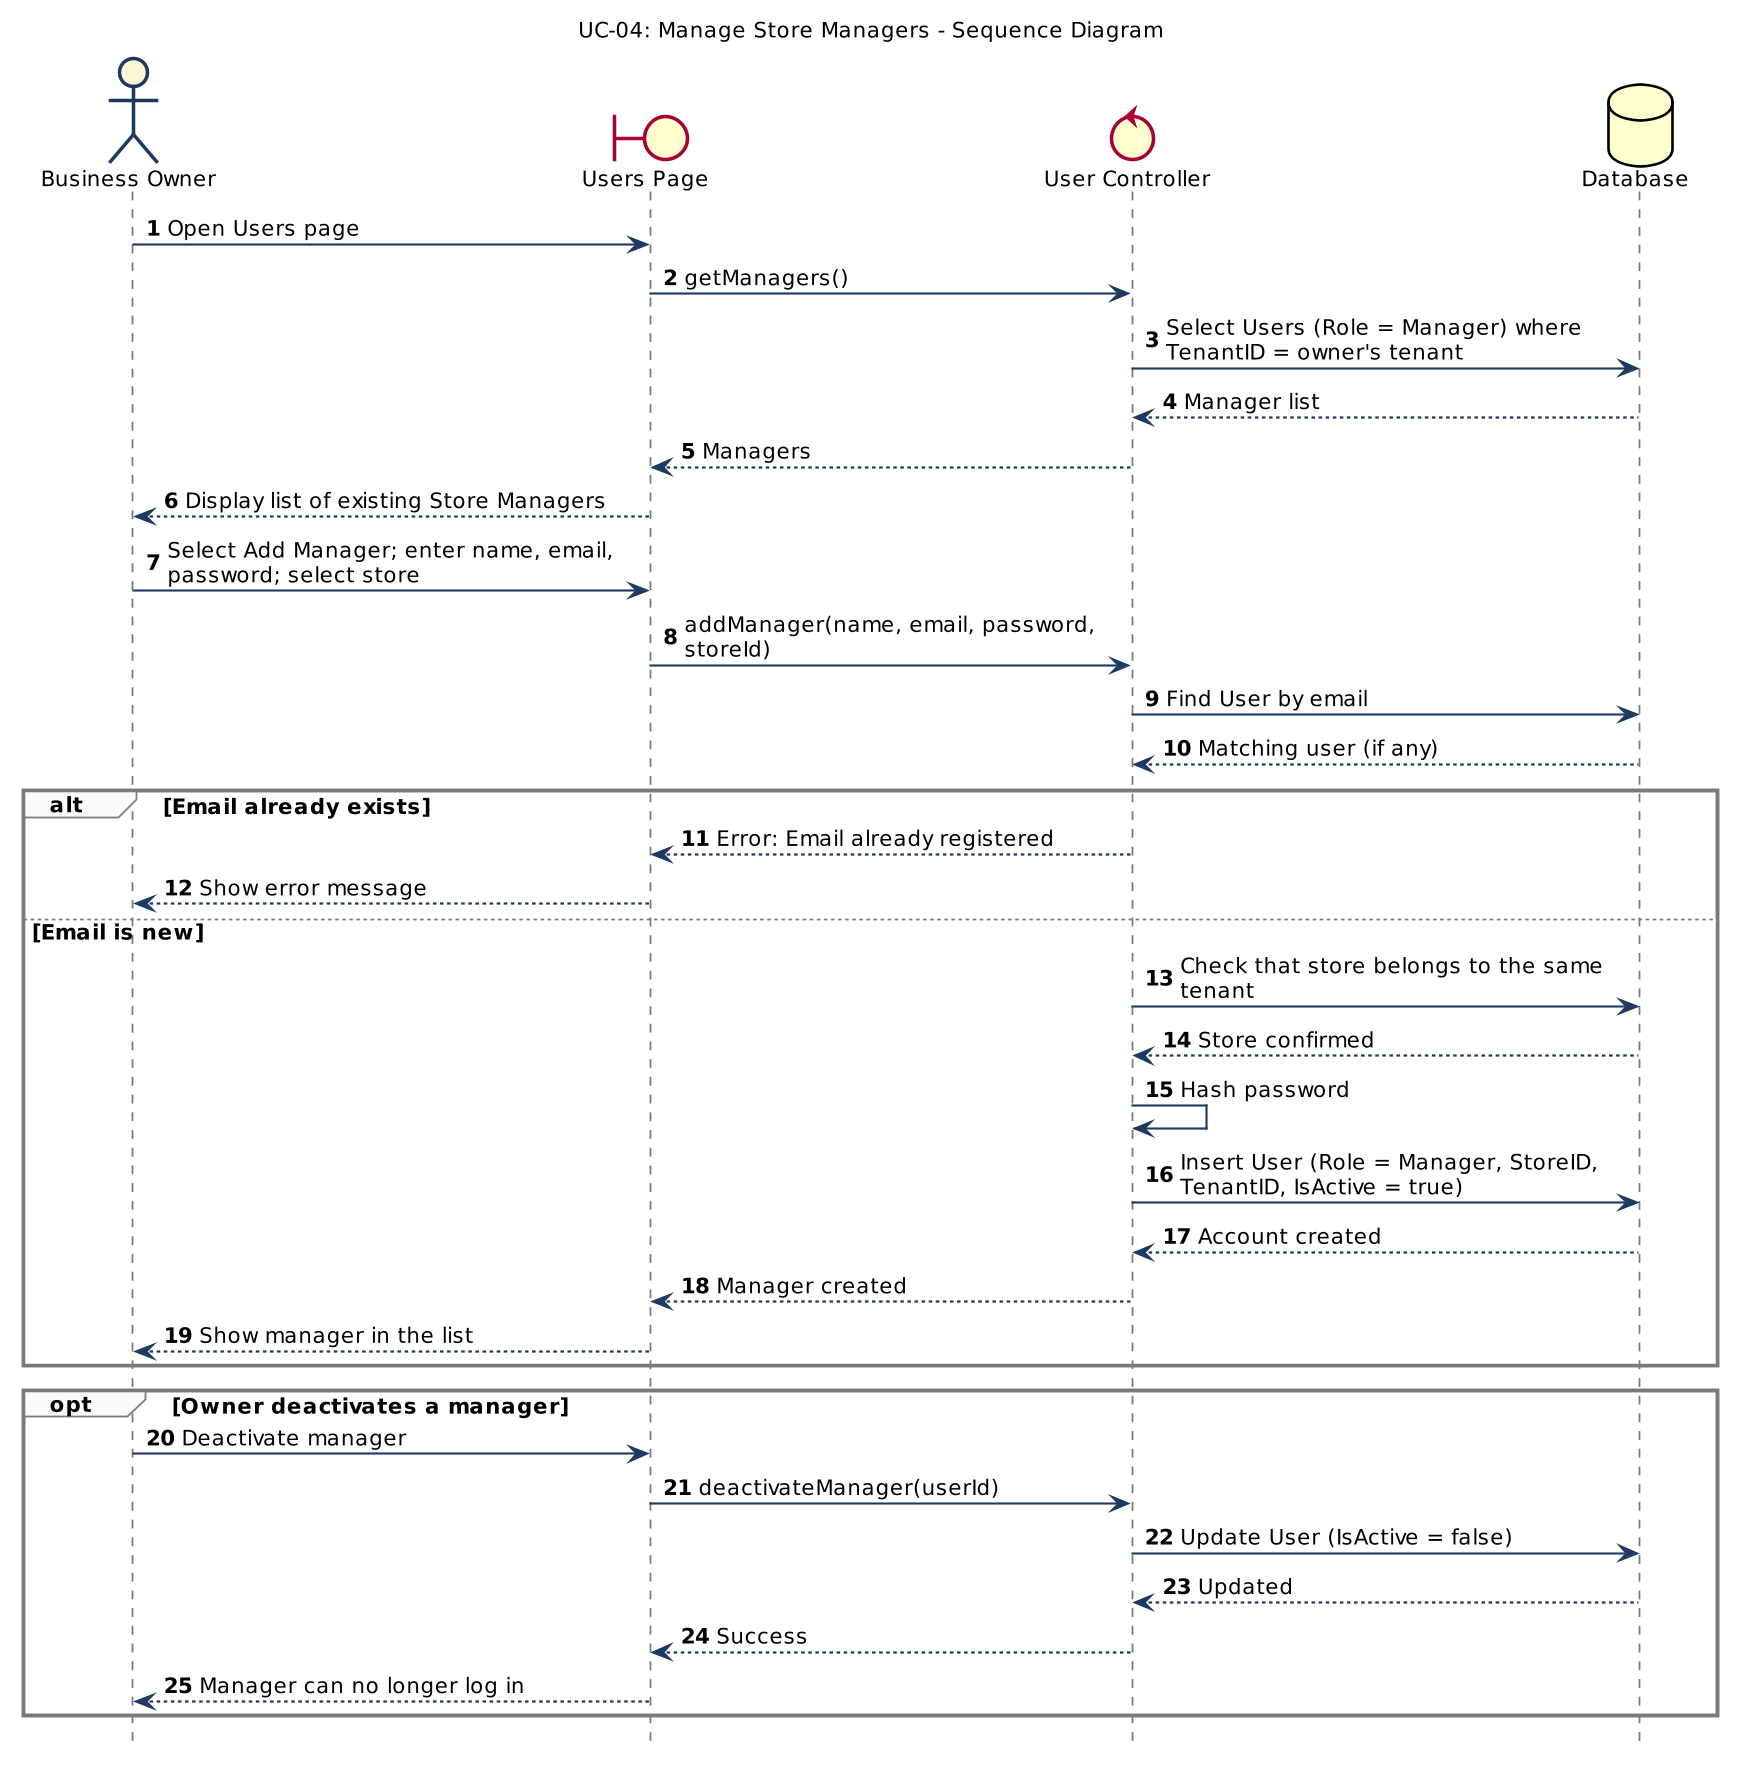
\includegraphics[width=\textwidth,height=0.85\textheight,keepaspectratio]{Figures/SequenceDiagrams/UC04_Manage_Store_Managers.png}
    \caption[Sequence Diagram: Manage Store Managers]{Sequence Diagram: Manage Store Managers\\ This figure shows the sequence diagram of UC-04 (Manage Store Managers)}
    \label{fig:seq-uc4}
\end{figure}
 
\subsection{UC-05: Manage Products and Variants}
 
This diagram shows the interaction for the use case \textbf{Manage Products and Variants} (UC-05).
 
\begin{figure}[H]
    \centering
    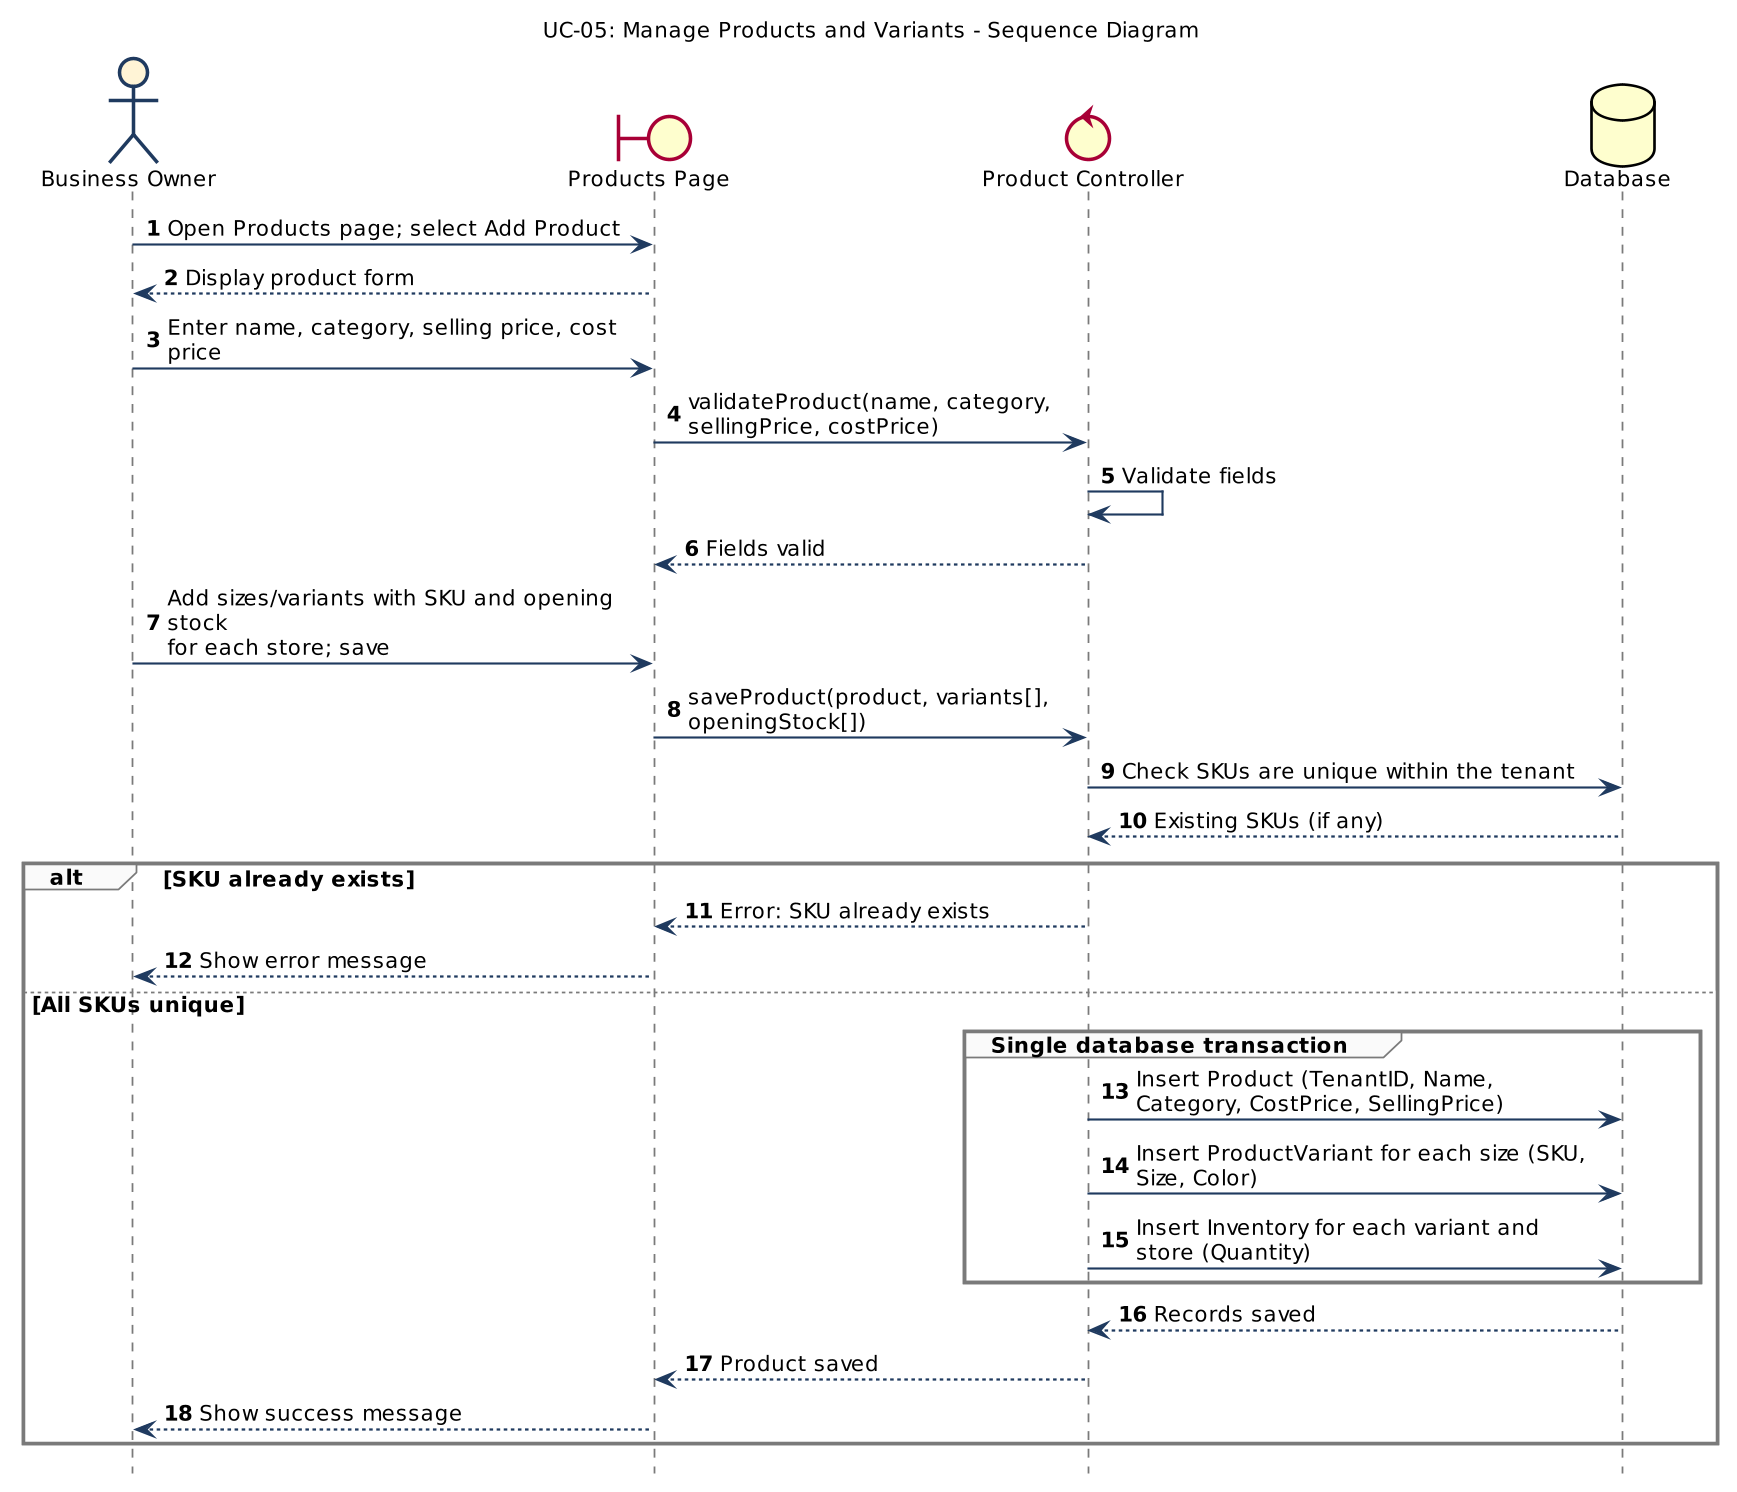
\includegraphics[width=\textwidth,height=0.85\textheight,keepaspectratio]{Figures/SequenceDiagrams/UC05_Manage_Products_and_Variants.png}
    \caption[Sequence Diagram: Manage Products and Variants]{Sequence Diagram: Manage Products and Variants\\ This figure shows the sequence diagram of UC-05 (Manage Products and Variants)}
    \label{fig:seq-uc5}
\end{figure}
 
\subsection{UC-06: Adjust Inventory}
 
This diagram shows the interaction for the use case \textbf{Adjust Inventory} (UC-06).
 
\begin{figure}[H]
    \centering
    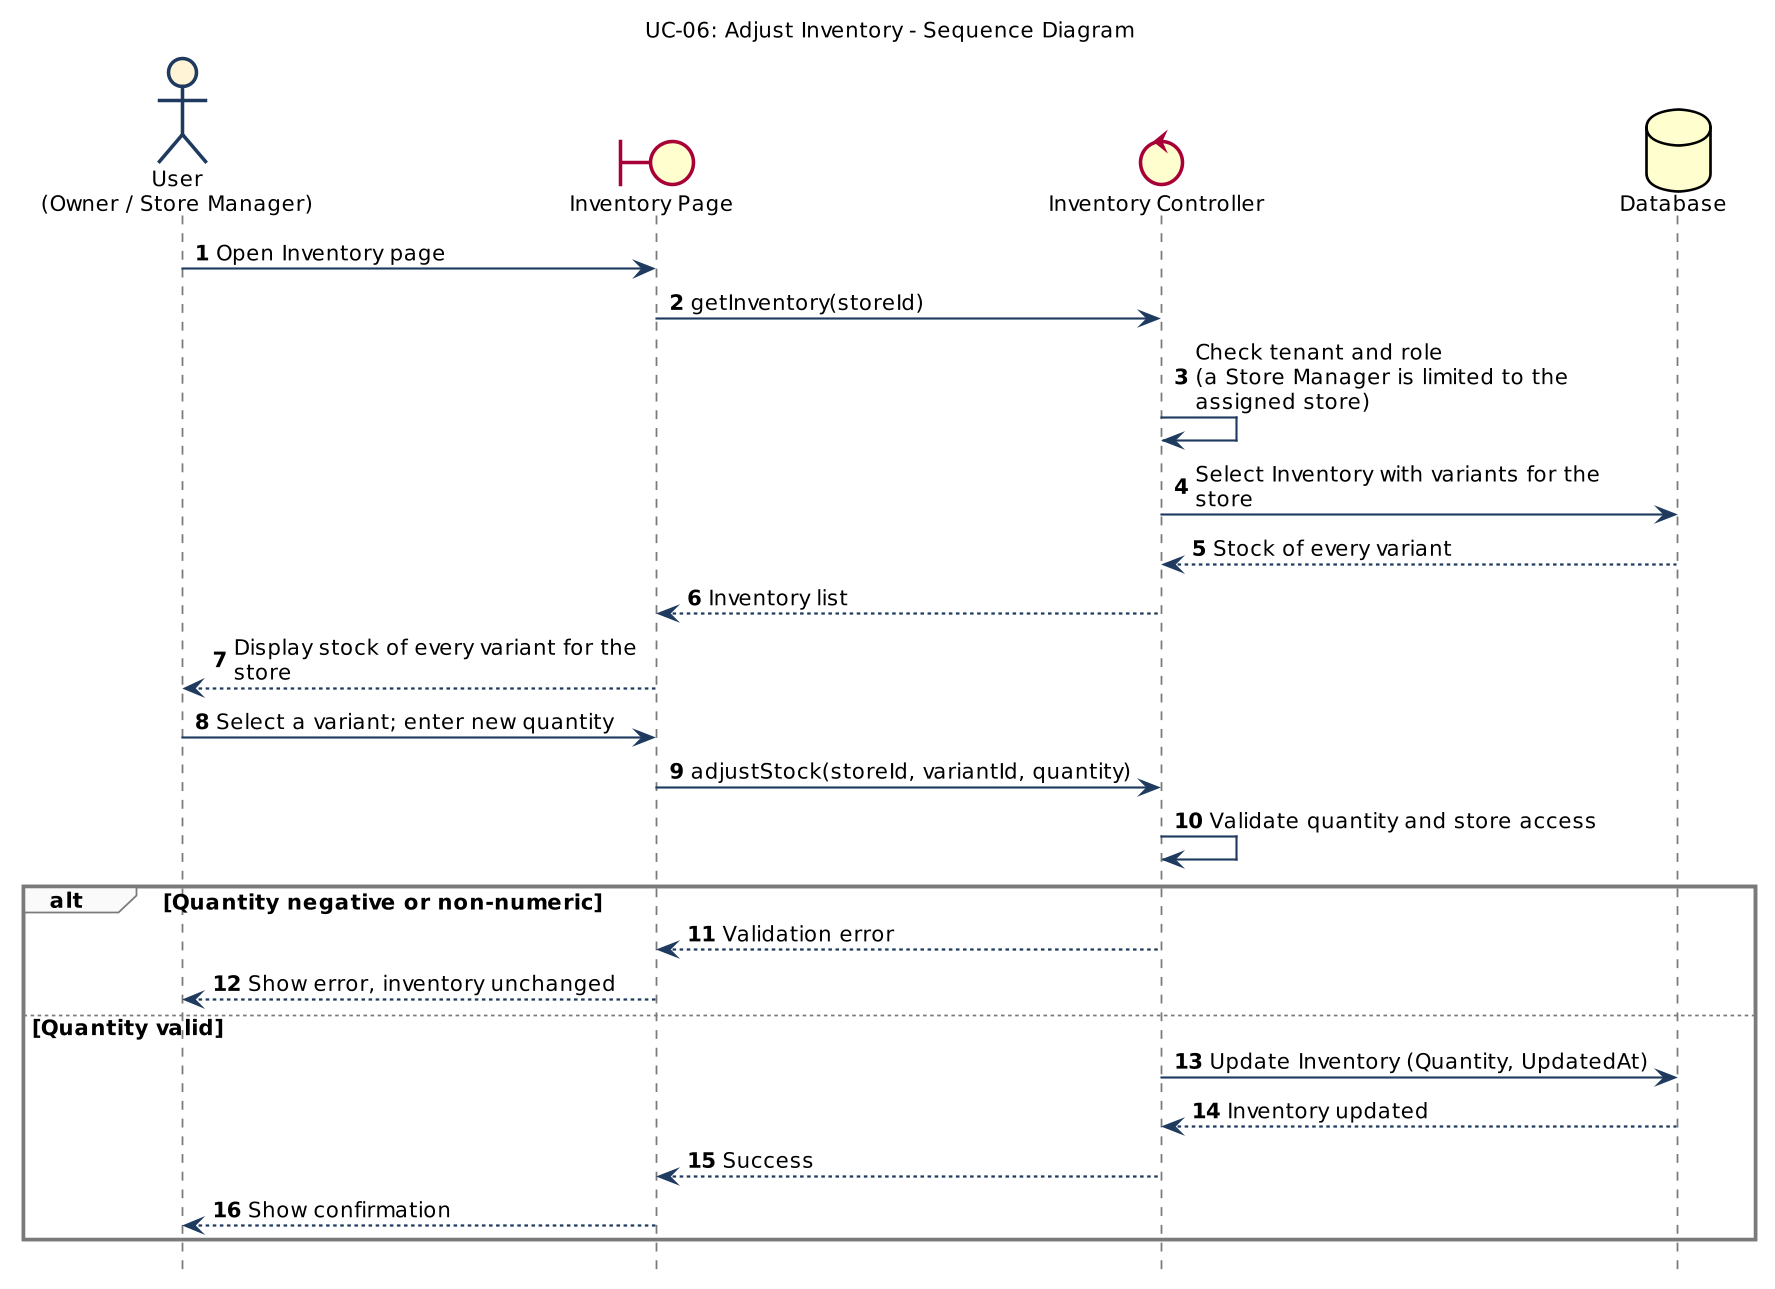
\includegraphics[width=\textwidth,height=0.85\textheight,keepaspectratio]{Figures/SequenceDiagrams/UC06_Adjust_Inventory.png}
    \caption[Sequence Diagram: Adjust Inventory]{Sequence Diagram: Adjust Inventory\\ This figure shows the sequence diagram of UC-06 (Adjust Inventory)}
    \label{fig:seq-uc6}
\end{figure}
 
\subsection{UC-07: Record Sale (POS)}
 
This diagram shows the interaction for the use case \textbf{Record Sale (POS)} (UC-07).
 
\begin{figure}[H]
    \centering
    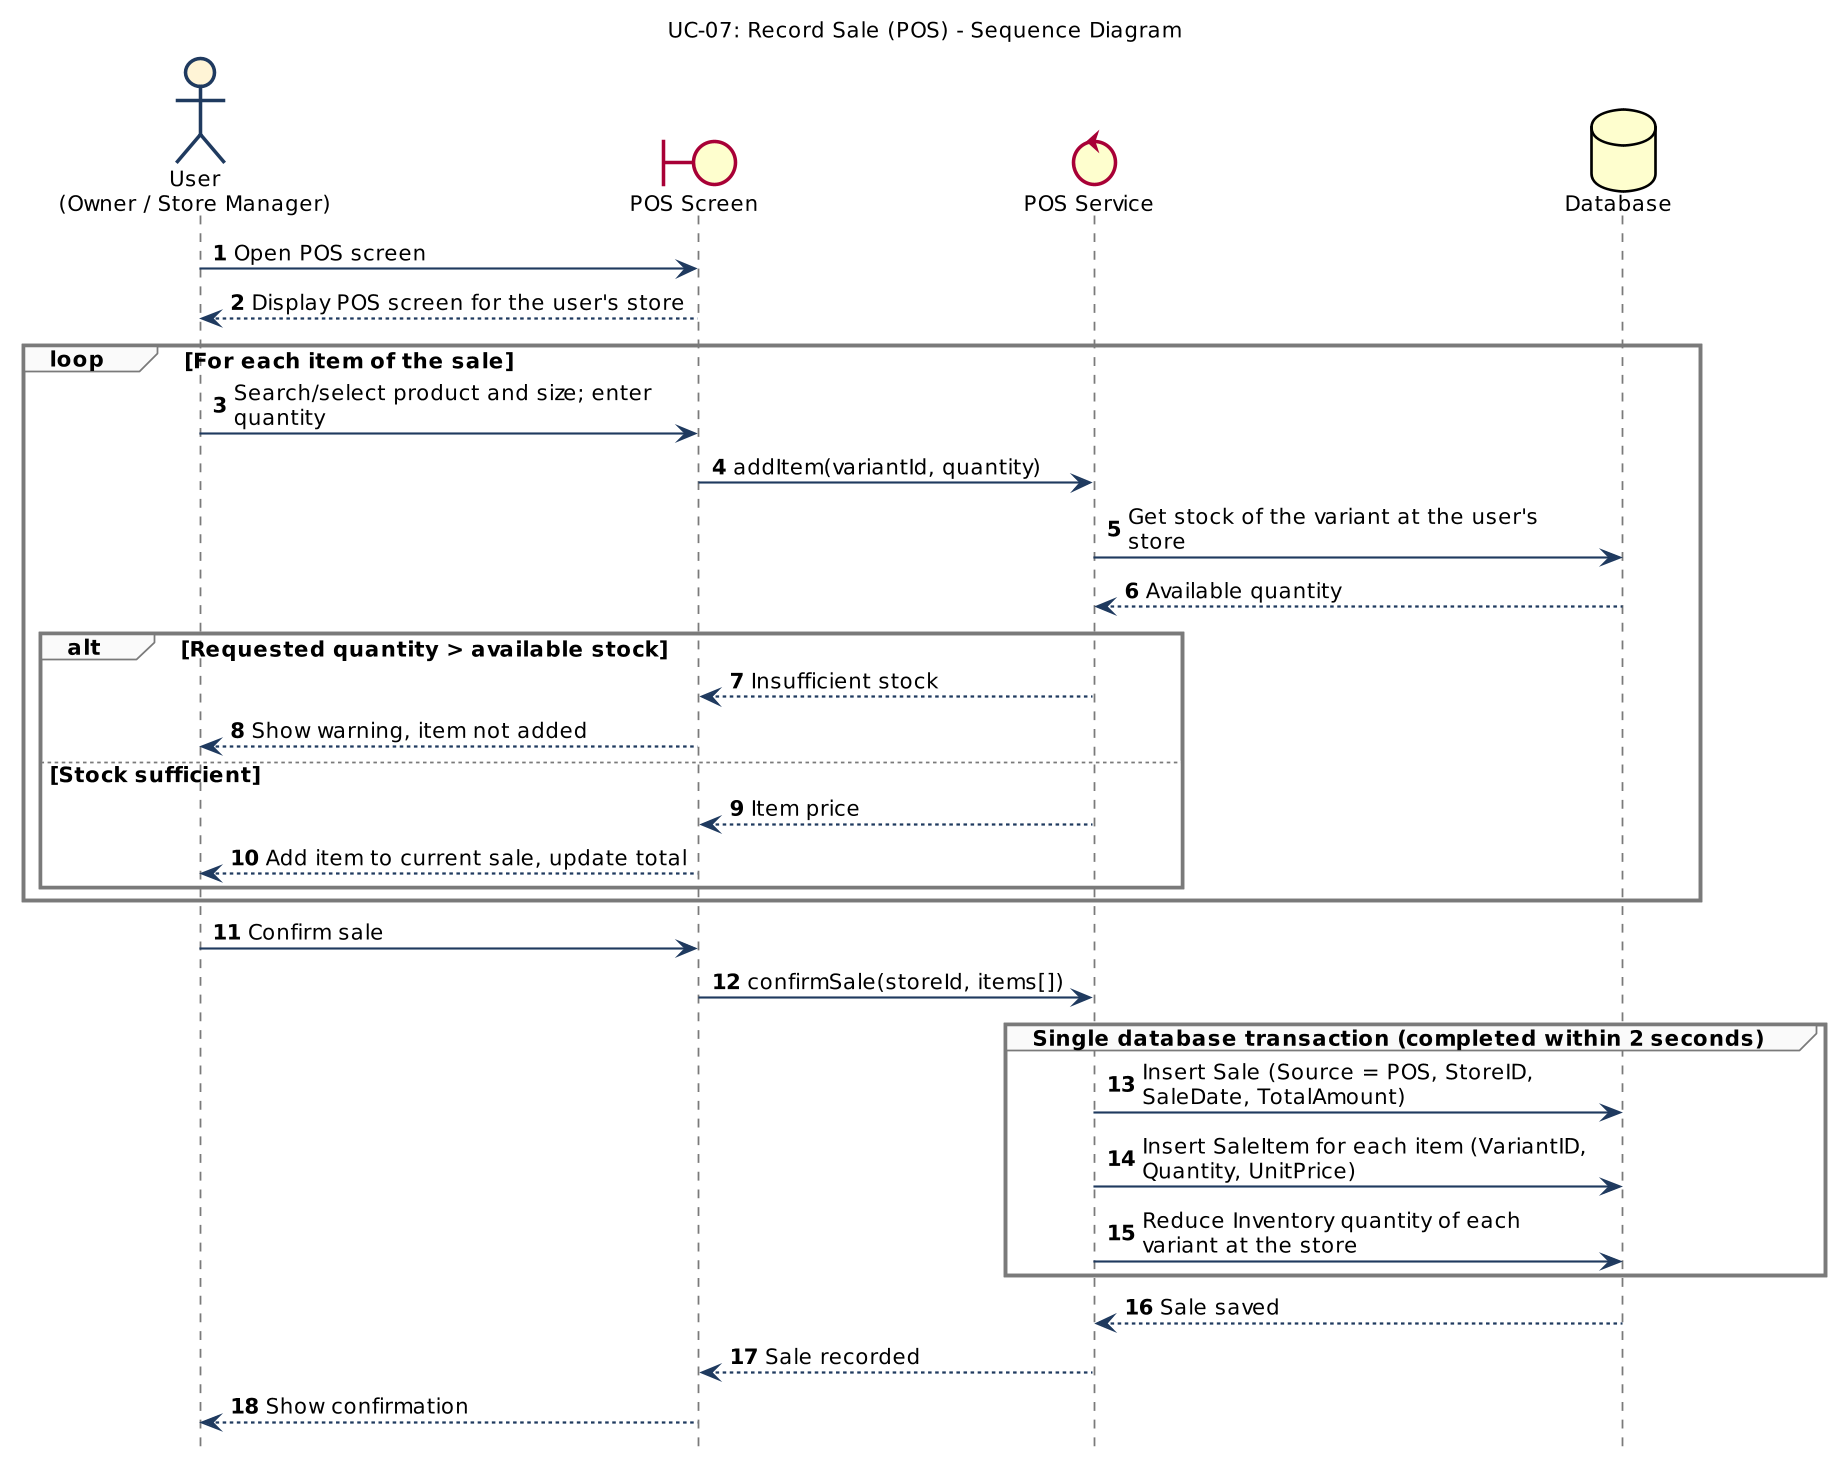
\includegraphics[width=\textwidth,height=0.85\textheight,keepaspectratio]{Figures/SequenceDiagrams/UC07_Record_Sale_POS.png}
    \caption[Sequence Diagram: Record Sale (POS)]{Sequence Diagram: Record Sale (POS)\\ This figure shows the sequence diagram of UC-07 (Record Sale (POS))}
    \label{fig:seq-uc7}
\end{figure}
 
\subsection{UC-08: Upload Historical Sales Data}
 
This diagram shows the interaction for the use case \textbf{Upload Historical Sales Data} (UC-08).
 
\begin{figure}[H]
    \centering
    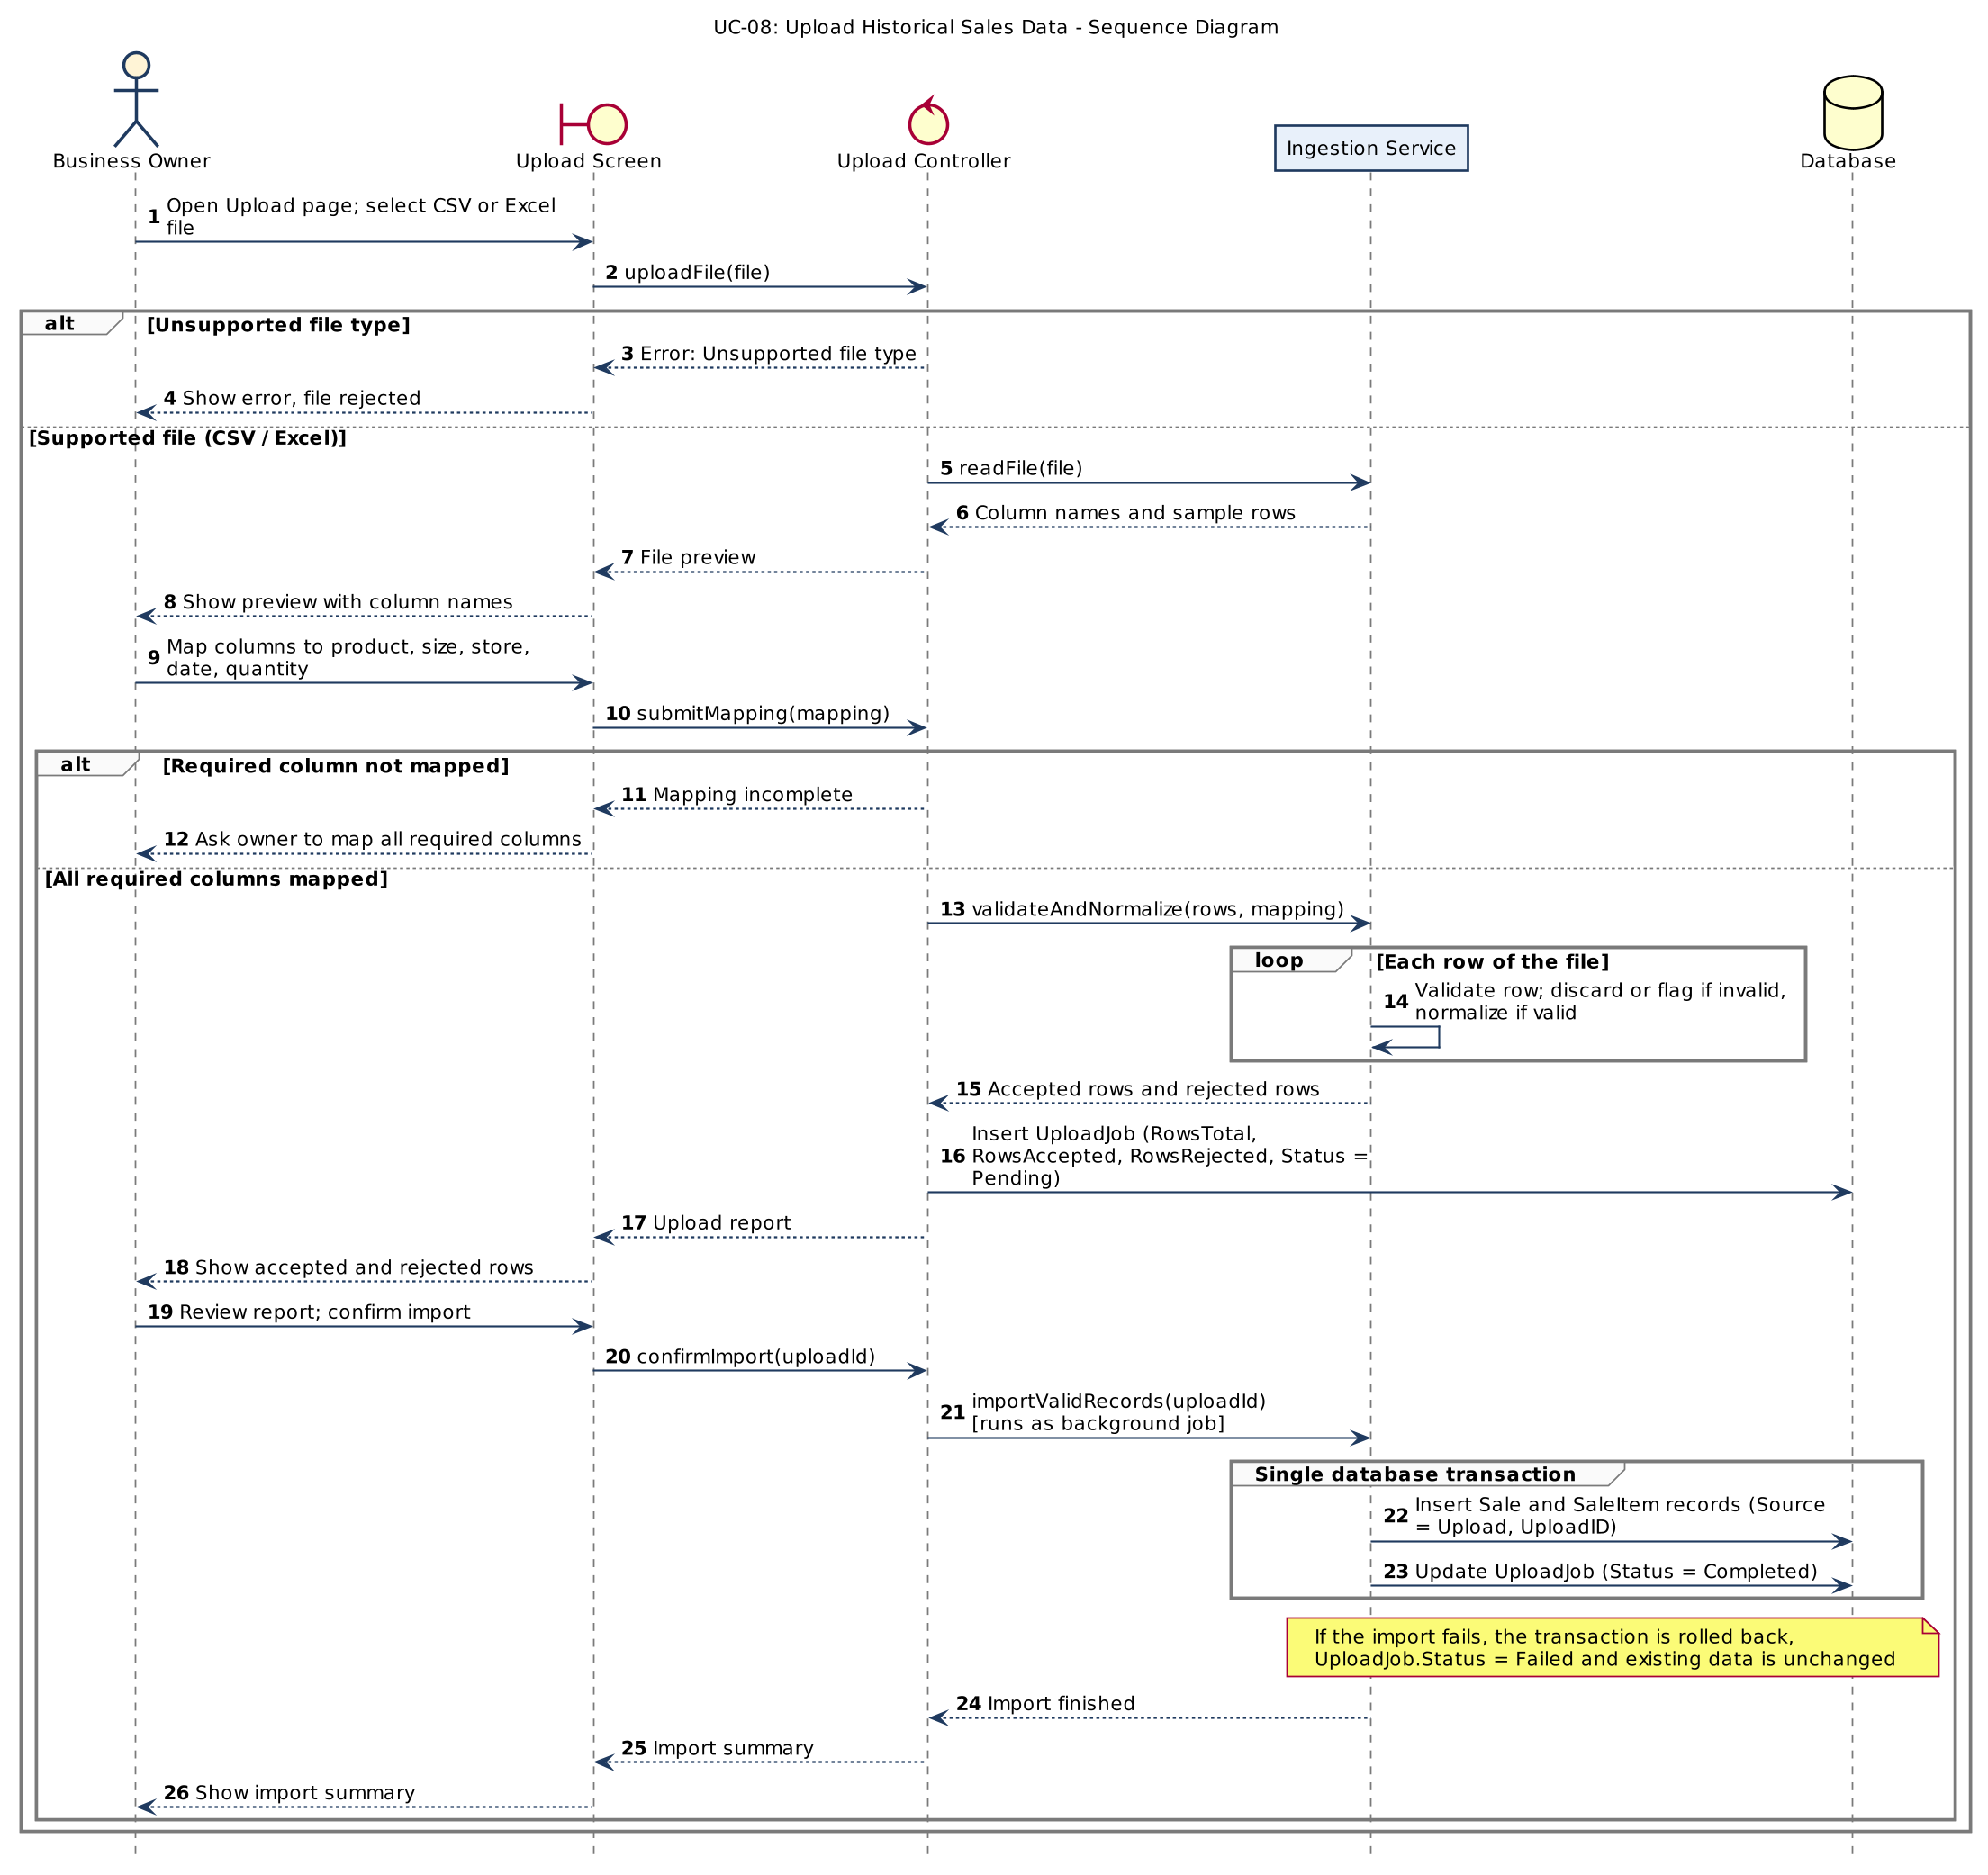
\includegraphics[width=\textwidth,height=0.85\textheight,keepaspectratio]{Figures/SequenceDiagrams/UC08_Upload_Historical_Sales_Data.png}
    \caption[Sequence Diagram: Upload Historical Sales Data]{Sequence Diagram: Upload Historical Sales Data\\ This figure shows the sequence diagram of UC-08 (Upload Historical Sales Data)}
    \label{fig:seq-uc8}
\end{figure}
 
\subsection{UC-09: View Dashboard and Alerts}
 
This diagram shows the interaction for the use case \textbf{View Dashboard and Alerts} (UC-09).
 
\begin{figure}[H]
    \centering
    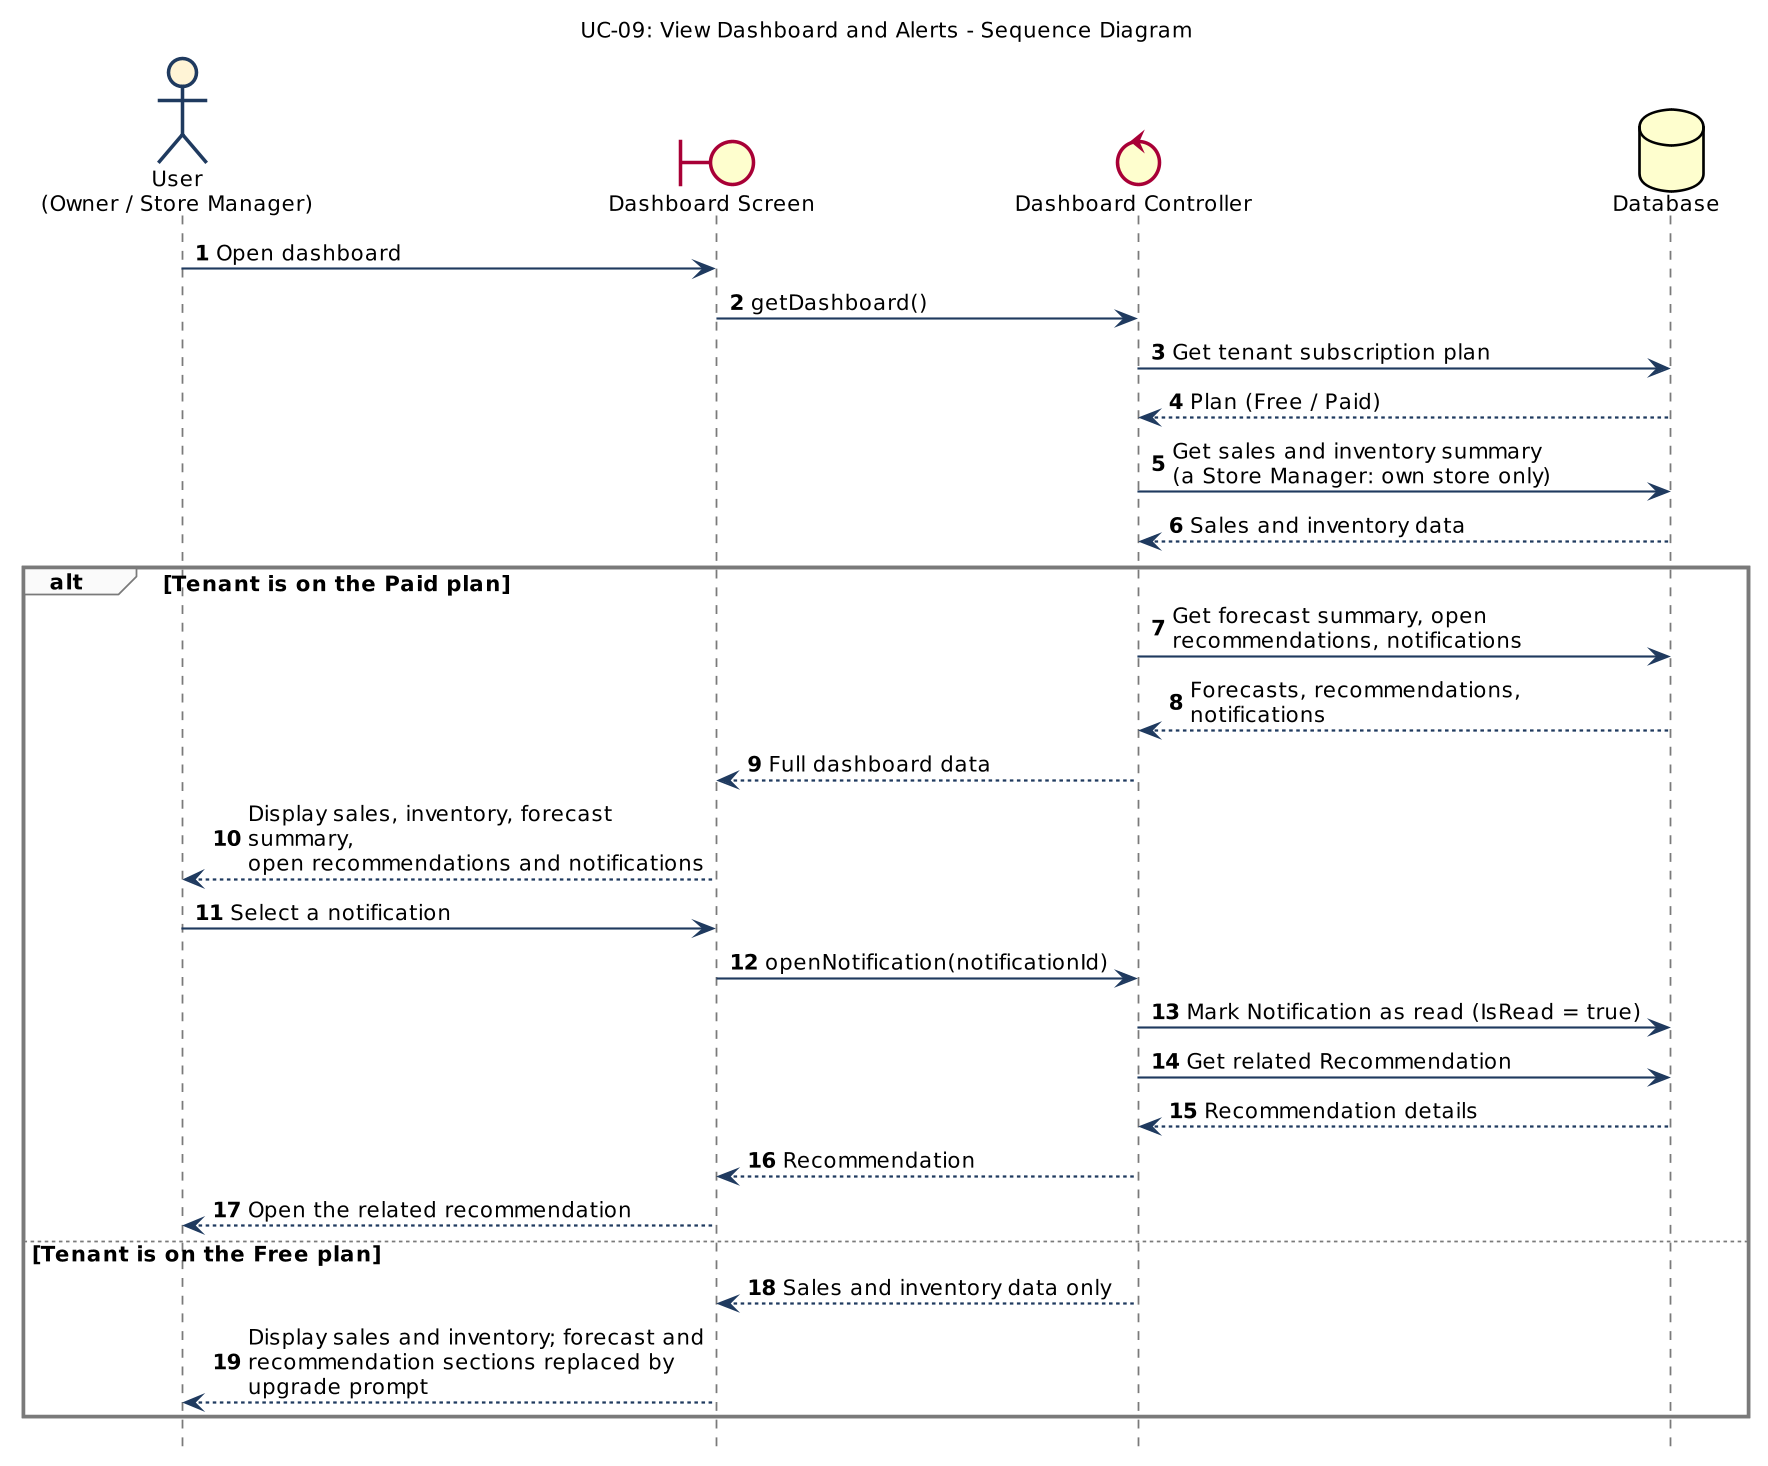
\includegraphics[width=\textwidth,height=0.85\textheight,keepaspectratio]{Figures/SequenceDiagrams/UC09_View_Dashboard_and_Alerts.png}
    \caption[Sequence Diagram: View Dashboard and Alerts]{Sequence Diagram: View Dashboard and Alerts\\ This figure shows the sequence diagram of UC-09 (View Dashboard and Alerts)}
    \label{fig:seq-uc9}
\end{figure}


\subsection{UC-10: View Demand Forecast}
 
This diagram shows the interaction for the use case \textbf{View Demand Forecast} (UC-10).
 
\begin{figure}[H]
    \centering
    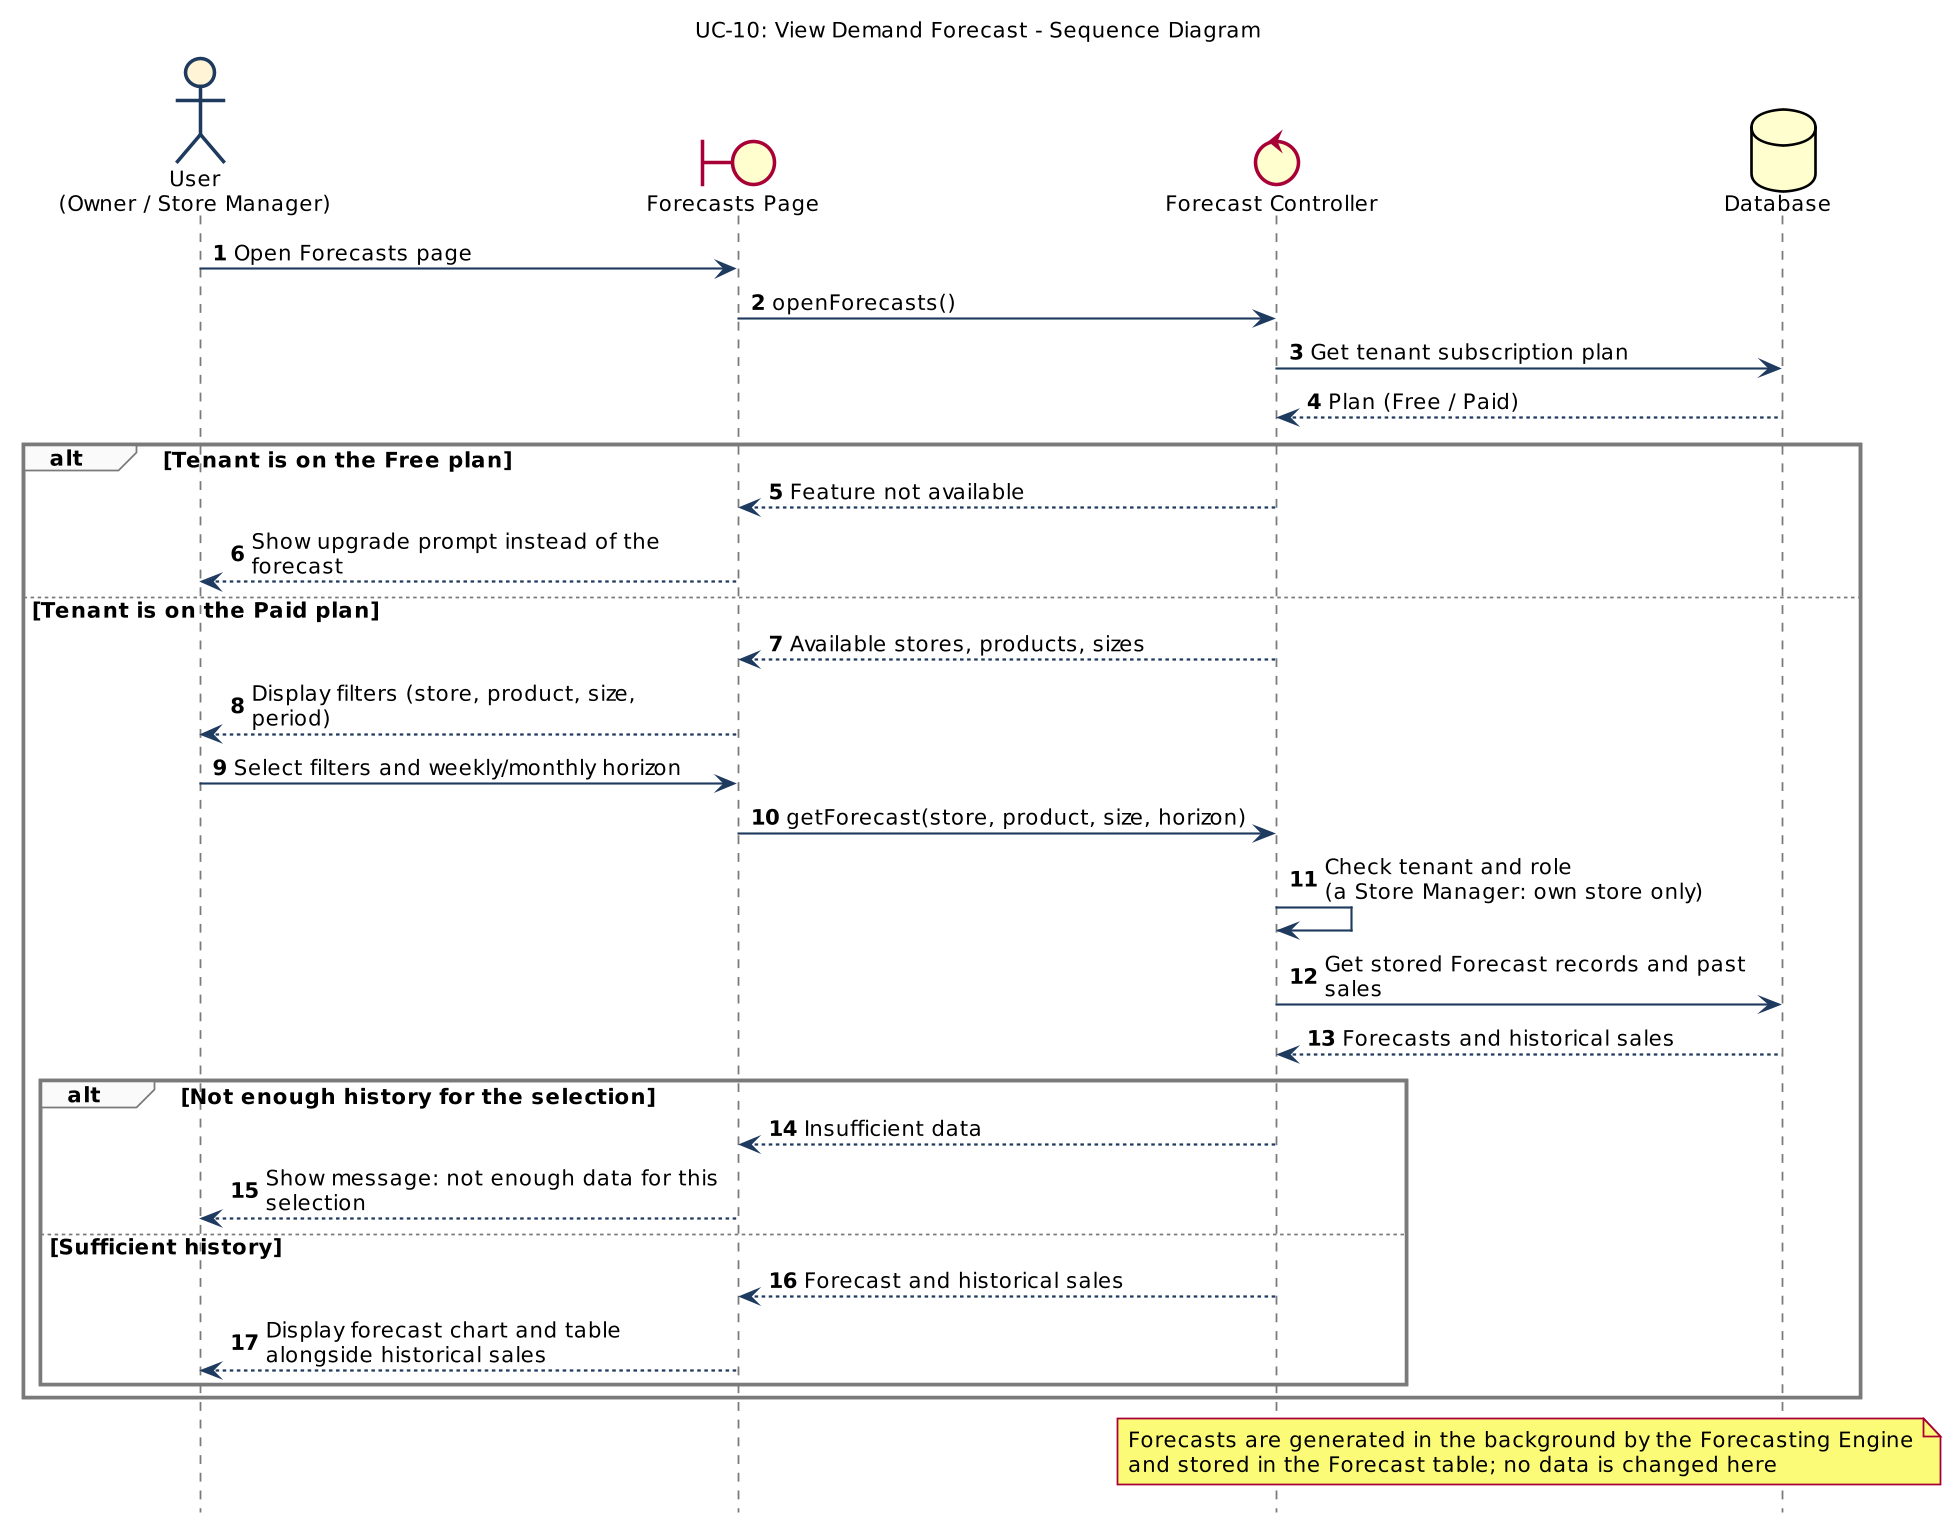
\includegraphics[width=\textwidth,height=0.85\textheight,keepaspectratio]{Figures/SequenceDiagrams/UC10_View_Demand_Forecast.png}
    \caption[Sequence Diagram: View Demand Forecast]{Sequence Diagram: View Demand Forecast\\ This figure shows the sequence diagram of UC-10 (View Demand Forecast)}
    \label{fig:seq-uc10}
\end{figure}
 
\subsection{UC-11: View and Act on Redistribution Recommendation}
 
This diagram shows the interaction for the use case \textbf{View and Act on Redistribution Recommendation} (UC-11).
 
\begin{figure}[H]
    \centering
    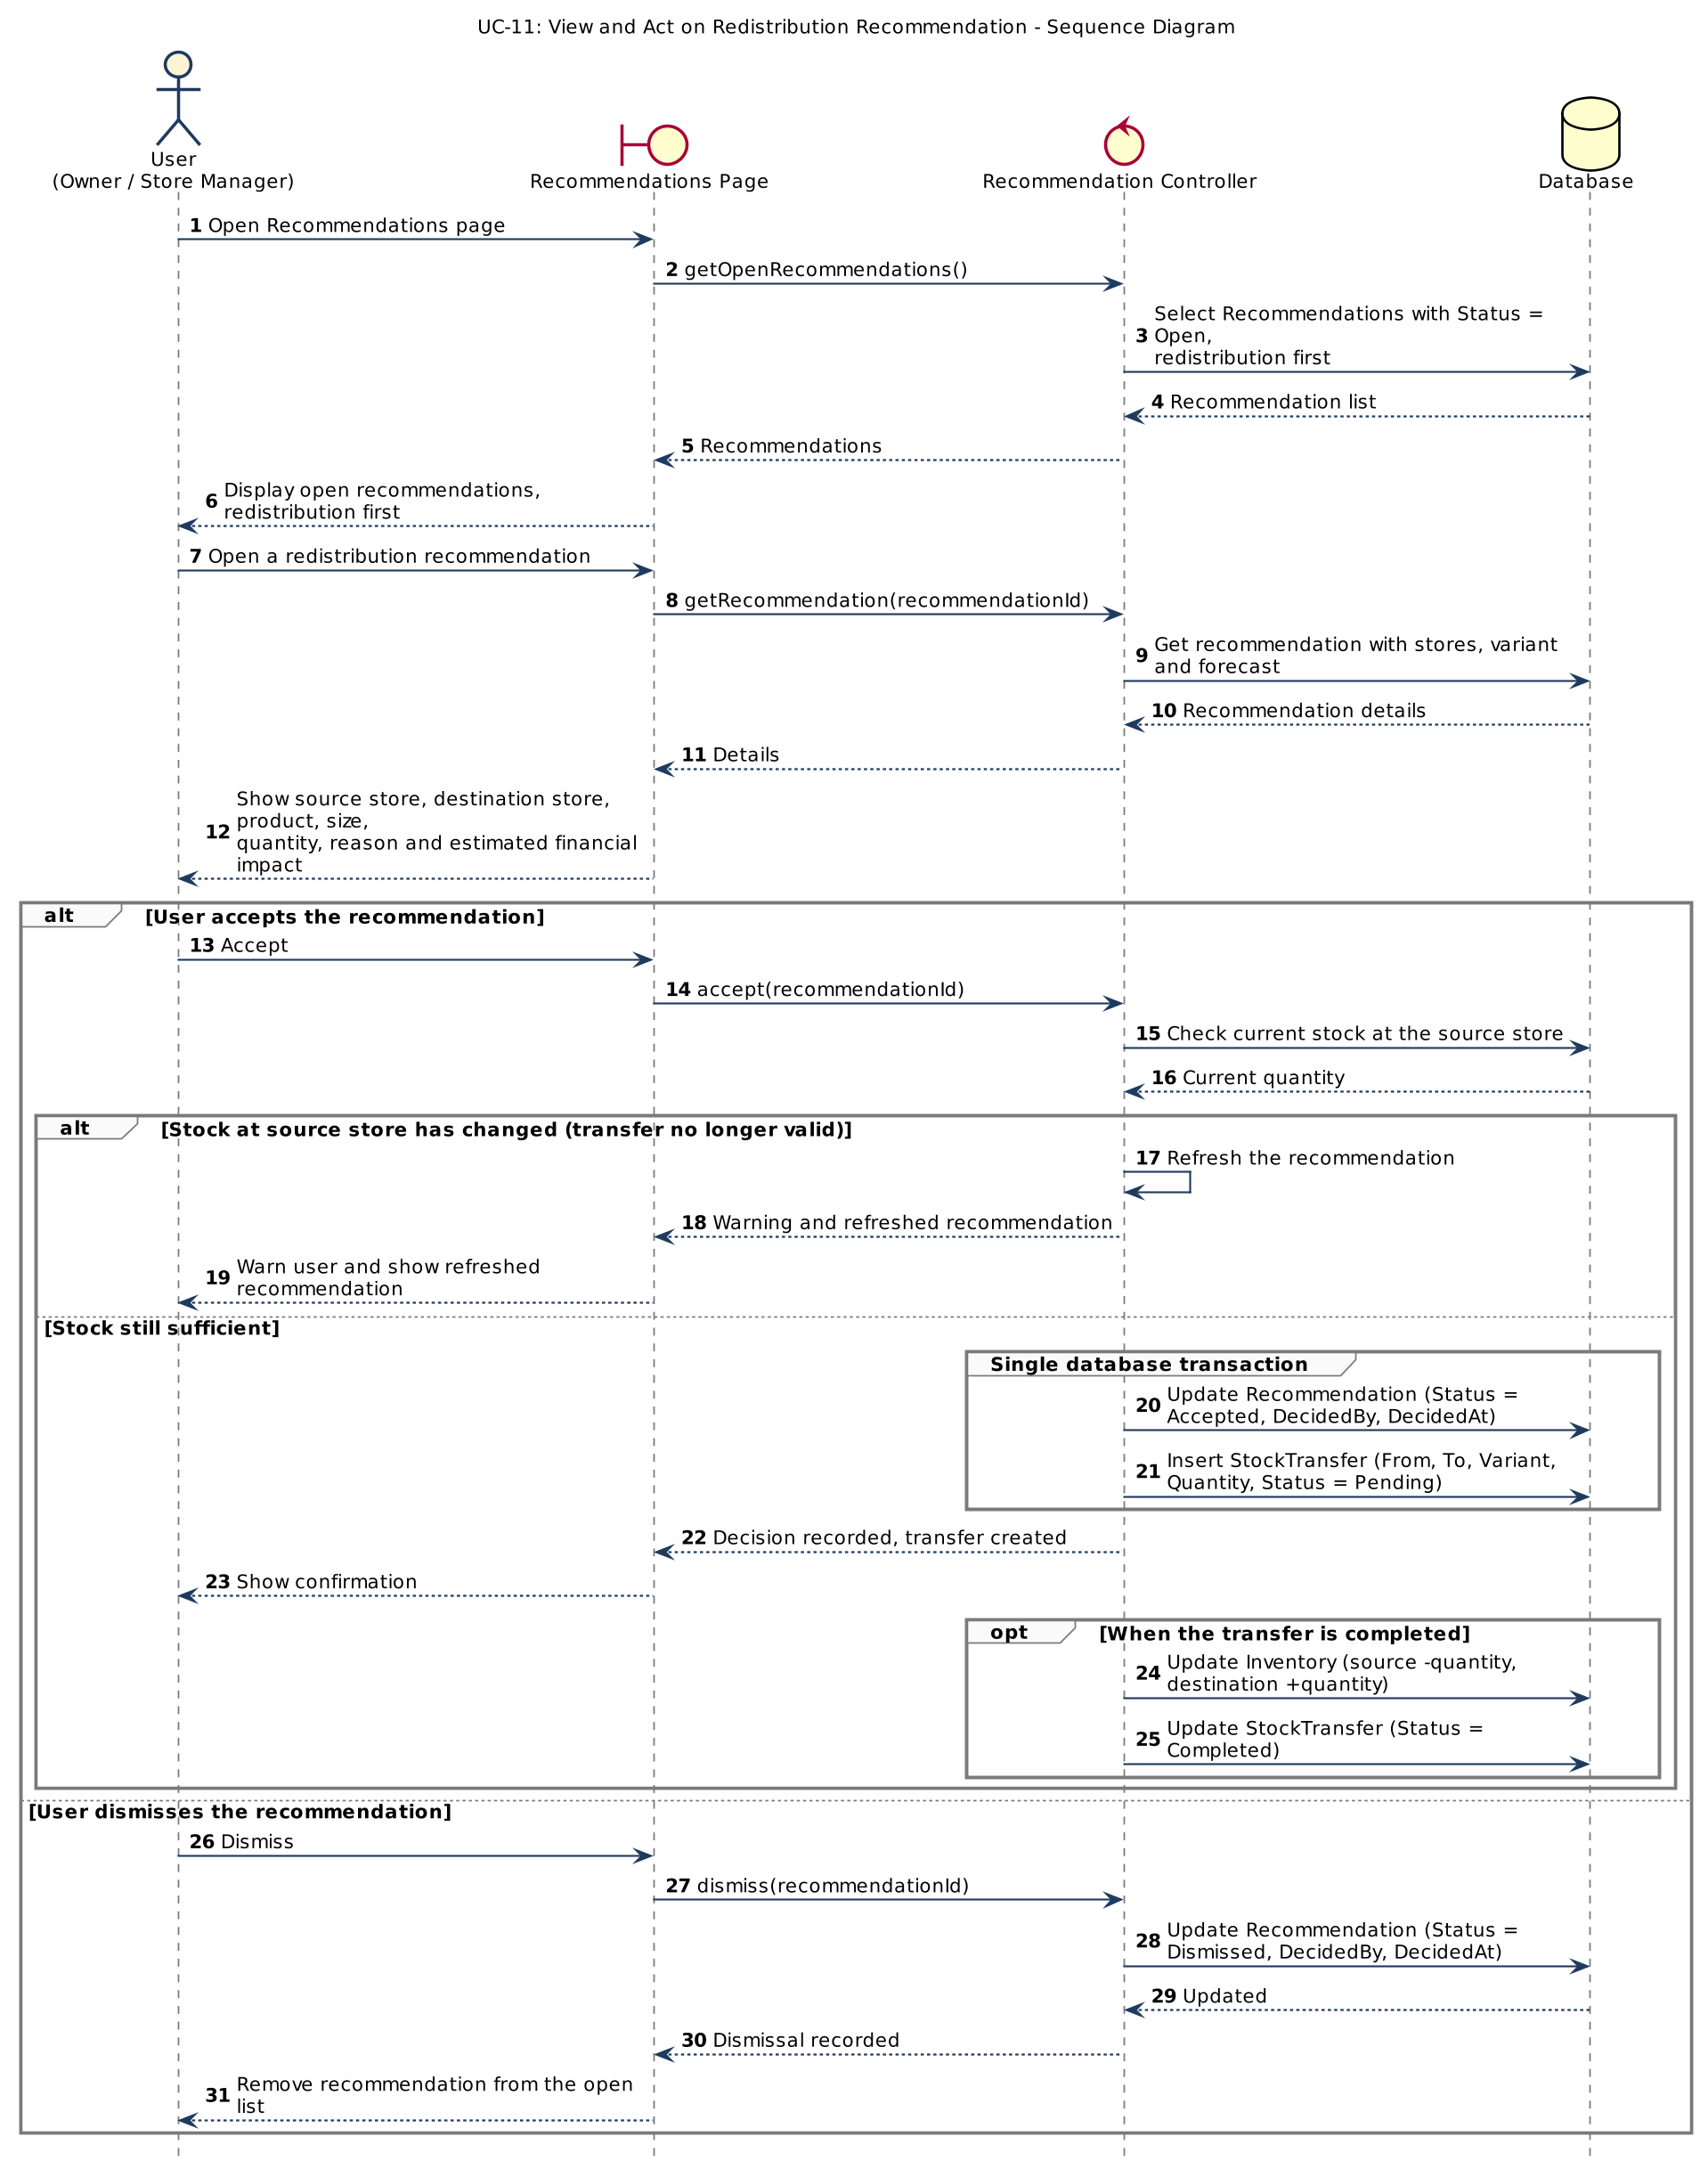
\includegraphics[width=\textwidth,height=0.85\textheight,keepaspectratio]{Figures/SequenceDiagrams/UC11_Redistribution_Recommendation.png}
    \caption[Sequence Diagram: View and Act on Redistribution Recommendation]{Sequence Diagram: View and Act on Redistribution Recommendation\\ This figure shows the sequence diagram of UC-11 (View and Act on Redistribution Recommendation)}
    \label{fig:seq-uc11}
\end{figure}
 
\subsection{UC-12: View Markdown Recommendation}
 
This diagram shows the interaction for the use case \textbf{View Markdown Recommendation} (UC-12).
 
\begin{figure}[H]
    \centering
    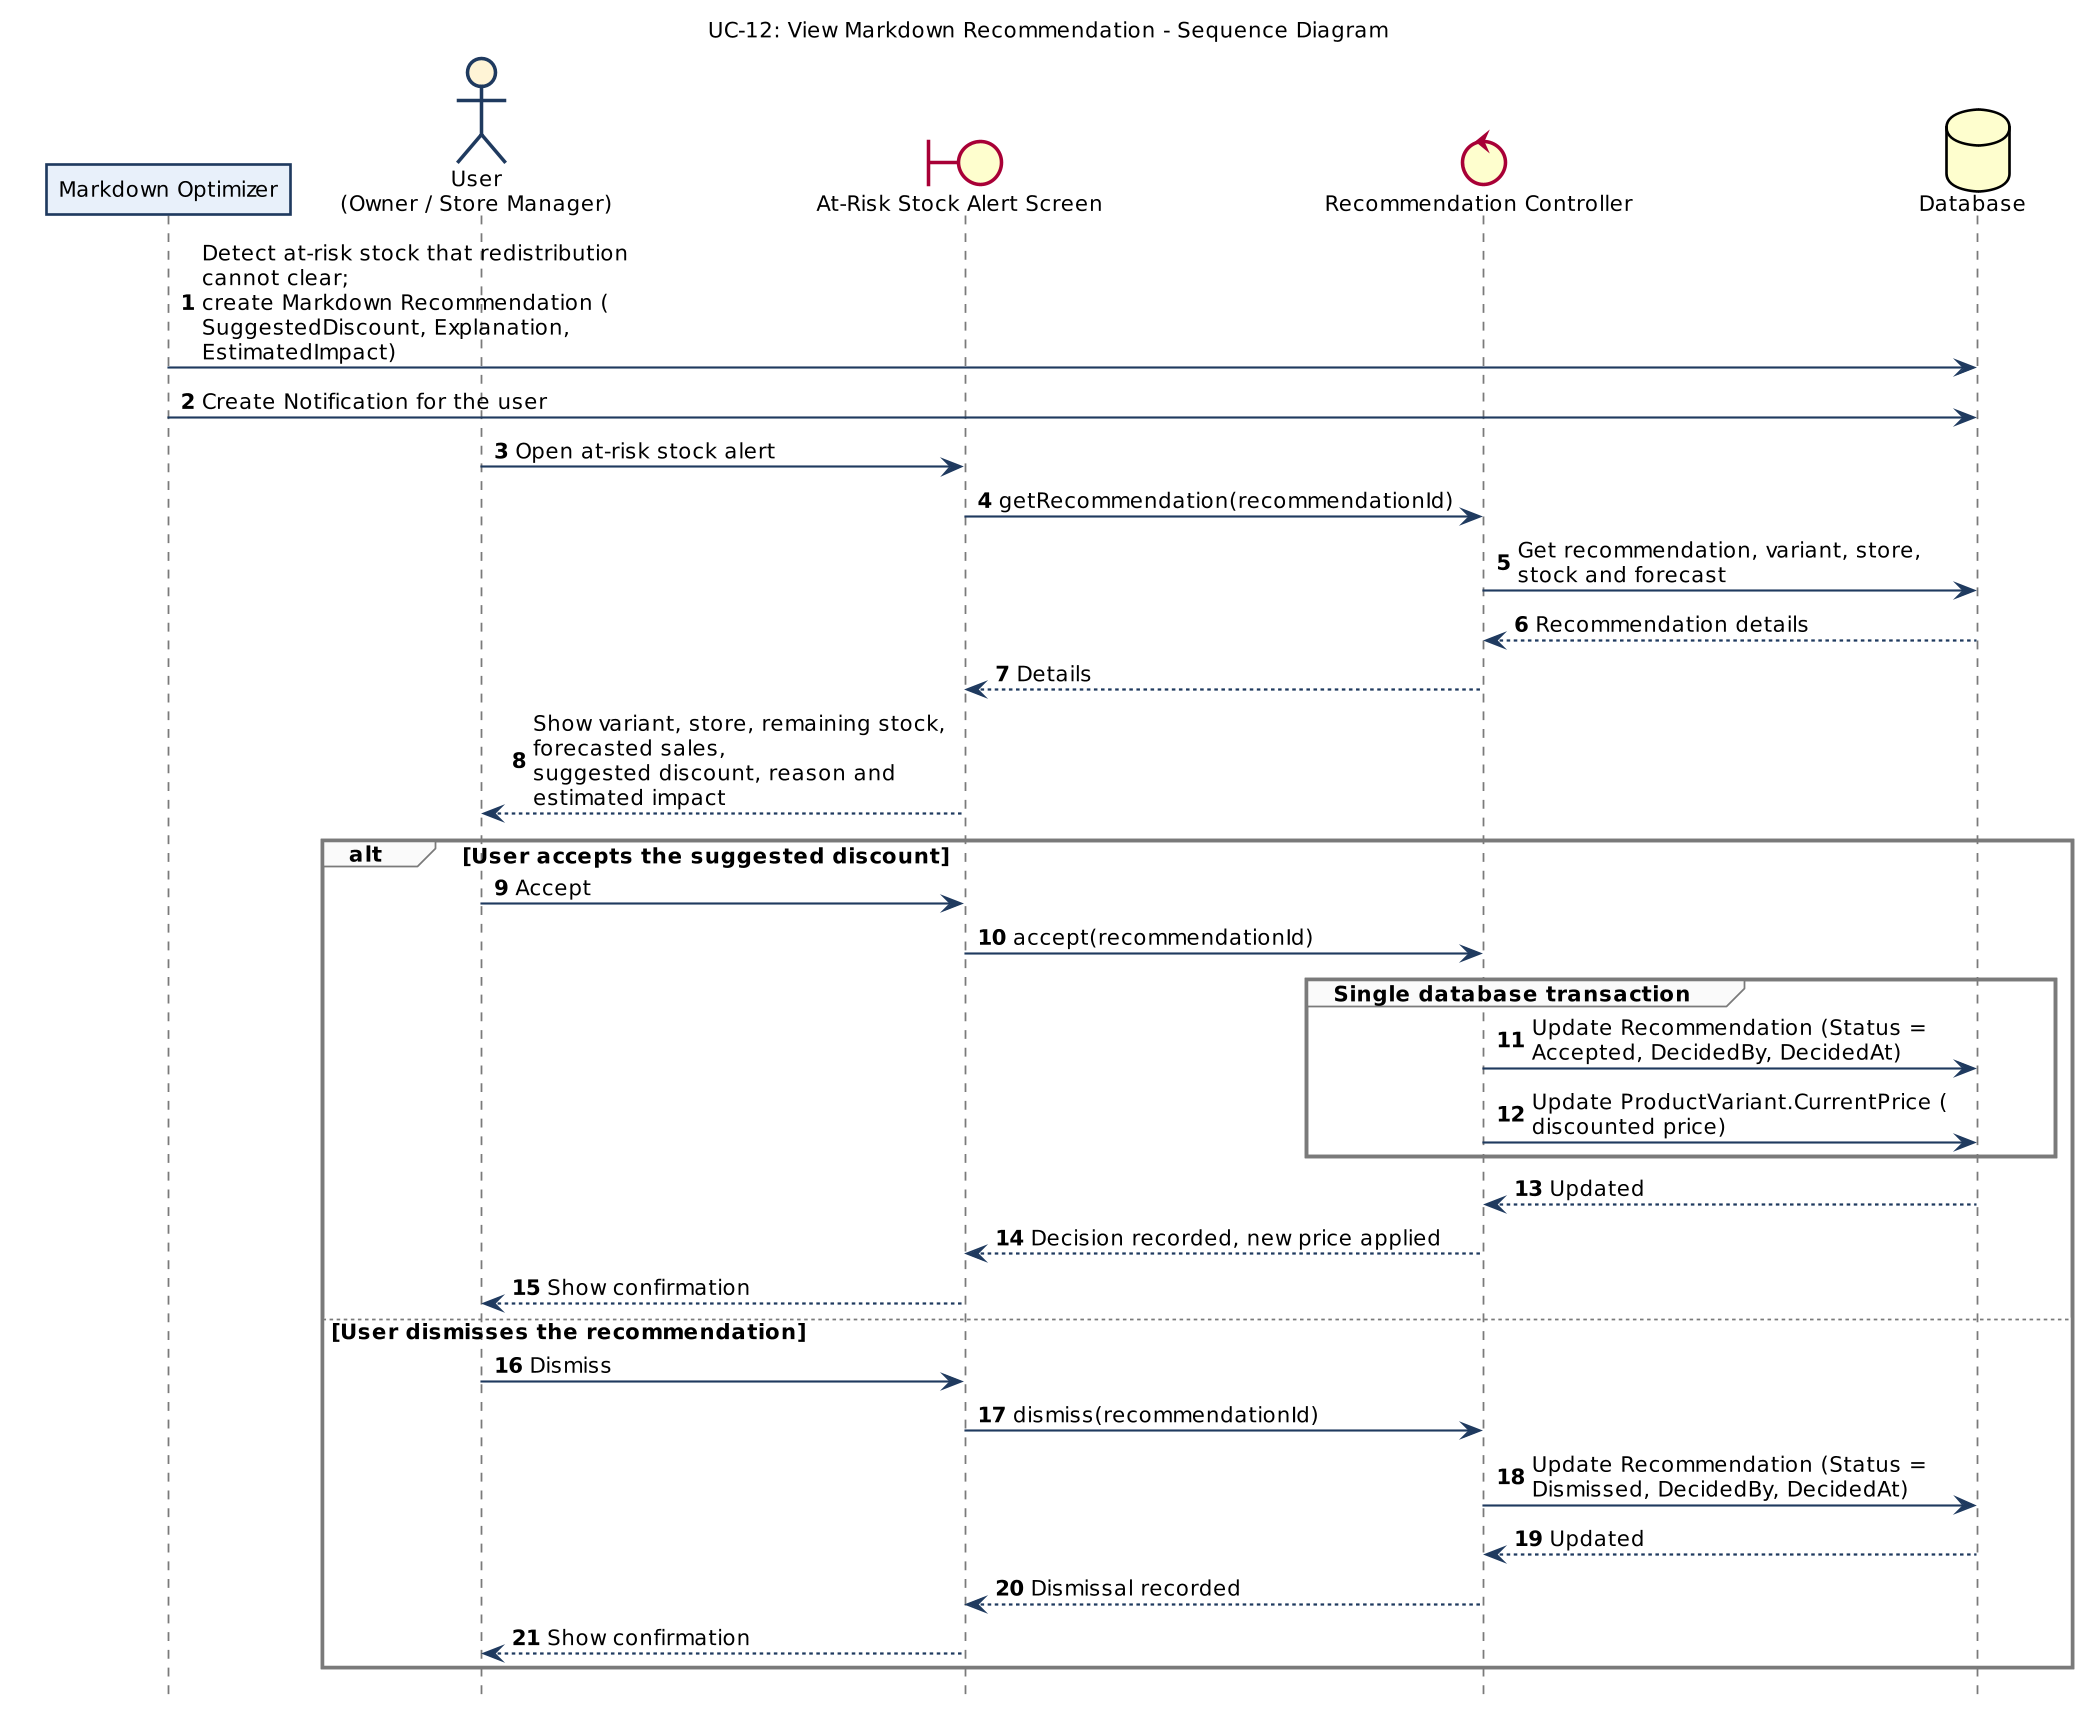
\includegraphics[width=\textwidth,height=0.85\textheight,keepaspectratio]{Figures/SequenceDiagrams/UC12_View_Markdown_Recommendation.png}
    \caption[Sequence Diagram: View Markdown Recommendation]{Sequence Diagram: View Markdown Recommendation\\ This figure shows the sequence diagram of UC-12 (View Markdown Recommendation)}
    \label{fig:seq-uc12}
\end{figure}
 
\subsection{UC-13: View Reorder Recommendation}
 
This diagram shows the interaction for the use case \textbf{View Reorder Recommendation} (UC-13).
 
\begin{figure}[H]
    \centering
    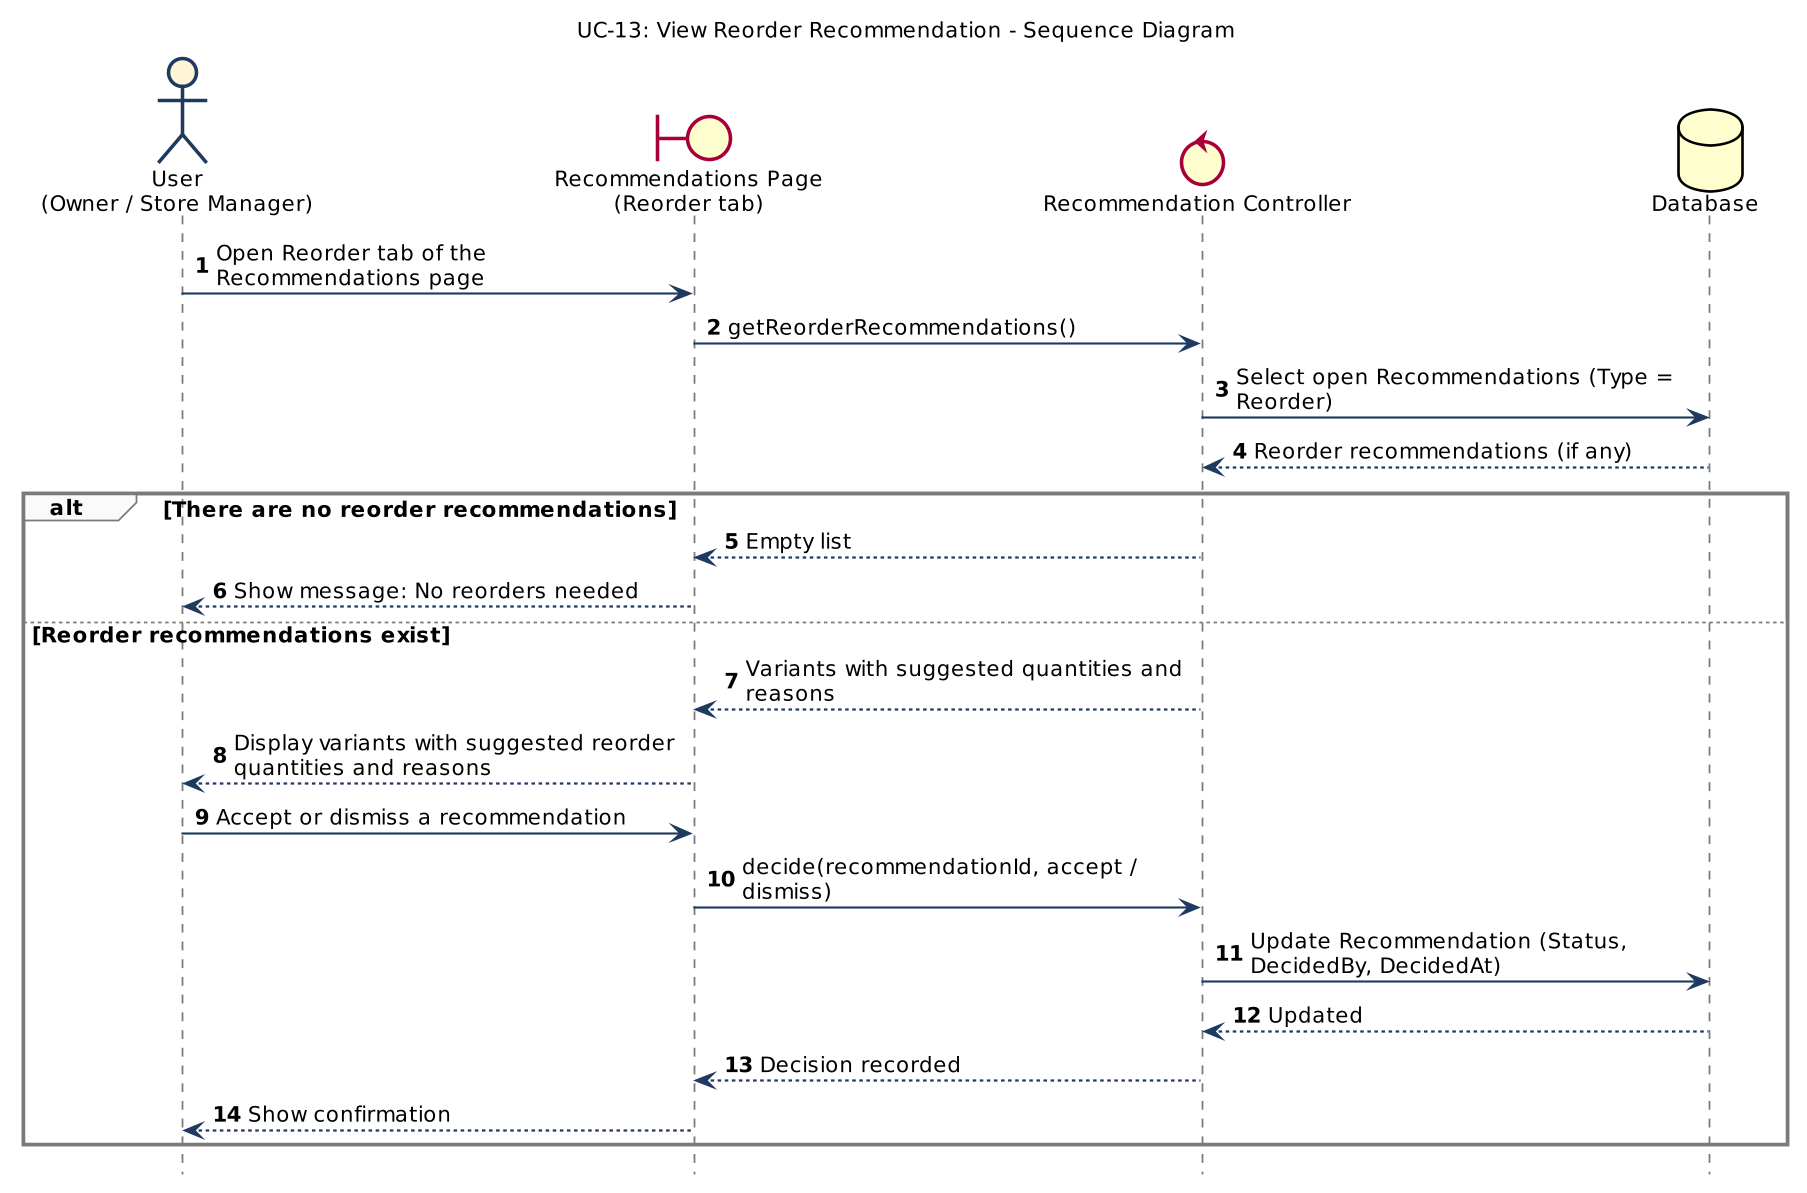
\includegraphics[width=\textwidth,height=0.85\textheight,keepaspectratio]{Figures/SequenceDiagrams/UC13_View_Reorder_Recommendation.png}
    \caption[Sequence Diagram: View Reorder Recommendation]{Sequence Diagram: View Reorder Recommendation\\ This figure shows the sequence diagram of UC-13 (View Reorder Recommendation)}
    \label{fig:seq-uc13}
\end{figure}
 
\subsection{UC-14: Manage Subscription}
 
This diagram shows the interaction for the use case \textbf{Manage Subscription} (UC-14).
 
\begin{figure}[H]
    \centering
    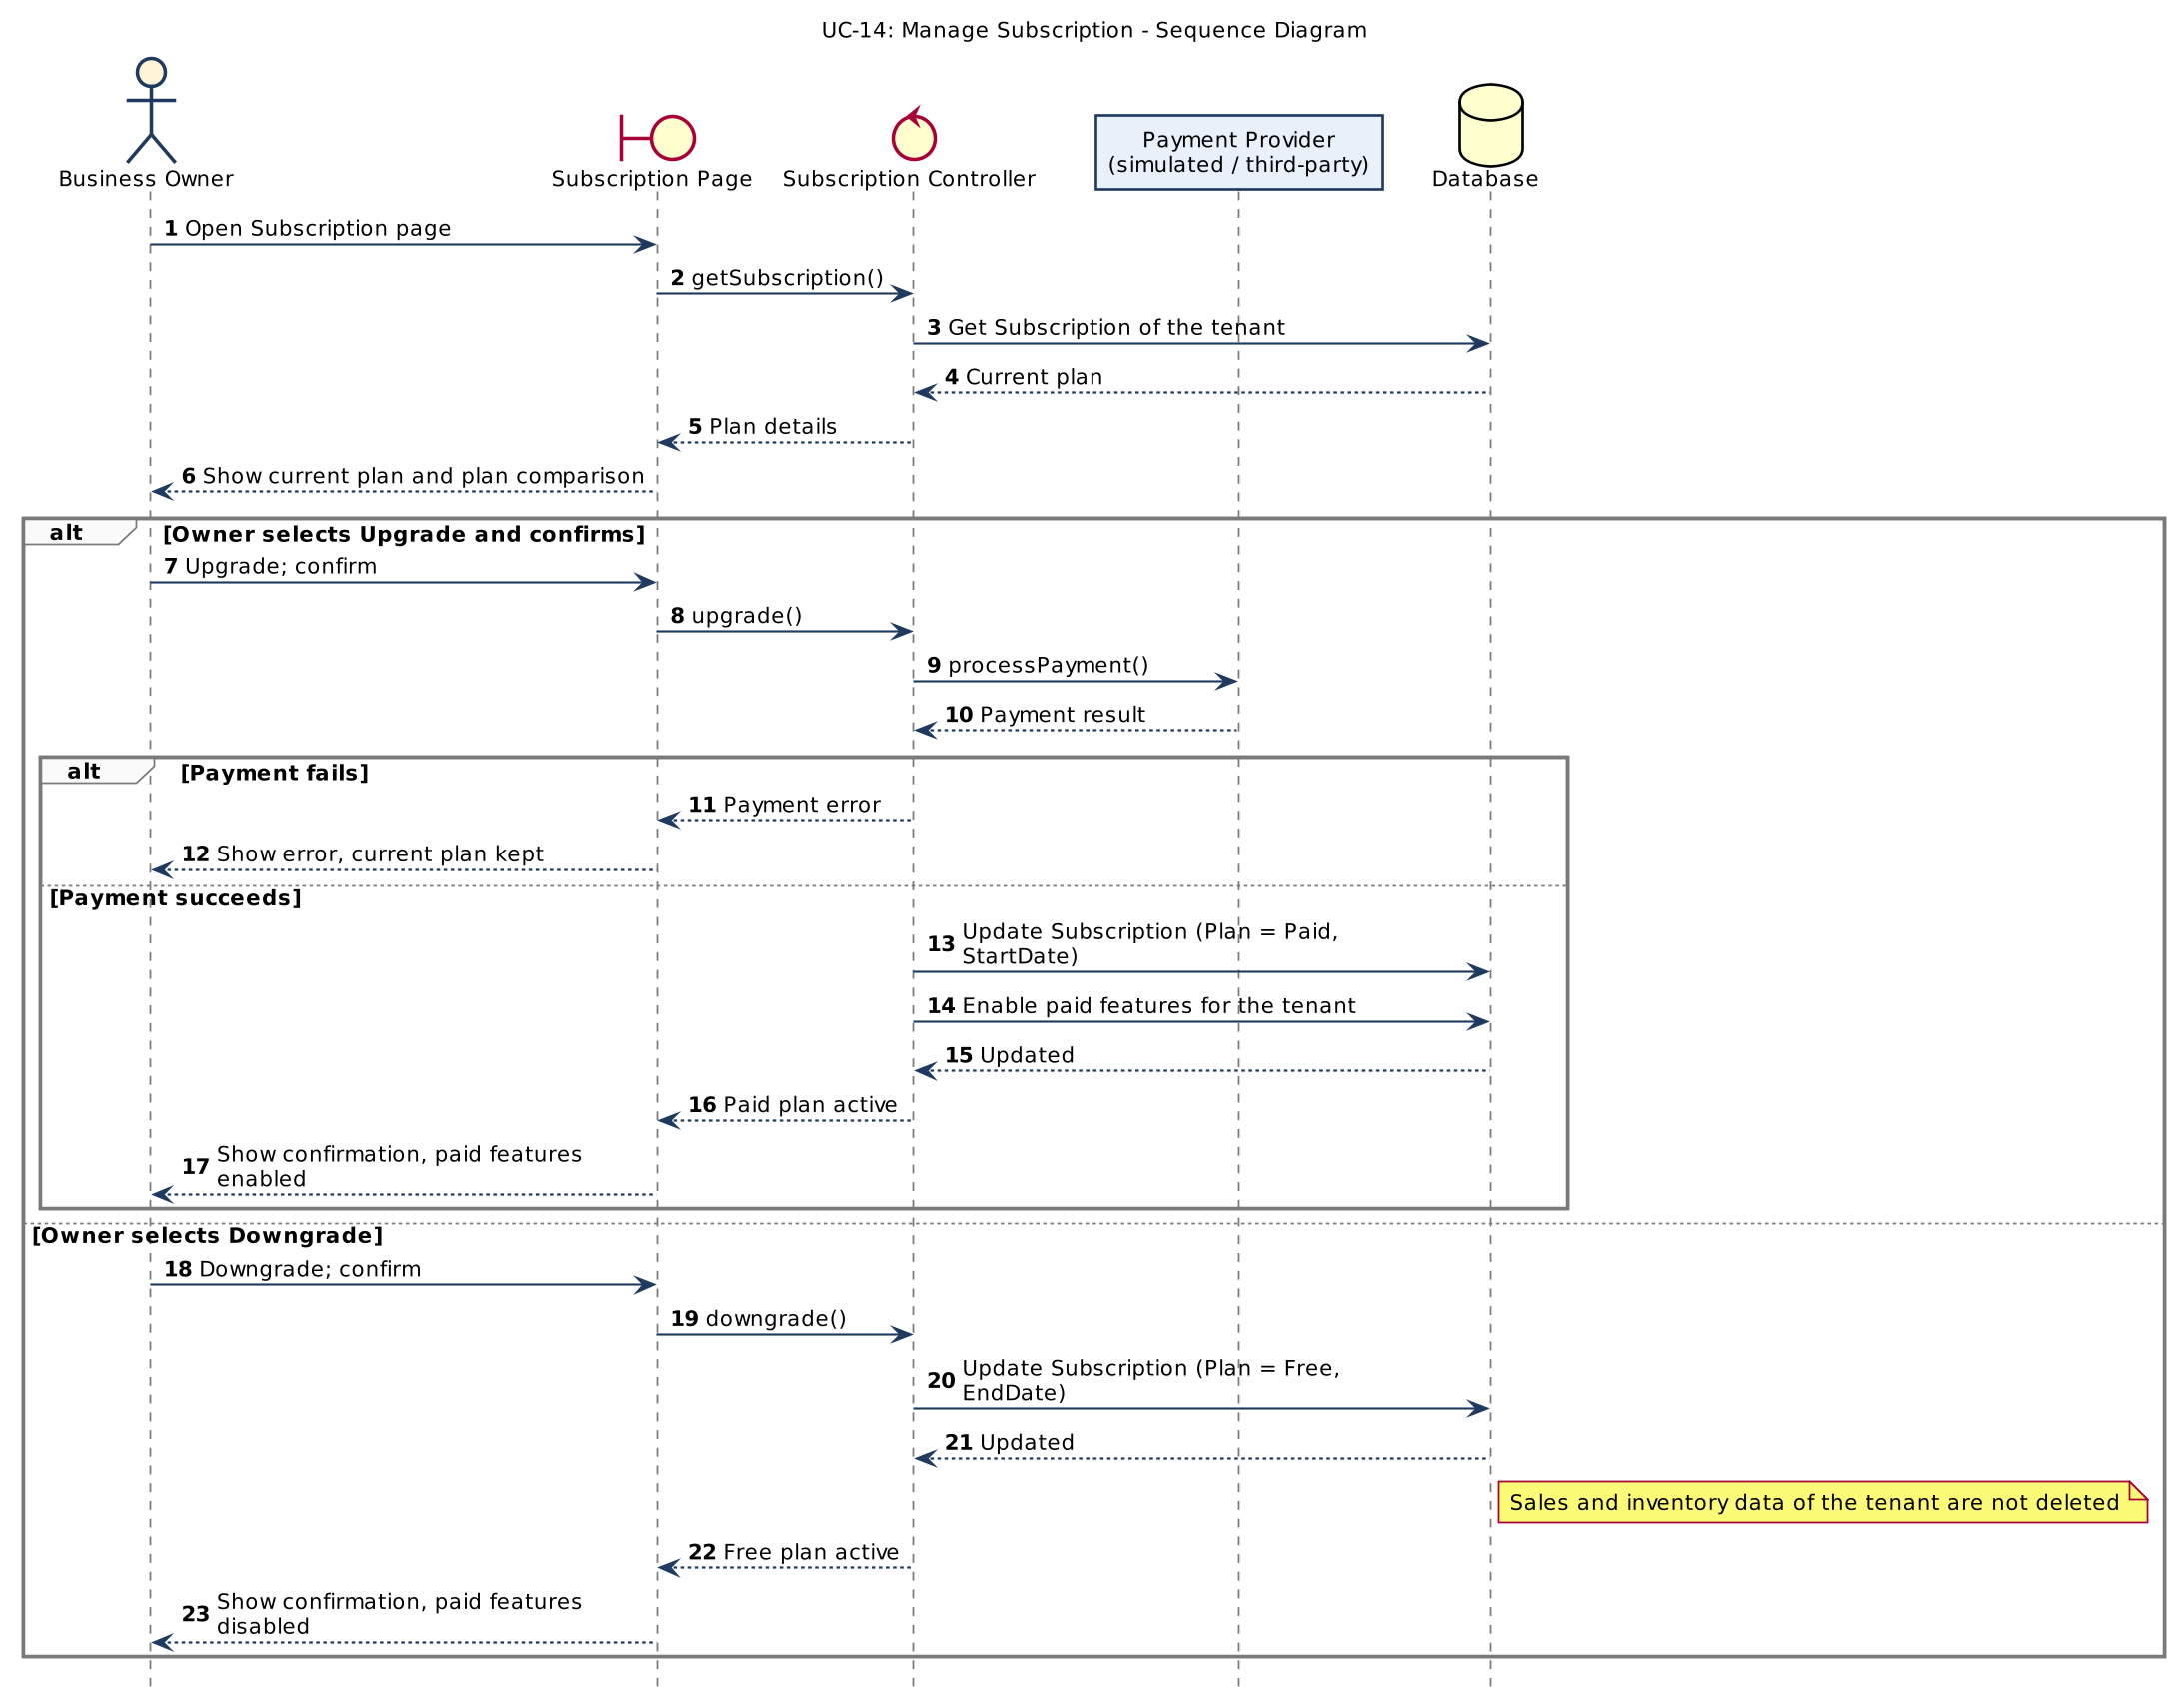
\includegraphics[width=\textwidth,height=0.85\textheight,keepaspectratio]{Figures/SequenceDiagrams/UC14_Manage_Subscription.png}
    \caption[Sequence Diagram: Manage Subscription]{Sequence Diagram: Manage Subscription\\ This figure shows the sequence diagram of UC-14 (Manage Subscription)}
    \label{fig:seq-uc14}
\end{figure}
 
\subsection{UC-15: Manage Tenants}
 
This diagram shows the interaction for the use case \textbf{Manage Tenants} (UC-15).
 
\begin{figure}[H]
    \centering
    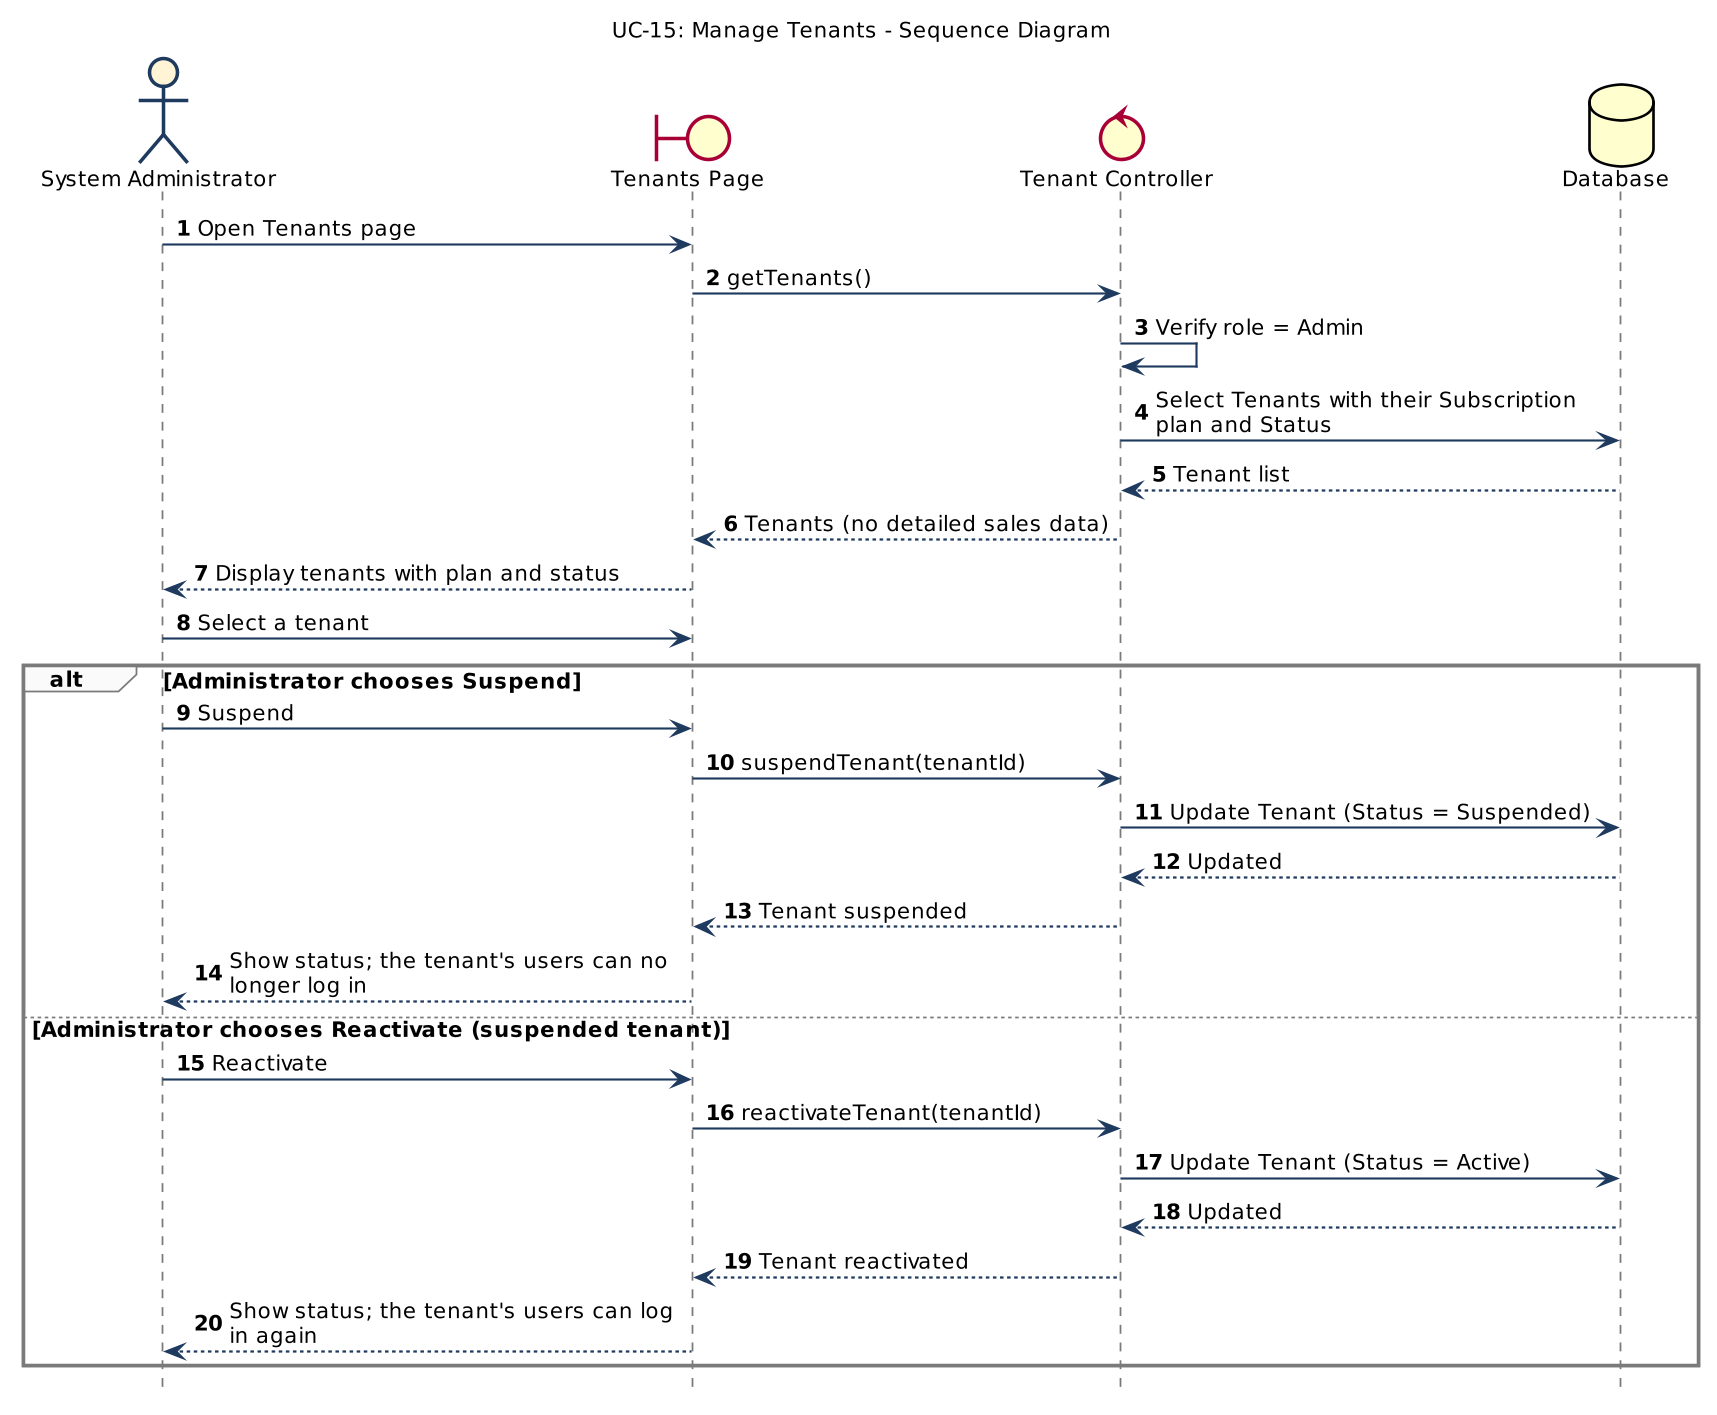
\includegraphics[width=\textwidth,height=0.85\textheight,keepaspectratio]{Figures/SequenceDiagrams/UC15_Manage_Tenants.png}
    \caption[Sequence Diagram: Manage Tenants]{Sequence Diagram: Manage Tenants\\ This figure shows the sequence diagram of UC-15 (Manage Tenants)}
    \label{fig:seq-uc15}
\end{figure}

\section{Policies and Tactics}

While creating StockSense, the following policies and tactics will be applied:

\subsection{Tools to be Used}

A number of tools and libraries will be employed to develop StockSense. The most important ones are:

\begin{itemize}
    \item The web dashboard and the POS screens will be created using React.
    \item The backend REST API will be implemented with Python and FastAPI or Django to handle authentication, tenant checks, and communication between the modules.
    \item All business data will be stored in PostgreSQL, and there will be a tenant identifier on each table that holds data for a business.
    \item The uploaded CSV and Excel files will be read, cleaned, and normalized using pandas and openpyxl.
    \item Data preparation, grouping of similar series, and calculation of error metrics will be supported using scikit-learn and NumPy, with LightGBM as the primary model for demand forecasting and simple statistical baseline models calculated using statsmodels.
    \item Version Control: Git and GitHub will be used to manage the software versions.
    \item Development: Visual Studio Code will be used for development.
    \item API testing: Postman will be used for API testing.
    \item Model experiments: Jupyter Notebook will be used for model experiments.
\end{itemize}

\subsection{Coding Guidelines and Conventions}

The backend will be written in Python, and the forecasting code in the same language, while the frontend will be implemented using a combination of JavaScript and React. The team will use a naming convention and write functions to be brief and easy to read, adding comments when the logic is not clear. The code will be kept organized by having each module reside in its own package. All changes will be checked by another team member before they are merged. Safe coding techniques will be observed throughout, such as storing passwords only in hashed form, parameterising database queries, and never storing secret keys in the repository.

\subsection{User Interface}

StockSense is designed for non-technical stock owners and managers and should be simple and easy to use, with minimal training required and clear navigation. A new user should be able to make a first sale without having to read any documentation. Forecasts will be presented as charts next to previous sales, and each recommendation is accompanied by a short explanation in plain language. Simple words will also be used to write error messages, e.g., if an uploaded file contains an error, this will be explained in a plain-language error message. The interface will be available on desktop computers, tablets, and phones.

\subsection{Extensibility}

The system will be designed in terms of modules, with each module having a specific function: POS and inventory, data ingestion, forecasting, recommendations, and markdown optimization. These modules will communicate through clear interfaces, which means that if one module is changed, the others do not need to change. The forecasting module will have a structure that allows various models to be tested and replaced without re-designing the application. The forecasting engine is general purpose and can be used by any business that stocks products with variants, sizes, or multiple stores, with new recommendation rules added as needed.

\subsection{Tenant Data Isolation and Security}

Each record in the system will be assigned to a tenant, and the backend will verify tenant ownership before each request reads or updates any data. Features will be accessible based on the role of the user, such that a store manager will only be able to view and update data of the store they have been assigned to. All communication will be via HTTPS. The system administrator can set up tenants and plans but will not be able to view the granular sales data unless required as part of support.

\subsection{Data Validation}

Uploaded sales files will be verified prior to being submitted to the forecasting pipeline. Invalid and incomplete rows will be flagged or rejected, and an upload report will inform the owner of what was accepted and what was rejected. In case an upload fails halfway, the data already stored will not be affected.

\subsection{Explainable Recommendations}

If a recommendation is made, the primary reasons for the recommendation (forecast, current stock, surplus/shortage, source branch) will be saved with it, including a financial impact estimate. This enables the owner to see the reason for each suggestion on the dashboard rather than just a number.

\subsection{System Testing}

StockSense will have a testing policy that will involve unit testing, integration testing, and end-to-end testing. Individual tests will be executed on the parts of the system, including the validation rules and the inventory update after a POS sale. The API, database, and modules will be tested for correct integration, and the REST endpoints will also be tested using Postman. End-to-end tests will be completed following full user flows, such as registering a business, logging a sale, uploading a file, and taking action on a recommendation. Some tests will be specific to this project: tenant separation will be checked for data leakage, role-based access will be tested with each user type, and the upload pipeline will be tested with incomplete and poorly formed files. The forecasting models and the statistical baseline will be compared using MAPE and RMSE on a data set that the models have not seen before. The performance requirements from the requirements chapter (e.g., saving a POS sale within 2 seconds, processing a file of 100,000 rows within 5 minutes) will also be tested prior to release.

\subsection{Software Maintenance}

The code will be maintained in a version-controlled repository on GitHub, and bugs and tasks will be tracked so that issues are not lost. Failed uploads, rejected records, and failed forecasting runs will be logged, making it easier to identify the cause. The models will be updated frequently with fresh data, as forecast accuracy diminishes when sales patterns change. The database will be backed up regularly to allow recovery of business data in the event of a failure. New team members will be able to grasp the system rapidly through up-to-date code and design documents.

\subsection{Algorithms}

The algorithms used in StockSense will be selected considering time efficiency and space efficiency, and will be verified by Big-O analysis to ensure that they scale with the number of tenants and the size of the sales history. Gradient-boosted trees (LightGBM), a method suitable for large retail data that performed very well in the M5 competition, will be used to forecast demand. One common model will be trained for each tenant across its products, sizes, and stores. A new tenant must first record or upload enough sales history, and until then no forecast is shown. Simple statistical models from statsmodels will be retained as a baseline to show whether the more complicated model is truly necessary. The recommendation algorithm will compare the forecast demand to the current stock of all branches for each variant. It will match branches with surplus to branches where a shortage is expected, then scan the remaining slow-moving stock to propose a markdown, and lastly suggest a reorder. The markdown logic will raise an alert when an item's selling speed indicates that the stock will not clear in time, so that corrective measures can be taken early. Most businesses do not have many branches, so this matching remains low cost. Large uploads and model training will be performed in the background to keep the system fast, the most recent forecasts will be saved rather than re-calculated when served, and the database will be indexed on the tenant identifier and the main keys.

\section{Conclusion}

In this chapter, the high level as well as the low level design of StockSense was explained. The proposed architecture separates out the tenant management, POS/inventory operations, data ingestion, forecasting, recommendations, and reporting on the dashboard into distinct modules. Tenant isolation, role-based access, data validation, background processing, and database indexing provide the foundation for a secure and scalable system. The design also supports the project's main decision flow: forecast demand, redistribute existing stock where possible, recommend markdowns for remaining slow-moving stock, and reorder only when necessary. The testing and maintenance strategy will be used to ensure the system is correct, performs well, is secure, and will be accurate before it is put into use.
\bibliographystyle{IEEEtran}
\bibliography{fypbib}

\end{document}